% PhD thesis template, Lund University
% Originally designed for the Faculty of Science: Astronomy and
% Theoretical Physics
% Modified for the Faculty of Medicine: Clinical Sciences
%
% This version by: Christian Brueffer (2017-2020)
% Prev versions by: Daniel Carrera (September 2016),
%                   Daniel Michalik (2015-1016?)
% Other editors:   Berry Holl, Helene Jönsson, Jonas Palm
%
% Original editor: Berry Holl
% 
% Instructions: Use "xelatex". This is required to support the fonts
% used by Lund University. The fonts need to be installed first, see
% README.txt for instructions.
%
% If you use (pdf)latex instead, the default latex fonts will be used. 
% That would be a pity, cause the Garamond/Frutiger suggestion by the
% University looks much nicer for your thesis!
%
\documentclass[11pt]{book} 

% ==================================
% PACKAGES
% ==================================

% Make \cleardoublepage insert an empty page without a page number.
\usepackage{emptypage} 
\usepackage{blindtext}	% For "Lorem Ipsum" style place holders
\usepackage{graphicx}	% For \includegraphics
\usepackage{amsfonts}	% Math symbols
\usepackage{amsmath}	% Math symbols
\usepackage{amssymb}	% Math symbols
\usepackage{pdfpages}	% To include the PDFs of the papers
\usepackage{moresize}	% Additional font sizes \HUGE and \ssmal.
%\usepackage{pageslts}  % To calculate the total number of pages
\usepackage{enumerate}  % more enumeration options, e.g. roman numerals
\usepackage{enumitem}   % more itemize flexibility
\usepackage{parskip}    % paragraph spacing
\usepackage{longtable}  % needed by tabu
\usepackage{tabu}       % long table
\usepackage{rotating}   % for sidewaysfigure
\usepackage{textcomp}   % for \textcopyright
\usepackage[super]{nth} % for nice formatting of "2nd" etc


% ------------------------------------------------- %
% Hyperlinks
%
\definecolor{myblue}{RGB}{0, 114, 178}
\definecolor{myyellow}{RGB}{230, 159, 0}
\usepackage[colorlinks=false,
            linkbordercolor=myblue,
            citebordercolor=myblue,
            urlbordercolor=myyellow,
            %hidelinks,
            % PDF metadata
            pdftitle={RNA Sequencing for Molecular Diagnostics in Breast Cancer}
            pdfauthor={Christian Brueffer},
            pdfsubject={RNA Sequencing for Molecular Diagnostics in Breast Cancer},
            pdfkeywords={Breast cancer, RNA sequencing, diagnostics, biomarkers, mutations},
            ]{hyperref}


% Hyphenation, support for different languages, last one is default
% Make sure to install the hyphenation packages for all languages you need
\usepackage[ngerman,british]{babel} 

% ==================================
% PAGE SIZE -- G5 OR E5
% ==================================

% G5 format (larger)
\usepackage[paperwidth=169mm,paperheight=239mm,total={13.3cm,19.6cm}, top=1.8cm, ignorehead, centering, footskip=\footskip+4mm ]{geometry}

% E5 format (smaller)
%\usepackage[paperwidth=155mm,paperheight=220mm,total={12cm,18cm}, top=1.8cm, ignorehead, centering, footskip=\footskip+4mm ]{geometry}


% ==================================
% CONFIGURE THE FONTS
% ==================================
\usepackage{ifxetex}
\usepackage{mathspec}
\usepackage[no-math]{fontspec}
\usepackage{xunicode}
\usepackage{xltxtra}
\AtBeginEnvironment{tabular}{\addfontfeatures{Numbers={Monospaced}}}
\AtBeginEnvironment{tabularx}{\addfontfeatures{Numbers={Monospaced}}}

%
% (1) If the font is installed in your system:
%
%\setmainfont{Adobe Garamond Pro}
%\setsansfont{Frutiger LT Std 45 Light}
%\setmathfont(Greek,Digits,Latin){Adobe Garamond Pro}

%
% (2) If the fonts in the local directory.
%
\setmainfont[
  Ligatures=TeX,
  Extension=.otf,
  UprightFont=*-Regular,
  BoldFont=*-Semibold,
  ItalicFont=*-Italic,
  BoldItalicFont=*-Italic,
]{AGaramondPro}
\setsansfont{[FrutigerLTStd-Light.otf]}
%\setmathfont(Greek,Digits,Latin){[AGaramondPro-Italic.otf]}

% mathspec is broken. The next eight lines work around that.
\usepackage{etoolbox}
\makeatletter
\begingroup\lccode`~=`"
\lowercase{\endgroup
  \everymath{\let~\eu@active@quote}
  \everydisplay{\let~\eu@active@quote}
}
\makeatother


% ==================================
% CHAPTERS, SECTIONS, SUBSECTIONS WITHOUT NUMBERS
% ==================================
% define commands for chapters, sections, and subsections
% that do not have a number, but are entered as candidates
% for the table of contents.
\newcommand\chap[1]{%
  \chapter*{#1}%
  \addcontentsline{toc}{chapter}{#1}
  \markboth{#1}{#1}
}
\newcommand\sect[1]{%
  \section*{#1}%
  \addcontentsline{toc}{section}{#1}
  \markright{#1}
}
\newcommand\subsect[1]{%
  \subsection*{#1}%
  \addcontentsline{toc}{subsection}{#1}
}


% ------------------------------------------------- %
% ------------------------------------------------- %
% ------------------------------------------------- %
% ------------------------------------------------- %

% Must come in the beginning. Changes the spacing in the table of contents to look more pleasing
\usepackage{tocloft}
\setlength{\cftbeforepartskip}{5.0mm}
\setlength{\cftbeforechapskip}{2.0mm}
\setlength{\cftbeforesecskip}{0.0mm}

% figure captions in bold (i.e. "Figure 1" in bold), sans serif, smaller font size, hanging label, always starting on the left side
\usepackage[
  font=small,
  labelfont=bf,
  labelsep=period
]{caption}

% figures centered, smaller font in tables, captions on top for tables
% caption/table footnotes small
\usepackage[]{floatrow}
\DeclareFloatFont{tiny}{\tiny} % "scriptsize" is defined by floatrow, "tiny" is not
\DeclareFloatFont{ssmall}{\ssmall}
\floatsetup[table]{font={footnotesize},position=top}
\captionsetup{footfont=footnotesize}
%%%%%%%%%%%%%%%%%%%%%%%%%%%%%%%%%%%% end fonts %%%%%%%%%%%%%%%%%%%%%%%%%%%%%%%%%%%%%%%%%%%%%%%%%%%%%%%

% Table formatting
\usepackage{tabularx}  % For tables spanning the full text width
\usepackage{booktabs}  % Commands to improve tabular; including horizontal rulers
\usepackage{multirow}

% Chapters should have numbers - a typical thesis consists of two chapters:
% One to introduce and summarize the research ("kappa"), and one for
% reproductions of the papers and manuscripts. No need to number them by default.
% If you need chapter numbers back, comment the following line.
%\renewcommand{\thesection}{\arabic{section}} 

% Sections and subsections have numbers, subsubsections etc do not.
\setcounter{secnumdepth}{2}

% Only chapters and sections appear in the table of contents, not subsections etc
\addtocontents{toc}{\protect\setcounter{tocdepth}{1}}  % sections
%\addtocontents{toc}{\protect\setcounter{tocdepth}{2}}  % subsections
%\addtocontents{toc}{\protect\setcounter{tocdepth}{3}}  % subsubsections

% not every page needs to go to the same bottom line. Allows nicer page breaks.
%\raggedbottom

% avoid orphan/widow lines. Lower this number if necessary to get a good layout.
\widowpenalty500
\clubpenalty500
\interfootnotelinepenalty=10000  % prevent footnote splitting across two pages

% paragraph settings
\setlength{\parskip}{2mm}

% Small caps serif font, for Paper numbers, ISBN, etc
\newcommand{\I}{\textrm{\scshape i}\xspace}
\newcommand{\II}{\textrm{\scshape ii}\xspace}
\newcommand{\III}{\textrm{\scshape iii}\xspace}
\newcommand{\IV}{\textrm{\scshape iv}\xspace}
\newcommand{\V}{\textrm{\scshape v}\xspace}
\newcommand{\VI}{\textrm{\scshape vi}\xspace}
\newcommand{\VII}{\textrm{\scshape vii}\xspace}
\newcommand{\VIII}{\textrm{\scshape viii}\xspace}
\newcommand{\IX}{\textrm{\scshape ix}\xspace}
\newcommand{\X}{\textrm{\scshape x}\xspace}
\newcommand{\ISBN}{\textrm{\scshape isbn}\xspace}
\newcommand{\ISSN}{\textrm{\scshape issn}\xspace}

% Black box for the paper indicators
\usepackage{tikz}
\usetikzlibrary{calc}
\usetikzlibrary{shapes}

\makeatletter
\newdimen\@myBoxSize%
\newcommand{\PaperBox}[2][]{%
    \pgfmathsetlength{\@myBoxSize}{14mm}%
    \tikz \node [shape=rectangle,shape aspect=1,draw=black,fill=black,text depth=.25ex,minimum size=\@myBoxSize,#1] {#2};%
}%
\makeatother

% Footnote without mark in the text
% Source: https://tex.stackexchange.com/questions/30720/footnote-without-a-marker
\newcommand\blfootnote[1]{%
  \begingroup
  \renewcommand\thefootnote{}\footnote{#1}%
  \addtocounter{footnote}{-1}%
  \endgroup
}

%----------------------------------------------------------------------

% Modify how chapter beginnings look
\usepackage{titlesec}

% from https://texblog.org/2012/07/03/fancy-latex-chapter-styles/
\definecolor{gray75}{gray}{0.75}
\newcommand{\hsp}{\hspace{20pt}}
\titleformat{\chapter}[hang]{\Huge\bfseries}{\thechapter\hsp\textcolor{gray75}{|}\hsp}{0pt}{\Huge\bfseries}
% left / before / after
\titlespacing*{\chapter}{0pt}{-20pt}{0pt}

% Spacing between sections, subsections, and subsubsections
\titlespacing*{\section}{0pt}{2em}{1.2em}
\titlespacing*{\subsection}{0pt}{1.5em}{0.8em}
\titlespacing*{\subsubsection}{0pt}{1.5em}{0.7em}

%----------------------------------------------------------------------

% Quotes at the beginning of chapters
\usepackage{epigraph}
\setlength\epigraphwidth{0.5\textwidth}
\setlength\epigraphrule{0pt}  % no line between
\renewcommand*{\epigraphsize}{\normalsize\itshape}


%%%%%%%%%%%%%%%%%%%%%%%%%%%%%%%%%%%%%%%%%%%%%%%%%%%%%%%%%%%%%%%%%%%%
% Define nice headers and footers
% To keep the thesis non-cluttered we only put the page number into
% the footer, and avoid headers
\usepackage{fancyhdr}
\fancyheadoffset{0cm}
\pagestyle{plain}
%page number in the foot centre 
\cfoot{\fancyplain{\thepage}{}}


%%%%%%%%%%%%%%%%%%%%%%%%%%%%%%%%%%%%%%%%%%%%%%%%%%%%%%%%%%%%%%%%%%%%
% Biblatex
%
% Manual: http://ctan.imsc.res.in/macros/latex/contrib/biblatex/doc/biblatex.pdf
% Modification quick guide: https://tex.stackexchange.com/questions/12806/guidelines-for-customizing-biblatex-styles
\usepackage{csquotes}
\usepackage[
backend=biber,
style=nature,
sorting=none,
%sorting=nty,
giveninits=true,  % abbreviate first names
doi=false, 
eprint=false, 
url=false,
isbn=false,
minnames=3,
maxnames=3,
hyperref=true,
backref=true
]{biblatex}
\setlength\bibitemsep{0.5\baselineskip}
\addbibresource{Mendeley.bib}
\addbibresource{miscrefs.bib}

% Customize back references.
\DefineBibliographyStrings{english}{%
  backrefpage = {cited on page},    % originally "cit. on p."
  backrefpages = {cited on pages},  % originally "cit. on pp"
}

% Prevent bibliography entries spanning pages and similar issues.
% Source: https://tex.stackexchange.com/questions/305759/prevent-page-and-column-breaks-mid-bibliography-entries-in-biblatex-biber
\patchcmd{\thebibliography}{\clubpenalty4000}{\clubpenalty10000}{}{}      % no orphans
\patchcmd{\thebibliography}{\widowpenalty4000}{\widowpenalty10000}{}{}    % no widows
\patchcmd{\bibsetup}{\interlinepenalty=5000}{\interlinepenalty=10000}{}{} % no break of entry


% ==================================
% REUSABLE
% ==================================

% Needs matching changes in preamble.tex for PDF metadata!
\newcommand{\myName}{Christian Brüffer}
\newcommand{\myMainTitle}{RNA Sequencing for Molecular Diagnostics in Breast Cancer}
\newcommand{\mySubTitle}{}

\title{Thesis: \myMainTitle}

% Prevent hyphenation
\newcommand{\scanb}{\mbox{SCAN-B}}

% ==================================
% USED IN THE COVER PAGE
% ==================================
\newcommand{\myDegree}{DOCTORAL DISSERTATION}
\newcommand{\myAdvisors}{Dr.~Lao~H.~Saal, Prof.~Håkan~Axelson, Prof.~Mattias~Höglund}
\newcommand{\myOpponent}{Dr.~Aleix~Prat,~MD~PhD}
\newcommand{\myOpponentAffiliation}{\vspace{3mm} Hospital Clínic de Barcelona \\ \vspace{1mm} Institut d'Investigacions Biomèdiques August Pi i Sunyer (IDIBAPS) \\ \vspace{1mm} University of Barcelona \\ \vspace{2mm} Barcelona, Spain}


% ==================================
% DEFENCE ANNOUNCEMENT
% ==================================
\newcommand{\myDefenceDate}{Wednesday the \nth{13} of January 2021 at 13:00}
\newcommand{\myLectureHall}{Room E24, Medicon Village Building 404, Lund}
\newcommand{\myFaculty}{Faculty of Medicine}
\newcommand{\myDepartment}{Department of Clinical Sciences, Lund}
\newcommand{\myDefenceAnnouncement}{%
	by due permission of the \myFaculty, Lund University, Sweden.\\[4mm]
    To be defended in \myLectureHall~on~\myDefenceDate.
}

% Chairperson
%
% Ingrid Hedenfalk, LU
%
% Examination committee
%
% Anne-Vibeke Lænkholm, KU, Department of Clinical Medicine
% Per Karlsson, GU, Oncology
% Björn Nilsson, LU, Division of Hematology and Transfusion Medicine
%
% Substitutes
% Ramin Massoumi, LU
% Anna Hagström, LU

% ==================================
% USED IN THE COPYRIGHT PAGE
% ==================================
% Appears at the top of the page.
\newcommand{\myBlurb}{
	\begin{center}
	\textbf{Main Supervisor} \\
	\vspace{1em}
	Assoc. Prof. Lao H. Saal, MD PhD \\
	Division of Oncology \\
	Department of Clinical Sciences, Lund \\
	Lund University \\
	\vspace{2em}
	\textbf{Co-Supervisors} \\
	\vspace{1em}
    Prof. Håkan Axelson, PhD \\
    Division of Translational Cancer Research \\
    Department of Laboratory Medicine \\
    Lund University \\
	\vspace{0.8em}
    Prof. Mattias Höglund, PhD \\
	Division of Oncology \\
    Department of Clinical Sciences, Lund \\
    Lund University \\
	\vspace{2em}
    \end{center}
}

% Give credit for the front or back covers, if any.
% Give credit for the funding source, if any.
\newcommand{\myCoverFront}{Cover illustration \copyright\, \href{https://www.redbubble.com/people/nobeastsofierce}{nobeastsofierce}}
\newcommand{\myCoverBack}{~} % Use "~" for blank.
\newcommand{\myFundingSource}{~} % Use "~" for blank.
\newcommand{\mySourceLocation}{The \LaTeX{} sources and plot scripts for this thesis are publicly available to enable re-use: \\ \LaTeX{} sources:\hspace{3.6pt} \url{https://github.com/cbrueffer/phd_thesis} \\ Plot scripts:\hspace{11.6pt} \url{https://github.com/cbrueffer/phd_thesis_plots} \\ SCAN-B map: \url{https://github.com/cbrueffer/scanb_map}} % Use "~" for blank.

% ISSN 1652-8220
% ISBN 978-91-8021-008-9
\newcommand{\myCopyrightYear}{2020}
\newcommand{\myISBNprint}{978-91-8021-008-9}
\newcommand{\myISBNpdf}{XXX-XX-XXXX-XXX-X}  % Electronic ISBN.
\newcommand{\myISSN}{1652-8220}
\newcommand{\mySeries}{Lund University, Faculty of Medicine Doctoral Dissertation Series 2021:2}


% ==================================
% MAIN DOCUMENT
% ==================================
\begin{document}

\newgeometry{left=0mm, right=0mm, top=0mm, bottom=0mm}
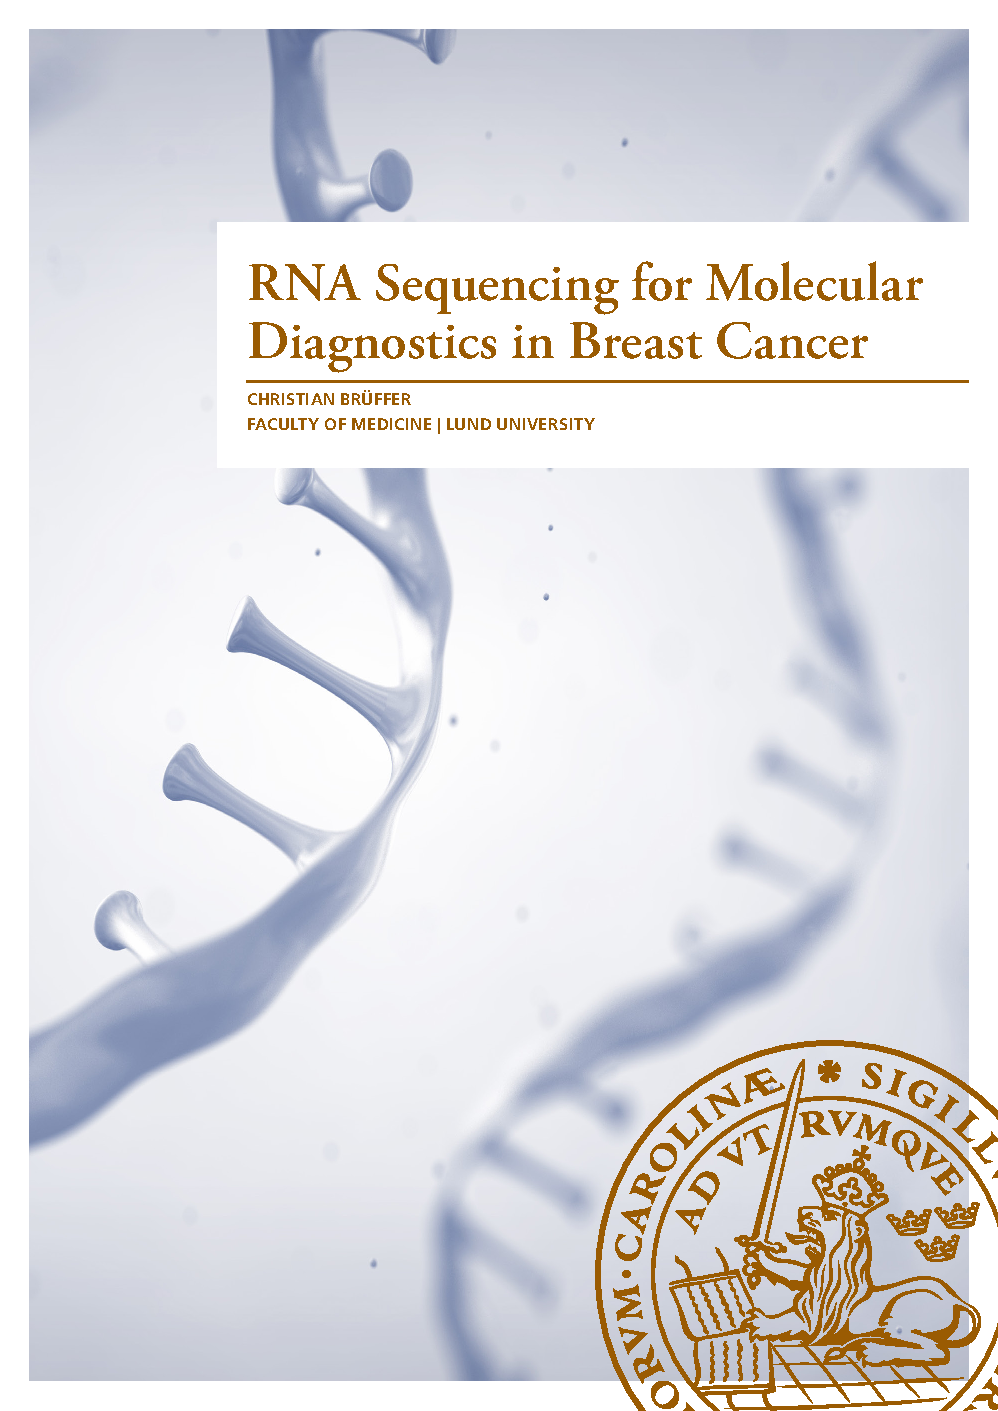
\includepdf[pages=-,width=1.00\textwidth,pagecommand={\thispagestyle{plain}}]{img/front_and_back_cover.pdf}
\restoregeometry

% ==================================
% FRONTMATTER
% ==================================
\frontmatter % roman numbers

% -----------------------------
% Page 1: Title only
% -----------------------------
\thispagestyle{empty} % no page number
\begin{center}
\vspace*{5cm}
{\Huge \myMainTitle}
{\LARGE \mySubTitle}
\end{center}


% -----------------------------
% Page 2: Blank
% -----------------------------
\cleardoublepage
\thispagestyle{empty} % no page number
~

% -----------------------------
% Page 3: Title Page
% -----------------------------
\vfill
\begin{center}
{\Huge \myMainTitle}
\\[2mm]
{\huge \mySubTitle}
\vfill
{\LARGE \myName}

\vfill

\includegraphics[width=0.25\textwidth]{img/LundUniversity_logo.eps}

\vspace{10mm}
{\large \myDegree}\\
\vspace{2mm}
{\large \myDefenceAnnouncement}\\
\vspace{10mm}
{\large\it Faculty opponent}\\
\vspace{5mm}
{\large \myOpponent}\\
{\large \myOpponentAffiliation}
\end{center}
\vfill

% -----------------------------
% Page 4: Insert datasheet
% -----------------------------
%\newpage \thispagestyle{empty} % no page number
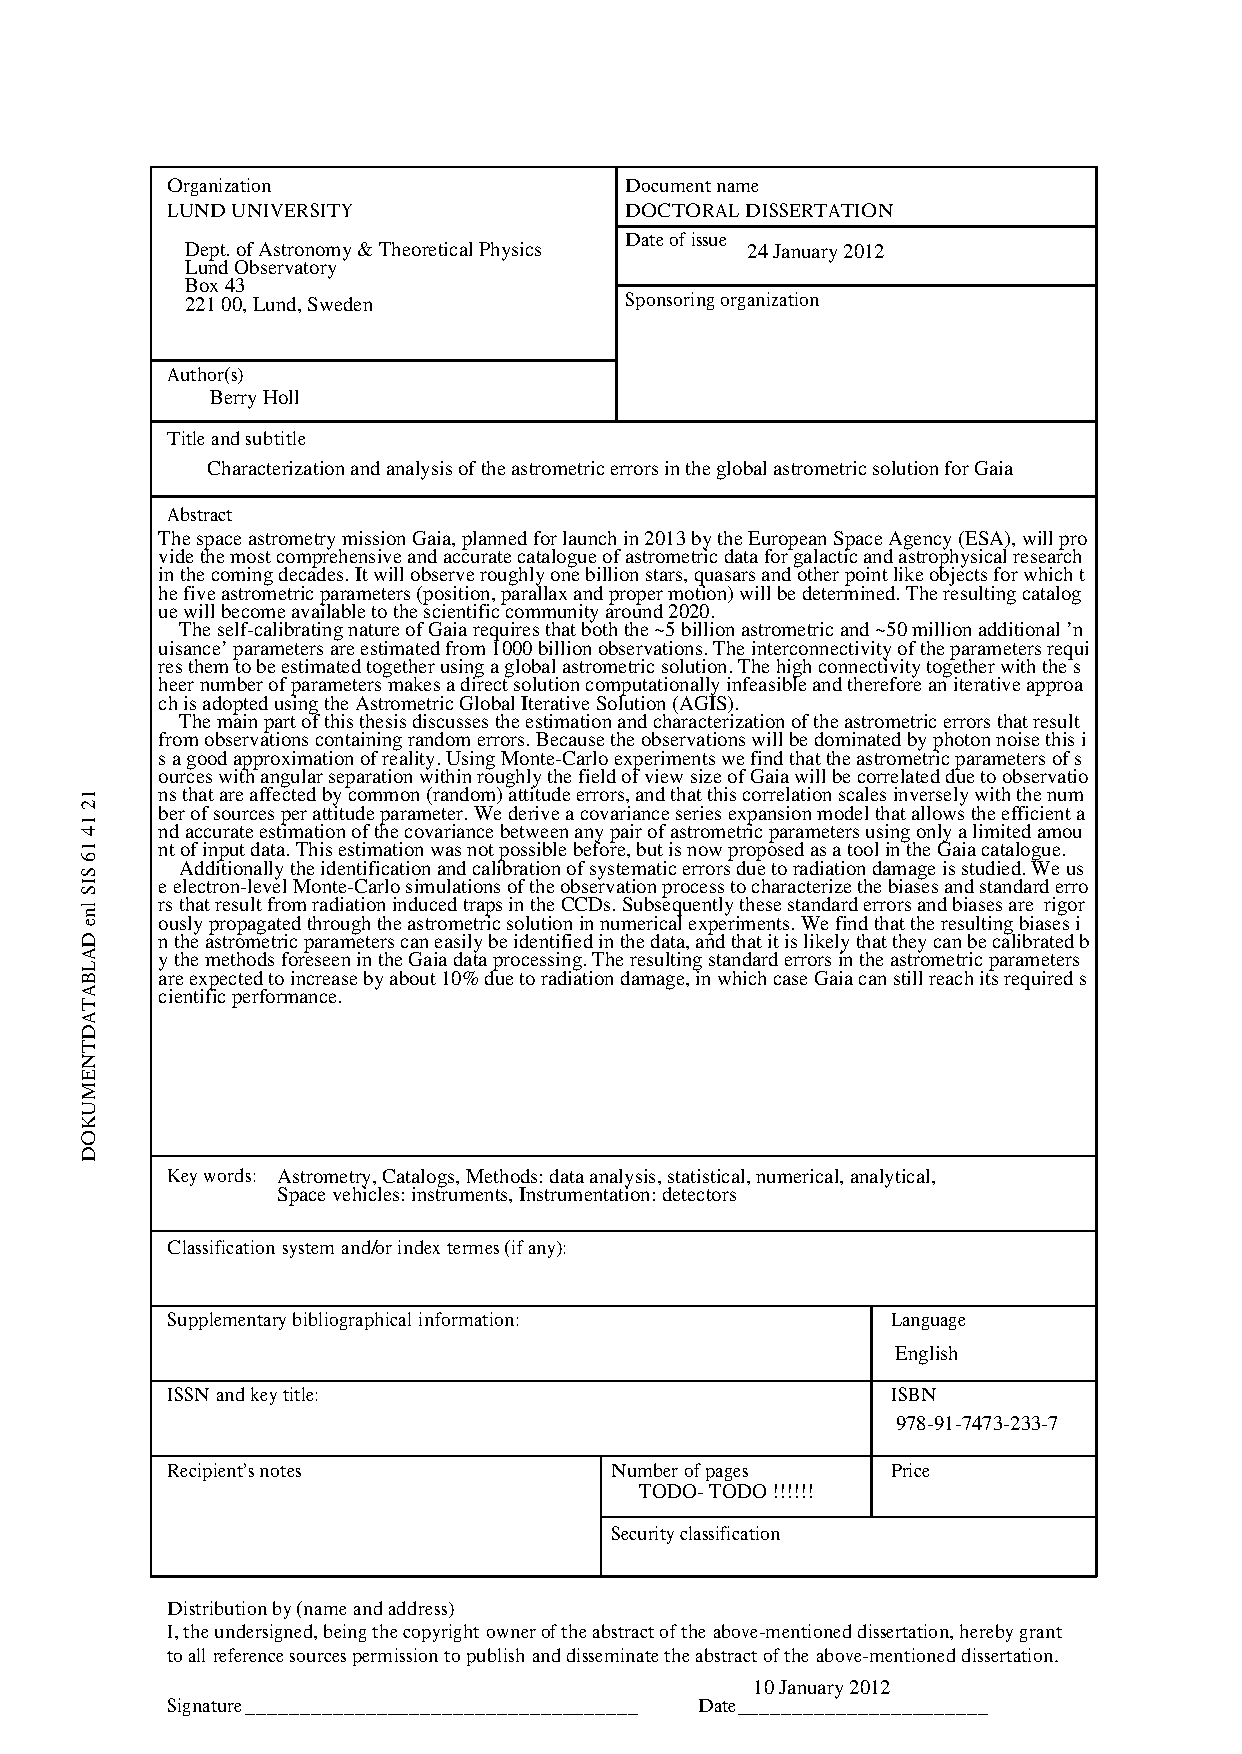
\includepdf{datasheet}

% -----------------------------
% Page 5: Title and author again, with less text.
% -----------------------------
\cleardoublepage
\thispagestyle{empty} % no page number
~
\vfill
\begin{center}
{\Huge \myMainTitle}
\\[2mm]
{\huge \mySubTitle}
\vfill
{\Huge \myName}
\vfill
% black and white (default):

\includegraphics[width=0.25\textwidth]{img/LundUniversity_logo.eps}
\end{center}
\vfill


% -----------------------------
% Page 6: COPYRIGHT INFO
% -----------------------------
\newpage 
\thispagestyle{empty} % no page number
~
\vfill
%\myBlurb
\vfill
{\small
\myCoverFront\\
~
\myCoverBack\\
~
\myFundingSource
\vspace{5mm}
\copyright\, \myName~\myCopyrightYear\\
~
{\myDepartment} \\ \myFaculty, Lund University \vspace{1em} \\
~
\mySourceLocation\\[1em]
~
\mySeries\\
ISBN: \myISBNprint \\ % ISBN av svenska ISBN centralen
%ISBN: \myISBNpdf~(pdf) \\ % ISBN av svenska ISBN centralen
ISSN: \myISSN \\[0.5em]
~
Printed in Sweden by Media-Tryck, Lund~University\\
Lund~\myCopyrightYear\\[4mm]

\includegraphics[width=0.5\textwidth]{img/miljoeloggor}
}



% ==================================
% DEDICATION
% ==================================
\newpage
\thispagestyle{empty} % No page number on quote page
~
\vspace{140pt}
\begin{flushright}
\textit{A tremendous feeling of peace came over him. He knew that at last, for once and for ever,\\it was now all, finally, over.}\\[5pt]--- \textsc{Douglas Adams}, The Hitchhiker's Guide to the Galaxy
\end{flushright}

\cleardoublepage

% ==================================
% TABLE OF CONTENTS
% ==================================
\setcounter{page}{1} % Page Roman 1 of the frontmatter
\tableofcontents
% no page number on toc page:
\addtocontents{toc}{\protect\thispagestyle{empty}}


% ==================================
% LIST OF PUBLICATIONS
% ==================================
\chap{List of Original Studies}

This thesis is based on the following original studies, which are referred to in the text by their Roman numerals:
\vspace{5mm}

% temporarily use footnote symbols to denote equal work on papers
\renewcommand*{\thefootnote}{\fnsymbol{footnote}}

{
\floatsetup[table]{font={normalsize},position=top}
\begin{tabularx}{\textwidth}{rX}

% Paper I
% License: CC-BY 4.0
% https://doi.org/10.1186/s13073-015-0131-9
\I    & \textbf{The Sweden Cancerome Analysis Network-Breast (\scanb{}) Initiative: a large-scale multicenter infrastructure towards implementation of breast cancer genomic analyses in the clinical routine} \vspace{1mm} \\
      & Saal~LH, Vallon-Christersson~J, Häkkinen~J, Hegardt~C, Grabau~D, Winter~C, \textbf{Brueffer~C}, Tang~MHE, Reuterswärd~C, Schulz~R, Karlsson~A, Ehinger~A, Malina~J, Manjer~J, Malmberg~M, Larsson~C, Rydén~L, Loman~N, Borg~Å \vspace{1mm} \\
      & \textit{Genome Medicine, 2015. 7(1):20} \\[5mm]

% Paper II
% License: CC-BY 4.0
% https://doi.org/10.1186/s12859-016-1058-x
% Preprint: https://www.biorxiv.org/content/10.1101/033530v1
\II   & \textbf{TopHat-Recondition: A post-processor for TopHat unmapped reads} \vspace{1mm} \\
      & \textbf{Brueffer~C} and Saal~LH \vspace{1mm} \\
      & \textit{BMC Bioinformatics, 2016. 17(1):199} \\[5mm]

% Paper III
% License: CC-BY 4.0
% https://doi.org/10.1200/PO.17.00135
\III  & \textbf{Clinical Value of RNA Sequencing-Based Classifiers for Prediction of the Five Conventional Breast Cancer Biomarkers: A Report From the Population-Based Multicenter Sweden Cancerome Analysis Network--Breast Initiative} \vspace{1mm} \\
      & \textbf{Brueffer~C}\footnotemark[1], Vallon-Christersson~J\footnotemark[1], Grabau~D, Ehinger~A, Häkkinen~J, Hegardt~C, Malina~J, Chen~Y, Bendahl~PO, Manjer~J, Malmberg~M, Larsson~C, Loman~N, Rydén~L, Borg~Å, Saal~LH \vspace{1mm} \\
      & \textit{JCO Precision Oncology, 2018. 2:1--18} \\[5mm]

% Paper IV
% License: CC-BY-4.0
% https://doi.org/10.15252/emmm.202012118
% Preprint: https://doi.org/10.1101/2020.01.30.926733 (CC-BY 4.0)
\IV   & \textbf{The mutational landscape of the SCAN-B real-world primary breast cancer transcriptome} \vspace{1mm} \\
      & \textbf{Brueffer~C}, Gladchuk~S, Winter~C, Vallon-Christersson~J, Hegardt~C, Häkkinen~J, George~AM, Chen~Y, Ehinger~A, Larsson~C, Loman~N, Malmberg~M, Rydén~L, Borg~Å, Saal~LH \vspace{1mm} \\
      & \textit{EMBO Molecular Medicine, 2020. 12(10):e12118}

\end{tabularx}

% asterisk symbol
\footnotetext[1]{Authors contributed equally to this work.}

\blfootnote{All publications are freely available under the Creative Commons BY 4.0 license.}
}

% ==================================
% CHAPTER: AUTHOR CONTRIBUTIONS
% ==================================
\chap{Author Contributions}

My contributions to the studies included in this thesis were as follows:
\vspace{5mm}

{
\floatsetup[table]{font={normalsize},position=top}
\begin{tabularx}{\textwidth}{rX}

\I    & \textbf{The Sweden Cancerome Analysis Network-Breast (\scanb{}) Initiative: a large-scale multicenter infrastructure towards implementation of breast cancer genomic analyses in the clinical routine} \vspace{1mm} \\
      & I contributed the software described in study \II as well as input to the development of the \scanb{} computational pipeline, performed subtyping, compared microarray and RNA-seq based expression and intrinsic subtypes, contributed to data analysis, deposited the data in the NCBI Gene Expression Omnibus (GEO), and contributed to writing the manuscript. \vspace{1mm} \\
      & \vspace{5mm} \\

% Paper II
\II   & \textbf{TopHat-Recondition: A post-processor for TopHat unmapped reads} \vspace{1mm} \\
      & I diagnosed the problems in TopHat/TopHat2, designed and developed the software TopHat-Recondition, and drafted and revised the manuscript. \vspace{1mm} \\
      & \vspace{5mm} \\

% Paper III
\III  & \textbf{Clinical Value of RNA Sequencing-Based Classifiers for Prediction of the Five Conventional Breast Cancer Biomarkers: A Report From the Population-Based Multicenter Sweden Cancerome Analysis Network--Breast Initiative} \vspace{1mm} \\
      & I evaluated different machine learning approaches on training data, trained and evaluated the final classifiers, performed classification and survival analysis in the 3,273 patient validation cohort, deposited the data in NCBI GEO, and drafted and revised the manuscript. \vspace{1mm} \\
      & \vspace{5mm} \\

% Paper IV
\IV   & \textbf{The mutational landscape of the SCAN-B real-world primary breast cancer transcriptome} \vspace{1mm} \\
      & I participated in study design, implemented the DNA/RNA mutation calling pipeline, performed the mutation calling, and co-supervised a masters student who worked on variant filtering. I performed all downstream analysis of the mutations, performed the survival analysis, developed the \scanb{} MutationExplorer web application, and drafted and revised the manuscript. \vspace{1mm} \\

\end{tabularx}
}

\chap{Additional Publications and Preprints}

\vspace{5mm}

\begin{itemize}[labelsep=5.3mm]

  % License: CC0
  % Preprint: https://www.biorxiv.org/content/10.1101/2020.11.13.380741v1
  \item \textbf{precisionFDA Truth Challenge V2: Calling variants from short- and long-reads in difficult-to-map regions} \\[1mm]
  Olson~ND, Wagner~J, McDaniel~J, Stephens~SH, Westreich~ST, Prasanna~AG, Johanson~E, Boja~E, Maier~EJ, Serang~O, Jáspez~D, Lorenzo-Salazar~JM, Muñoz-Barrera~A, Rubio-Rodríguez~LA, Flores~C, Kyriakidis~K, Malousi~A, Shafin~K, Pesout~T, Jain~M, Paten~B, Chang~PC, Kolesnikov~A, Nattestad~M, Baid~G, Goel~S, Yang~H, Carroll~A, Eveleigh~R, Bourgey~M, Bourque~G, Li~G, MA~C, Tang~L, DU~Y, Zhang~S, Morata~J, Tonda~R, Parra~G, Trotta~JR, \mbox{\textbf{Brueffer~C}}, \textit{et al}. \\[1mm]
  \textit{bioRxiv, 2020 (preprint)}

  % License: CC-BY 4.0
  % https://doi.org/10.1002/path.5532
  \item \textbf{Features of increased malignancy in eosinophilic clear cell renal cell carcinoma} \\[1mm]
  Nilsson~H, Lindgren~D, Axelson~H, \textbf{Brueffer~C}, Saal~LH, Lundgren~J, Johansson~ME. \\[1mm]
  \textit{The Journal of Pathology, 2020. 252(4):384--397}

  % License: CC0 1.0
  % https://doi.org/10.1371/journal.pcbi.1007933
  % Preprint: https://doi.org/10.1101/581264 (CC-BY 4.0)
  \item \textbf{A crowdsourced set of curated structural variants for the human genome} \\[1mm]
  Chapman~LM, Spies~N, Pai~P, Lim~CS, Carroll~A, Narzisi~G, Watson~C, Proukakis~C, Clarke~W, Nariai~N, Dawson~E, Jones~G, Blankenberg~D, \mbox{\textbf{Brueffer~C}}, Xiao~C, Kolora~SRR, Alexander~N, Wolujewicz~P, Ahmed~A, Smith~G, Shehreen~S, Wenger~AM, Salit~M, Zook~J. \\[1mm]
  \textit{PLoS Computational Biology, 2020. 16(6):e1007933}

  % License: CC-BY 4.0
  % https://doi.org/10.1007/s10549-019-05326-5
  \item \textbf{Detection of circulating tumor cells and circulating tumor DNA before and after mammographic breast compression in a cohort of breast cancer patients scheduled for neoadjuvant treatment} \\[1mm]
  Förnvik~D, Aaltonen~KE, Chen~Y, George~AM, \mbox{\textbf{Brueffer~C}}, Rigo~R, Loman~N, Saal~LH, Rydén~L. \\[1mm]
  \textit{Breast Cancer Research and Treatment, 2019. 177(2):447--445}

  % License: commercial
  % https://doi.org/10.1038/s41592-018-0046-7
  \item \textbf{Bioconda: sustainable and comprehensive software distribution for the life sciences} \\[1mm]
  Grüning~B\footnotemark[1], Dale~R\footnotemark[1], Sjödin~A, Chapman~BA, Rowe~J, Tomkins-Tinch~CH, \mbox{Valieris~R}, Caprez~A, Batut~B, Haudgaard~M, Cokelaer~T, Beauchamp~KA, Pedersen~BS, Hoogstrate~Y, Ryan~D, Bretaudeau~A, Le~Corguillé~G, \mbox{\textbf{Brueffer~C}} \textit{et al}. \\[1mm]
  \textit{Nature Methods, 2018. 15(7):475--476}

\end{itemize}

% asterisk symbol
\footnotetext[1]{Authors contributed equally to this work.}

\newpage

\begin{itemize}[labelsep=5.3mm]

  % License: CC-BY 4.0
  % https://doi.org/10.1186/s13058-015-0608-x
  \item \textbf{Contralateral breast cancer can represent a metastatic spread of the first primary tumor: determination of clonal relationship between contralateral breast cancers using next-generation whole genome sequencing} \\[1mm]
  Alkner~S\footnotemark[1], Tang~MHE\footnotemark[1], \mbox{\textbf{Brueffer~C}}, Dahlgren~M, Chen~Y, Olsson~E, Winter~C, Baker~S, Ehinger~A, Rydén~L, Saal~LH, Fernö~M, Gruvberger-Saal~SK. \\[1mm]
  \textit{Breast Cancer Research, 2015. 17:102}
  
  % License: CC-BY 3.0
  % https://doi.org/10.18632/oncotarget.5951
  \item \textbf{Remarkable similarities of chromosomal rearrangements between primary human breast cancers and matched distant metastases as revealed by whole-genome \\ sequencing} \\[1mm]
  Tang~MHE\footnotemark[1], Dahlgren~M\footnotemark[1], \mbox{\textbf{Brueffer~C}}, Tjitrowirjo~T, Winter~C, Chen~Y, Olsson~E, Wang~K, Törngren~T, Sjöström~M, Grabau~D, Bendahl~PO, \mbox{Rydén~L}, Niméus~E, Saal~LH, Borg~Å, Gruvberger-Saal~SK. \\[1mm]
  \textit{Oncotarget, 2015. 6(35):37169--37184}

\end{itemize}

% asterisk symbol
\footnotetext[1]{Authors contributed equally to this work.}

% switch back to arabic footnote numbering
\renewcommand*{\thefootnote}{\arabic{footnote}}


% ==================================
% ABSTRACT
% ==================================
\chap{Abstract}

Breast cancer is the most common type of cancer in women and, in Sweden, is the most deadly second only to lung cancer. While treatment and diagnostic options have improved in the past decades and short- to mid-term survival is good, long-term survival is much poorer. On the other hand, many women are likely cured by surgery and radiotherapy alone, but receive unnecessary adjuvant treatment leading to undesirable health-related and economic side-effects. Reliably differentiating high-risk from low-risk patients to provide optimal treatment remains a challenge.

The Sweden Cancerome Analysis Network--Breast (\scanb{}) project was initiated in 2009 and aims to improve breast cancer outcomes by developing new diagnostics and treatment-predictive tests. Within \scanb{}, tumor material and blood are being biobanked and the transcriptomes of many thousands of breast tumors are being analyzed using RNA sequencing (RNA-seq). The resulting sample collection and dataset provide an unprecedented resource for research, and the information therein may harbor ways to improve prognosis and to predict tumor susceptibility or resistance to therapies.

In the four original studies included in this thesis we explored the use of RNA-seq as a diagnostic tool within breast cancer. In study \I we described the \scanb{} processes and protocols, and analyzed early data to show the feasibility of using RNA-seq as a diagnostic platform. We showed that the patient population enrolled in \scanb{} largely reflects the characteristics of the total breast cancer patient population and benchmarked RNA-seq against prior techniques. In study \II we diagnosed problems in commonly used RNA-seq alignment software and described the development of a software tool to correct the problems and improve data usability. Study \III focused on diagnostics for determining the status of the important breast cancer biomarkers ER, PgR, HER2, Ki67, and Nottingham histological grade. We assessed the reproducibility of histopathology in measuring these biomarkers, and developed new ways of predicting their status using RNA-seq-based gene expression. We showed that expression-based biomarkers add value to histopathology by improving prognostic possibilities. In study \IV we focused on the prospects of using RNA-seq to detect mutations. We developed a new computational method to profile mutations and used it to describe the mutational landscape of thousands of patient tumors and its impact on patient survival. In particular, we identified mutations in a subset of patients that are known to confer resistance to standard treatments.

The hope is that, together, the diagnostic results made possible by the studies herein may one day enable oncologists to adapt treatment plans accordingly and improve patient quality of life and outcomes.


% ==================================
% POPULAR SUMMARY (ENGLISH)
% ==================================
\chap{Popular summary}

Breast cancer is the most common type of cancer in women and, in Sweden, is the most deadly second only to lung cancer. In the western world, approximately 1 in 8 women will be diagnosed with breast cancer in their lifetime, largely fueled by lifestyle and dietary choices. Like all cancers, breast cancer is caused by alterations in the genome of normal cells that lead them to grow uncontrollably. Diagnostic and treatment options have expanded in the past decades, with the introduction of endocrine and anti-HER2 therapies. While this has lead to good short-term to mid-term survival of patients, long-term survival is a lot poorer. On the other hand, many women are likely cured by surgery and radiotherapy alone, but are being ``overtreated'', leading to unnecessary health-related and economic side-effects. Reliably differentiating patients at high risk of disease relapse from those with low risk remains a major challenge.

The first sequencing of a human genome in 2001 has set in motion an unprecedented amount of knowledge generation and technology development in biology and medicine. Through the advent of high-throughput sequencing technologies that transform the genetic material of DNA and RNA into large datasets, biology and medicine are becoming increasingly reliant on the field of bioinformatics which provides the computational knowledge to analyze these datasets. The resulting insights have allowed us to better understand widespread and complex diseases such as cancer. Our increased understanding holds the promise for a future where precision medicine is reality, and a patient receives treatments that target the specific weaknesses of their tumor. However, translating the improved understanding of tumors into meaningful clinical interventions remains a challenge and requires the analysis of large, well characterized patient cohorts.

The Sweden Cancerome Analysis Network--Breast (\scanb{}) project was initiated in 2009 and aims to improve breast cancer outcomes by developing new diagnostics and treatment-predictive tests. Within the nine participating \scanb{} hospitals the biological material from many thousands of breast cancer patients is being collected and analyzed using RNA sequencing (RNA-seq). This technique probes the cancer transcriptome, the complete picture of all genes turned on and off in a tumor, and enables the precise measurement of gene activity (expression) and gene alterations (mutations) in patient tumors. This information, when trained on patient samples with treatment and outcome information, can then be used to predict a new patient's prognosis and may signal susceptibility or resistance to specific therapies -- which is the goal of precision medicine.

In the four original studies included in this thesis we explored the use of RNA-seq as a diagnostic tool within breast cancer. In study \I we described the \scanb{} processes and protocols, and analyzed early data to show the feasibility of using RNA-seq as a diagnostic platform. We showed that the patient population enrolled in \scanb{} largely reflects the characteristics of the total breast cancer patient population and benchmarked RNA-seq against previous techniques. In study \II we diagnosed problems in commonly used RNA-seq analysis software and described the development of a software tool to correct these problems. Study \III focused on diagnostics for determining the status of important breast cancer biomarkers. We assessed the reproducibility of the currently used methods to measure these biomarkers, and developed new ways of predicting their status using gene expression as determined using RNA-seq. We showed that these gene expression-based biomarkers add value to the currently used techniques by improving prognostic possibilities. In study \IV we focused on the prospects of using RNA-seq to determine gene mutations. We developed a new computational method to profile mutations and used it to describe the mutational landscape of thousands of patient tumors and its impact on patient survival. In particular we were able to identify mutations in a subset of patients that are known to confer resistance to standard treatments. Providing this information to the clinic may enable oncologists to adapt treatment plans accordingly.

The diagnostic tools described in this thesis are being evaluated, improved, and validated further, and will hopefully benefit patients in \scanb{}-participating hospitals in the future.


% ==================================
% POPULAR SUMMARY (GERMAN)
% ==================================
\selectlanguage{ngerman}
\chap{Populärwissenschaftliche Zusammenfassung}

Brustkrebs ist die häufigste Krebsart bei Frauen und in Schweden nach Lungenkrebs die Krebsart mit den meisten Todesfällen. Bedingt durch den Lebenswandel und Ernährungsgewohnheiten erkrankt in der westlichen Welt etwa jede achte Frau in ihrem Leben an Brustkrebs. Wie alle Krebsarten wird Brustkrebs durch Veränderungen im Genom von normalen Körperzellen hervorgerufen, die dazu führen, dass sich die Zellen unkontrolliert vermehren. Behandlungs- und Diagnostikmethoden haben sich in den letzten Jahrzehnten verbessert, vor allem durch die Einführung von Hormon- und Anti-HER2-Therapien. Während dies zu guten kurz- bis mittelfristigen Überlebenschancen geführt hat, sind die langfristigen Überlebenschancen deutlich geringer. Andererseits werden viele Frauen mit hoher Wahrscheinlichkeit bereits durch die operative Entfernung des Tumors mit anschließender Bestrahlung geheilt. Diese werden dann allerdings ``übertherapiert'', was zu unerwünschten gesundheitlichen und finanziellen Nebenwirkungen führt. Die verlässliche Unterscheidung von Patientinnen und Patienten mit einem hohen Risiko der Rückerkrankung von solchen mit einem niedrigen Risiko ist immer noch eine große Herausforderung.

Die erstmalige Sequenzierung eines menschlichen Genoms im Jahr 2001 hat eine beispiellose Wissens- und Technologieentwicklung in den Bereichen Biologie und Medizin in Gang gesetzt. Durch die Einführung von Hochdurchsatz-Sequenzierungstechnologien, die die biologischen Materialien DNA und RNA in große Datenmengen umsetzen, sind Biologie und Medizin zunehmend auf das Feld der Bioinformatik angewiesen, das die nötigen Kenntnisse bereitstellt, um diese Datenmengen rechnergestützt zu analysieren. Die dadurch entstehenden Erkenntnisse haben es uns erlaubt, weit verbreitete und komplexe Krankheiten wie Krebs besser zu verstehen. Dieses verbesserte Verständnis bringt die Möglichkeit der Präzisionsmedizin näher, bei der ein Patient eine Behandlung bekommt, die maßgeschneidert die Schwächen des jeweiligen Tumors ausnutzt. Das erweiterte Wissen in wirksame Interventionen umzusetzen ist jedoch eine Herausforderung und erfordert die Verfügbarkeit und Analyse von großen und gut charakterisierten Patientenkohorten.

Das Sweden Cancerome Analysis Network--Breast (SCAN-B) Projekt wurde im Jahr 2009 in Schweden ins Leben gerufen und zielt darauf ab, die Überlebenschancen von Brustkrebspatienten durch die Entwicklung von neuen Diagnostik- und Therapieerfolg-Vorhersage\-möglichkeiten zu verbessern. In den neun teilnehmenden Kliniken wird das biologische Material von tausenden Brustkrebspatienten gesammelt und mittels RNA-Sequenzierung (RNA-seq) analysiert. Diese Methode untersucht das Transkriptom von Krebszellen, also die Gesamtheit der Boten-RNA (mRNA) eines Tumors, die anzeigt, welche Gene ein- und ausgeschaltet sind. Dies ermöglicht die präzise Messung der Genaktivität (Expression) und von Genveränderungen (Mutationen) in Tumoren. Zusammen mit Überlebensdaten der Patienten können diese Informationen dann dazu genutzt werden, Modelle zu entwickeln (zu ``trainieren''), die präzisere Prognosen für zukünftige Patienten liefern, und vorhersagen könnten, ob ein Tumor anfällig für, oder resistent gegen bestimmte Therapien ist -- das letztendliche Ziel der Präzisionsmedizin.

In den vier Studien, die im Zuge dieser Doktorarbeit durchgeführt wurden und hier diskutiert werden, wollten wir die Möglichkeiten der RNA-seq als Mittel für die Brustkrebsdiagnostik erforschen. In Studie \I haben wir die Prozesse und Protokolle des SCAN-B Projektes beschrieben und erste in SCAN-B generierte Daten analysiert, um die Möglichkeiten der RNA-seq als diagnostisches Mittel aufzuzeigen. Wir konnten außerdem zeigen, dass die Patientenpopulation in SCAN-B größtenteils die Eigenschaften aller Brustkrebspatienten im Studiengebiet widerspiegelt, und haben die RNA-seq mit vorherigen Methoden zur Transkriptomanalyse verglichen. In Studie \II haben wir Probleme in häufig genutzter Software zur Analyse von RNA-seq-Daten aufgezeigt, und die Entwicklung eines Softwarewerkzeugs beschrieben, das diese Probleme behebt. In Studie \III haben wir uns auf die Bestimmung wichtiger Brustkrebsbiomarker fokussiert. Wir haben die Reproduzierbarkeit der momentan genutzten Labormethoden evaluiert und neue Methoden entwickelt, um den Wert dieser Biomarker mittels Genexpression zu bestimmen. Wir konnten zeigen, dass diese genexpressions-basierten Biomarker den momentan genutzten Methoden wertvolle Zusatzinformationen hinzufügen die die Prognosemöglichkeiten dieser Methoden verbessern. In Studie \IV haben wir die Möglichkeiten eruiert, Genmutationen auf der Basis von RNA-seq zu bestimmen.
Dazu haben wir eine rechnergestützte Methode zur Mutationsbestimmung entwickelt. Diese haben wir angewandt, um die Gesamtheit der Mutationen in den Tumoren tausender Patienten zu beschreiben und deren Einfluss auf die Überlebenschancen der Patienten zu analysieren. Insbesondere konnten wir in einigen Tumoren Mutationen entdecken, von denen bekannt ist, dass sie Resistenz gegen Standardtherapien verleihen. Diese Informationen könnten es den behandelnden Onkologen in Zukunft erlauben, Therapiepläne frühzeitig entsprechend anzupassen.

Die in dieser Doktorarbeit beschriebenen diagnostischen Möglichkeiten werden gegenwärtig weiter ausgewertet, verbessert und validiert. In Zukunft werden sie hoffentlich allen Patienten zugutekommen, die in SCAN-B Kliniken behandelt werden.


% Back to English spelling for the remainder of the thesis
\selectlanguage{british}

% ==================================
% Abbreviations
% ==================================
\chap{Abbreviations}

{
\setlength{\extrarowheight}{0.1cm}  % bigger row spacing so it looks nicer
\floatsetup[table]{font={normalsize},position=top}
\begin{longtabu}{lX}
ABiM       & All Breast Cancers in Malmö study \\
AIMS       & Absolute Intrinsic Molecular Subtypes \\
AJCC       & American Joint Committee on Cancer \\
ASR        & Age-standardized incidence rate \\
bp         & base pair \\
BAC        & bacterial artificial chromosome \\
BAM        & Binary alignment/map file format \\
BCS        & breast-conserving surgery \\
ctDNA      & Circulating tumor DNA \\
CNV        & Copy-number variant \\
CTC        & Circularing tumor cell \\
DCIS       & Ductal carcinoma \textit{in situ} \\
dNTP       & deoxyribonucleotide triphosphate; \texttt{A}, \texttt{T}, \texttt{G}, or \texttt{C} \\
ER         & Estrogen receptor \\
FDA        & Food and Drug Administration \\
ESMO       & European Society for Medical Oncology \\
FPKM       & Fragments per kilobase of exon per million mapped reads \\
GEO        & Gene expression omnibus \\
HER2       & Human epidermal growth factor receptor 2 \\
HoR        & Hormone receptor (ER and/or PgR) \\
HR         & Hazard ratio \\
HTS        & High-throughput sequencing, also called next-generation sequencing, deep sequencing, or massively parallel sequencing \\
indel      & Short insertion or deletion \\
IDC        & Invasive ductal carcinoma \\
IHC        & Immunohistochemistry \\
ILC        & Invasive lobular carcinoma \\
KM         & Kaplan-Meier \\
LoH        & Loss of Heterozygosity \\
mRNA       & messenger RNA \\
MAF        & Mutant allele frequency \\
Mb         & Megabase \\
MRD        & Minimal residual disease \\
NCBI       & National Center for Biotechnology Information \\
NHG        & Nottingham histological grade \\
NMD        & Nonsense-mediated decay \\
NMF        & Non-negative matrix factorization \\
OS         & Overall survival \\
PAM        & Prediction Analysis of Microarrays \\
PAM50      & Prediction Analysis of Microarrays 50 gene signature \\
PARP       & Poly (ADP-ribose) polymerase \\
PCR        & Polymerase chain-reaction \\
PgR        & Progesterone receptor \\
RNA-seq    & Illumina short-read cDNA sequencing \\
RPKM       & Reads per kilobase of exon per million mapped reads \\
\scanb{}   & Sweden Cancerome Analysis Network--Breast \\
SERD       & Selective estrogen receptor degrader \\
SNP        & Single nucleotide polymorphism \\
SNV        & Single nucleotide variant \\
SSP        & Single sample predictor \\
SV         & Structural variant \\
TCGA       & The Cancer Genome Atlas \\
TKI        & Tyrosine kinase inhibitor \\
TMB        & Tumor mutational burden \\
TNBC       & Triple-negative breast cancer \\
TNM        & TNM (tumor, node, metastasis) staging system \\
TPM        & Transcripts per million reads \\
TRK        & Tyrosine receptor kinase \\
UICC       & Union for International Cancer Control \\
VAF        & Variant allele frequency \\
WES        & Whole exome sequencing \\
WGS        & Whole genome sequencing \\
\end{longtabu}
}


% ==================================
% List of Figures and Tables
% ==================================

\newpage
\thispagestyle{empty}
\listoffigures
\listoftables


% ==================================
% RESET SETTINGS
% ==================================
\mainmatter           % Page numbers arabic 
\setcounter{table}{0} % Reset table counters to not count the publications table
%\setcounter{page}{1}  % Reset page counters, this is where it all starts!



% ==================================
% PART I: RESEARCH CONTEXT
% ==================================
%
% Start page numbering with the "Chapter 1" page.
%
\pagenumbering{gobble}
\part{Research Context}
\pagenumbering{arabic}



% ==================================
% CHAPTER: GENERAL INTRO
% ==================================
\setcounter{page}{1}  % Reset page counters, this is where it all starts!
\chapter{Introduction}

\epigraph{Everything starts somewhere, although many physicists disagree.}{--- \textsc{Terry Pratchett}\small\textnormal{, Hogfather}}

\section{Cancer}

Cancer is a disease that has long plagued humans, animals \cite{Murchison:2014} -- including dinosaurs \cite{Ekhtiari:2020} -- and, to a certain extent, even plants \cite{Lee:2009, MacGregor:1971}. Evidence of tumors has been found in Neanderthals \cite{Monge:2013}, while the earliest records of tumors in humans come from ancient Egypt, both via evidence from mummies/skeletons \cite{Zink:1999, Nerlich:2006, Binder:2014} and descriptions of various tumor types in the Edwin Smith Papyrus -- an ancient medical text. The abundance of evidence for tumors across domains of life and human civilizations suggests that cancer is an unavoidable consequence of evolution \cite{Domazet-Loso:2014}. However, the risk for developing cancer is modulated by factors such as lifestyle and increasing life expectancy across the globe (see Section~\ref{subsec:incidence}).

Historically, cancer has been attributed to many different causes \cite{Blackadar:2016}. For example, the ancient Greeks thought it was a product of the four ``humors'' (black bile, yellow bile, phlegm, and blood) becoming unbalanced. Theodor Boveri in 1902 was the first to suggest cancer developing from mitotic origins affecting the chromosomes \cite{Boveri:1902}. While our understanding of cancer biology steadily increased since then, for example through landmark discoveries such as the genes \textit{BRCA1} \cite{Hall:1990, Miki:1994} and \textit{BRCA2} \cite{Wooster:1994, Wooster:1995} and their relation to breast cancer susceptibility, the release of the first human genome draft sequence in 2001 \cite{HGP:2001, Venter:2001} has marked a turning point in our understanding of cancer and its underpinnings.

Generally, cancers can be differentiated into carcinomas (solid tumors of epithelial origin), sarcomas (solid tumors originating in supportive and connective tissue), myelomas (originating in plasma cells of the bone marrow), leukemias (originating in the bone marrow), lymphomas (originating in the lymphatic system), and mixed types \cite{who-icd-o}. All cancers share certain traits, summarized by Hanahan and Weinberg as a list of disease-defining hallmarks of cancer in 2000 \cite{Hanahan:2000}, and in an updated form in 2011 \cite{Hanahan:2011}. The hallmarks are summarized in Figure~\ref{fig:hallmarks} and describe the ways tumors overcome the inherent cellular control mechanisms, grow their own blood vessels, escape the host immune system, and achieve invasion. The genomic changes leading to these hallmarks can either be activating, for example causing an activation of cell growth and differentiation, or deactivating, for example inhibiting mechanisms involved in cellular regulation and damage repair. Activating mutations affect oncogenes such as \textit{MYC} and \textit{PIK3CA} that have the potential to induce tumor growth, while deactivating mutations affect tumor suppressor genes such as \textit{TP53} and \textit{PTEN} that act as moderating breaks on cellular processes.

% Hallmarks of Cancer
\begin{figure}[t]
\centering

\includegraphics[width=220pt]{img/placeholder.png}
\caption[The Hallmarks of Cancer]{The hallmarks of cancer.}
\floatfoot{Source: Hanahan \& Weinberg \cite{Hanahan:2011}. Reproduced with permission from Elsevier.}
\label{fig:hallmarks}
\end{figure}


\section{The Cancer Genome}

Cancer arises from genomic mutations that can occur years to decades before diagnosis~\cite{Gerstung:2020}, or may even be inherited and present at birth. Mutations can arise spontaneously, for example due to errors during mitosis, tautomeric base pairing~\cite{Watson:1953, Kimsey:2018}, or through outside damaging influence such as carcinogens. These mutations can then accumulate, for example through DNA proofreading mistakes caused by defective DNA polymerases resulting from previously acquired mutations \cite{Robinson:2020}.

Mutations in cancer are generally divided into driver mutations that actively promote tumor growth and are therefore positively selected for, and passenger mutations that happen as byproducts due to the unstable nature of the tumor genome, for example due to impaired DNA repair mechanisms~\cite{Stratton:2009}. These mutations and the genes harboring them are being catalogued by the IntOGen project and others~\cite{Akavia:2010, Gonzalez-Perez:2013, Bailey:2018, Martinez-Jiminez:2020}. The general model is that few mutations are drivers and the majority of mutations are passengers, although this simplistic view is being challenged~\cite{Kumar:2020}.

The emergence of sensitive detection methods has allowed us to better understand tumorigenesis by investigating somatic mutations in normal tissues~\cite{Dou:2018, Garcia-Nieto:2019}. Studies in normal cells from skin~\cite{Martincorena:2015, Tang:2020}, endometrium~\cite{Moore:2020}, esophagus~\cite{Martincorena:2018}, colon~\cite{Lee-Six:2019}, bladder~\cite{Lawson:2020}, breast~\cite{Cereser:2020}, and urethra~\cite{Li:2020} tissue have shown a variety of somatic mutations and positive selection for them~\cite{Martincorena:2015, Martincorena:2018, Lee-Six:2019}. \textit{TP53} mutations in particular have been found to be clonally selected over the course of a human lifetime~\cite{Salk:2019}. In general, somatic mutations accumulate with age in normal tissues \cite{Risques:2018}, but even the presence of driver mutations does not necessarily lead to carcinogenesis~\cite{Kennedy:2019}.

The different types of mutations that characterize the cancer genome, as well as the grouping of these mutations into signatures and mutational burden are detailed in the following sections.


\subsection{Single Nucleotide Variants}

Single nucleotide variants are the most common type of mutation in cancer. The possible nucleotide substitutions can be reduced to the six substitution types \verb|C>A|, \verb|C>G|, \verb|C>T|, \verb|T>A|, \verb|T>C|, and \verb|T>G|. Transitions (\verb|C>T| and \verb|T>C|) are generally more common than transversions (\verb|C>A|, \verb|C>G|, \verb|T>A|, and \verb|T>G|), since substitutions between purines (\verb|A| and \verb|G|) and between pyrimidines (\verb|C| and \verb|T|) are sterically more likely than those between purines and pyrimidines. Depending on whether or not SNVs lie in a region of the genome coding for protein sequence, they are classed as coding or non-coding (Figure~\ref{fig:snv-classification}). Coding SNVs are further stratified into synonymous and non-synonymous variants depending on whether or not they change the amino acid sequence of a protein. Comprehensive classifications, such as the Sequence Ontology controlled vocabulary~\cite{Eilbeck:2005}, further stratify non-coding, synonymous, and non-synonymous variants into multiple subclasses based on their predicted impact. Simplified versions are commonly being used for classification, such as the one we used in study \IV to classify non-synonymous variants into missense variants (for those mutations that lead to a different amino acid being incorporated into the protein sequence) and nonsense variants (for mutations that induce/remove start or stop codons). Non-coding and synonymous SNVs are not stratified further. The mutation classes differ in the severity of their functional impact, where nonsense mutations that lead to a premature stop codon and loss of the downstream protein are most severe. In cancer these mutations often affect tumor suppressor genes such as \textit{TP53}.

\begin{figure}[t]
\centering
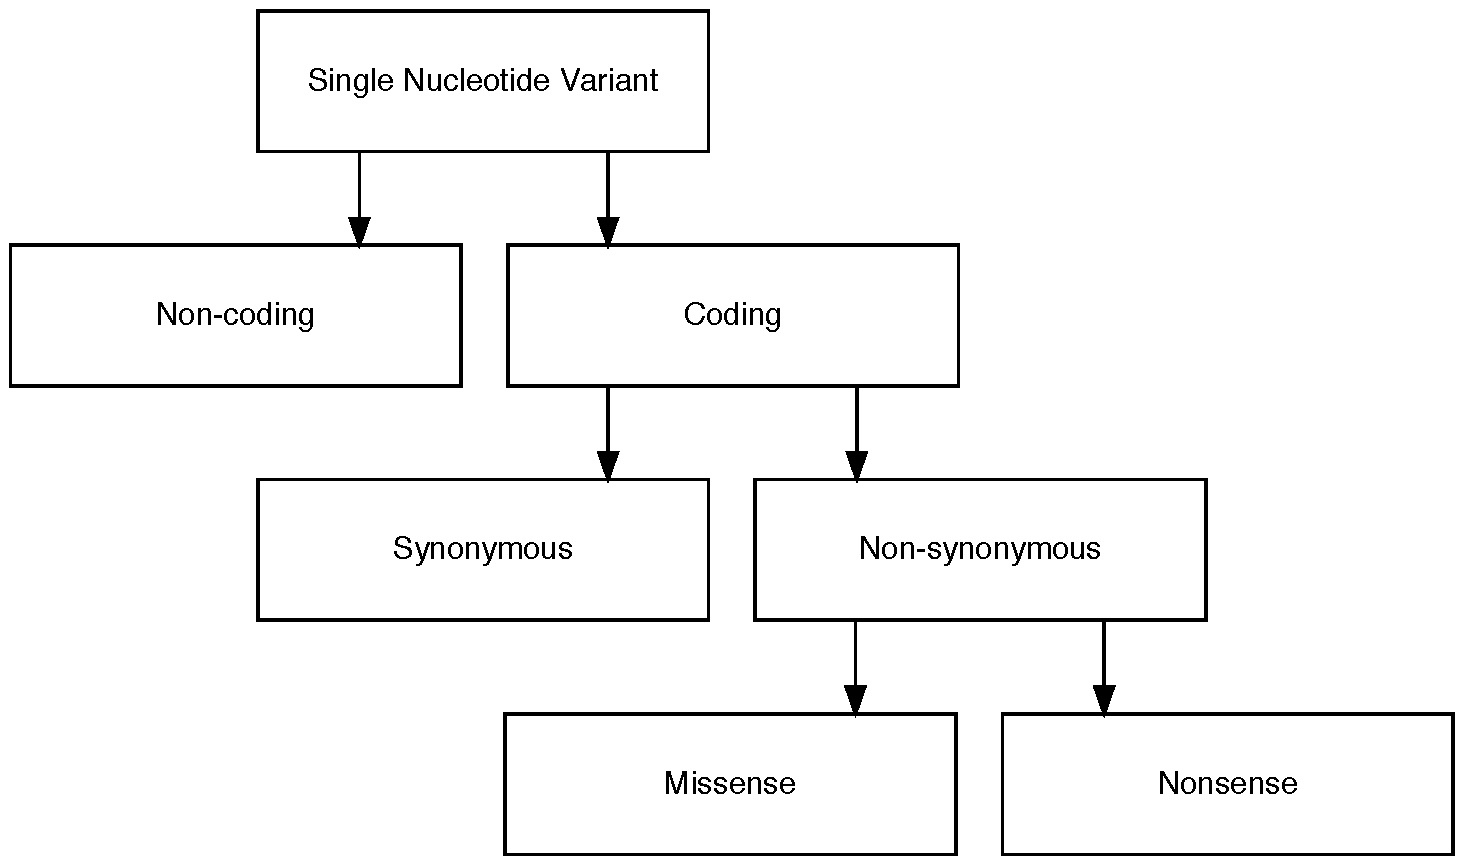
\includegraphics[width=280pt]{img/snv_classification.pdf}
\caption[SNV Classification]{Classification of single-nucleotide variants (SNVs).}
\label{fig:snv-classification}
\end{figure}

While non-synonymous mutations have long been in the spotlight of research, non-coding and synonymous variants have been understudied. However, increasing evidence suggests that both have measurable impact on oncogenesis. Non-coding variants have been found to act as drivers across cancer types~\cite{Rheinbay:2020}. Synonymous mutations, which have been thought to be silent, may play an important role both in the normal genome~\cite{Lebeuf-Taylor:2019} and in cancer~\cite{Supek:2014, Sharma:2020}. While not directly altering protein amino acid sequences, they can affect splicing and expression regulation and may exert a driving effect in this way.


\subsection{Short Insertions and Deletions}

Short insertions and deletions (indels) are small, ≤50bp, genomic alterations. If the number of inserted or deleted bases is divisible by three (the length of a codon) the indel is in-frame, otherwise it is classified as frame-shift since it changes the reading frame. Frame-shift indels are common cancer mutations, particularly in tumor suppressor genes, where they disrupt transcription by inducing premature stop codons. By comparison, in-frame indels are generally less disruptive but still lead to protein alterations that may affect normal function.


\subsection{Structural Variants, Copy Number Variants, and Gene Fusions}

Structural variants (SV) are genomic changes that rearrange the sequence of one or two chromosomes and have a size of >50bp \cite{Alkan:2011}. Rearrangements can occur within one chromosome (intra-chromosomal rearrangements) or between two chromosomes (intra-chromo\-somal rearrangements). Unbalanced SVs affect copy-number relative to the reference genome, meaning gain or loss of genetic loci, and are referred to as copy-number variants (CNVs). CNVs can be insertions, deletions, or duplications \cite{Feuk:2006}. These are common in cancer, where they can lead to overexpression of oncogenes such as \textit{ERBB2} due to increased gene dosage which then drives tumor-growth. Compared to CNVs, simple inversions and translocations are copy-number neutral, although translocations are often complex and associated to copy number changes.

Gene fusions are consequences of SVs, where one or both break ends of an SV lie in a genic region, resulting in a new in-frame gene configuration. Gene fusions are common in many cancers and can be important driver mutations. The best known example is the \textit{BCR}-\textit{ABL1} fusion gene resulting from a translocation between chromosomes 22 and 9, that is common in chronic myelogenous leukemia (CML) and acute lymphobastic leukemia (ALL).

In contrast to SNVs that develop continuously during the lifetime of a tumor, many SVs largely occur early in tumor development during the ``telomere crisis''~\cite{Alkner:2015, Tang:2015}. Individual SVs can be part of complex structural events such as chromothripsis, which describes a single catastrophic chromosomal shattering event followed by incorrect DNA repair~\cite{Stephens:2011}. Since then, other recurring complex events have been described, each having their own signature of structural events~\cite{Nik-Zainal:2012b, Baca:2013, Hadi:2020}. Due to their early occurrence, SVs are ideal biomarkers as many tumor clones will share them. This can be exploited in early detection of disease recurrence~\cite{Olsson:2015}.


\subsection{Epigenetics}

Epigenetic changes are those that do not involve alteration of the DNA nucleotide sequence and play a major role in tumor development~\cite{DawsonKouzarides:2012}. Several types of epigenetic alterations exist, including promoter hyper- and hypomethylation and histone modifications. Promoter hypermethylation has a major influence on transcription dynamics through its ability to silence genes, while hypomethylation has the opposite effect and can lead to increased transcription. Examples in cancer are \textit{BRCA1} and \textit{PTEN} hypermethylation, where transcriptional silencing leads to loss of protein expression, contributing to oncogenesis. Histone modifications are addition or loss of functional groups from histone proteins, performed by certain enzymes. Histones are a principal determinant of chromatin openness and transcription, and alteration of modifications can adversely affect transcription of genes wound around an affected histone.


\subsection{Mutational Signatures}

The mutational processes that shape the tumor genome often generate tell-tale ``signatures'' of mutation type combinations in the genome. Alexandrov \textit{et al}~\cite{Alexandrov:2013} first employed non-negative matrix factorization (NMF) to describe a variety of signatures covering SNVs, their immediate neighbor bases (``sequence context''), and indels across 30 cancer types. They could associate 11 signatures with specific causes, such as overactivity of members of the APOBEC family of cytidine deaminases \cite{Burns:2013}, or exposure to ultraviolet light. Since then, the original signatures have been refined and dozens of other signatures, including those derived from SVs and CNVs, have been described~\cite{Alexandrov:2016, Alexandrov:2020, Degasperi:2020}. Importantly, mutational signatures caused by environmental mutagens~\cite{Kucab:2020} and chemotherapies~\cite{Pich:2019} have been catalogued and may shed further light on these factors.


\subsection{Tumor Mutational Burden}

Tumor mutational burden (TMB) is a measure for the overall number of mutations in a tumor, typically normalized by megabase (Mb) of sequence. It has been proposed as a biomarker that may be useful for indicating sensitivity to immunotherapies~\cite{Samstein:2019}. For as-yet incompletely understood reasons, these therapies show heterogeneous response and currently no biomarker is available to reliably predict treatment outcome. TMB is believed to be a surrogate for neoepitope formation, where body-foreign immunogenic peptides are expressed by the tumor. TMB is not without controversy, as many questions around it remain unsolved. They start with how to define TMB, since the number of detected tumor mutations is a function of sequencing experiment setup. Whole genome sequencing (WGS) or whole exome sequencing (WES) will uncover more mutations than a panel targeting few genes, not even considering RNA sequencing (RNA-seq) based TMB which we investigated in study \IV. Another factor is sequencing depth, where sequencing deeper will result in more mutations than sequencing shallow. TMB also varies by tumor site and subtype~\cite{Chalmers:2017}, possibly necessitating different TMB cutoffs to stratify tumors into TMB-low and TMB-high. Efforts to harmonize TMB determination in certain settings and to account for some of these questions are ongoing~\cite{Merino:2020}.

In 2020 the U.S. Food and Drug Administration (FDA) granted approval for pembrolizumab in TMB-high solid tumors, where the TMB cutoff was defined as ≥10 mut/Mb. This is the first FDA drug approval that allows TMB as a biomarker and, given the questions around TMB, this decision was highly controversial with voices both for~\cite{Subbiah:2020} and against~\cite{PrasadAddeo:2020}. Adding to the controversy, a reanalysis of public clinical study datasets suggests that TMB is in fact not a good marker of response to immune checkpoint blockage~\cite{Gurjao:2020}, but that the supposed signal was a statistical artifact. It has been proposed that it may not the overall mutational burden, but only indels that trigger mRNA nonsense mediated decay that signal response to immunotherapy~\cite{Lindeboom:2019, Litchfield:2020}.


%%%%%%%%%%%%%%%%%%%%%%%%%%%%%%%%%%%%%%%%%%%%%%%%%%%%%%
%
%                 Cancer Transcriptome
%
%%%%%%%%%%%%%%%%%%%%%%%%%%%%%%%%%%%%%%%%%%%%%%%%%%%%%%
\section{The Cancer Transcriptome}

While the genome provides cellular blueprints, the transcriptome represents the dynamic state of the cell. Compared to the genome, the transcriptome is underexplored, perhaps partly due to its inherent complexity. It encompasses the entirety of cellular transcripts (RNAs), the most important and basic element of which is messenger RNA (mRNA). Through transcription from a single gene precursor mRNA is produced, which, through alternative splicing and alternative polyadenylation~\cite{DiGiammartino:2011, Xue:2018}, may be processed into a variety of mature mRNA isoforms. Adding to this, a variety of non-coding RNAs exist, such as transfer RNA (tRNA), microRNA (miRNA), Piwi-interacting RNA (piRNA), vault RNA (vtRNA), and others. These do not code for proteins, but may have functional interactions with each other, with DNA, with mRNA, or with proteins, leading to a complex and dynamic interaction network that is difficult to grasp. Another level of complexity is added by the epitranscriptome, a collection of more than 170 types of RNA editing and modifications, such as deamination of adenosine to inosine (A-to-I editing), methylation of adenosine to N\textsuperscript{6}-methyladenosine (m\textsuperscript{6}A modification), or pseudouridine~($\psi$), that can modulate gene expression levels, protein translation, and localization~\cite{ZhaoHe:2015, Davalos:2018, BooKim:2020, WienerSchwartz:2020}. Lastly, cellular processes, such as nonsense-mediated decay, impact gene expression levels. This may happen by removing mRNAs that contain premature stop codons, for example induced by transcription errors or small DNA indels. 

Compared to the normal transcriptome, the cancer transcriptome is dysregulated due to changes in transcriptomic processes that alter the delicate and complex balance of the transcriptome. Indeed, all known transcriptomic features and processes have been implicated in tumor development when dysregulated, such as gene expression~\cite{Perou:2000, Ross:2000}, alternative splicing~\cite{Kahraman:2020, CherryLynch:2020, Bonnal:2020} and intron retention~\cite{Monteuuis:2020}, and alternative polyadenylation~\cite{Erson-BensanCan:2016}, non-coding RNAs~\cite{SlackChinnaiyan:2019, Rheinbay:2020, Liu:2020}, RNA editing and modifications~\cite{Eisenberg:2018-A-to-I, BarbieriKouzarides:2020, DongCui:2020}, and transcriptomic pathways~\cite{PoppMaquat:2018, Lindeboom:2019}.

The properties of the transcriptome as mediator between DNA and proteome make it an interesting target for diagnostics. It contains information currently diagnostically exploited on the DNA level, provides a wealth of information that can only be probed on the transcriptome level, and through mRNA expression and modifications has direct impact on the proteome.


%%%%%%%%%%%%%%%%%%%%%%%%%%%%%%%%%%%%%%%%%%%%%%%%%%%%%%
%
%                 Breast Cancer
%
%%%%%%%%%%%%%%%%%%%%%%%%%%%%%%%%%%%%%%%%%%%%%%%%%%%%%%
\section{Breast Cancer}

Breast cancer is the most common form of cancer in women. It mostly originates in the duct tissue (\textasciitilde80\%, ductal carcinoma) and lobules (\textasciitilde20\%, lobular carcinoma) of the breast~\cite{Harbeck:2019}, depicted in Figure~\ref{fig:breast-anatomy}. It is inherently heterogeneous, with multiple subtypes that have distinct genetic, phenotypic, and clinical presentations that translate into differing prognosis, risk profiles, and susceptibility to treatments. Although the disease can occur in both women and men, approximately 99\% of patients are female \cite{Ferzoco:2016}. While there are many commonalities in the disease between women and men, considerable differences exist in terms of genetics and clinical characteristics \cite{Nilsson:2011, Johansson:2011, Johansson:2013}. This thesis focuses exclusively on breast cancer in women, and the term ``breast cancer'' in this thesis will from here on only refer to the disease affecting women. Compared to other cancer types, considerable progress has been made in breast cancer diagnosis, treatment, and subsequent patient survival in the last four decades~\cite{Hortobagyi:2020}.

% Breast physiology
% https://www.teresewinslow.com/#/breast/
\begin{figure}[t]
\centering

\includegraphics[width=\textwidth]{img/placeholder.png}
\caption[Anatomy of the Female Breast]{Anatomy of the female breast. Highlighted are the lymph nodes, nipple, areola, muscles, chest wall, ribs, fatty tissue, as well as lobules and ducts.}
\floatfoot{For the National Cancer Institute \copyright{} 2011 Terese Winslow LLC, U.S. Government has certain rights. \\ Reproduced with permission from the copyright holder.}
\label{fig:breast-anatomy}
\end{figure}


\subsection{Incidence and Mortality}
\label{subsec:incidence}

Breast cancer is the most common kind of cancer worldwide accounting for nearly 2.1 million newly diagnosed cases and nearly 630,000 deaths in 2018~\cite{Bray:2018}. This is 11.6\% of all new cancer cases and 24.2\% of cases in women.

There are substantial regional differences in global breast cancer incidence, visualized using data from the World Health Organization for 2018 in Figure~\ref{fig:incidence}. Incidence is age-standardized to account for the varying age structure between populations. Western societies have the highest incidence, largely influenced by lifestyle and dietary choices.

\begin{figure}[t]
\centering
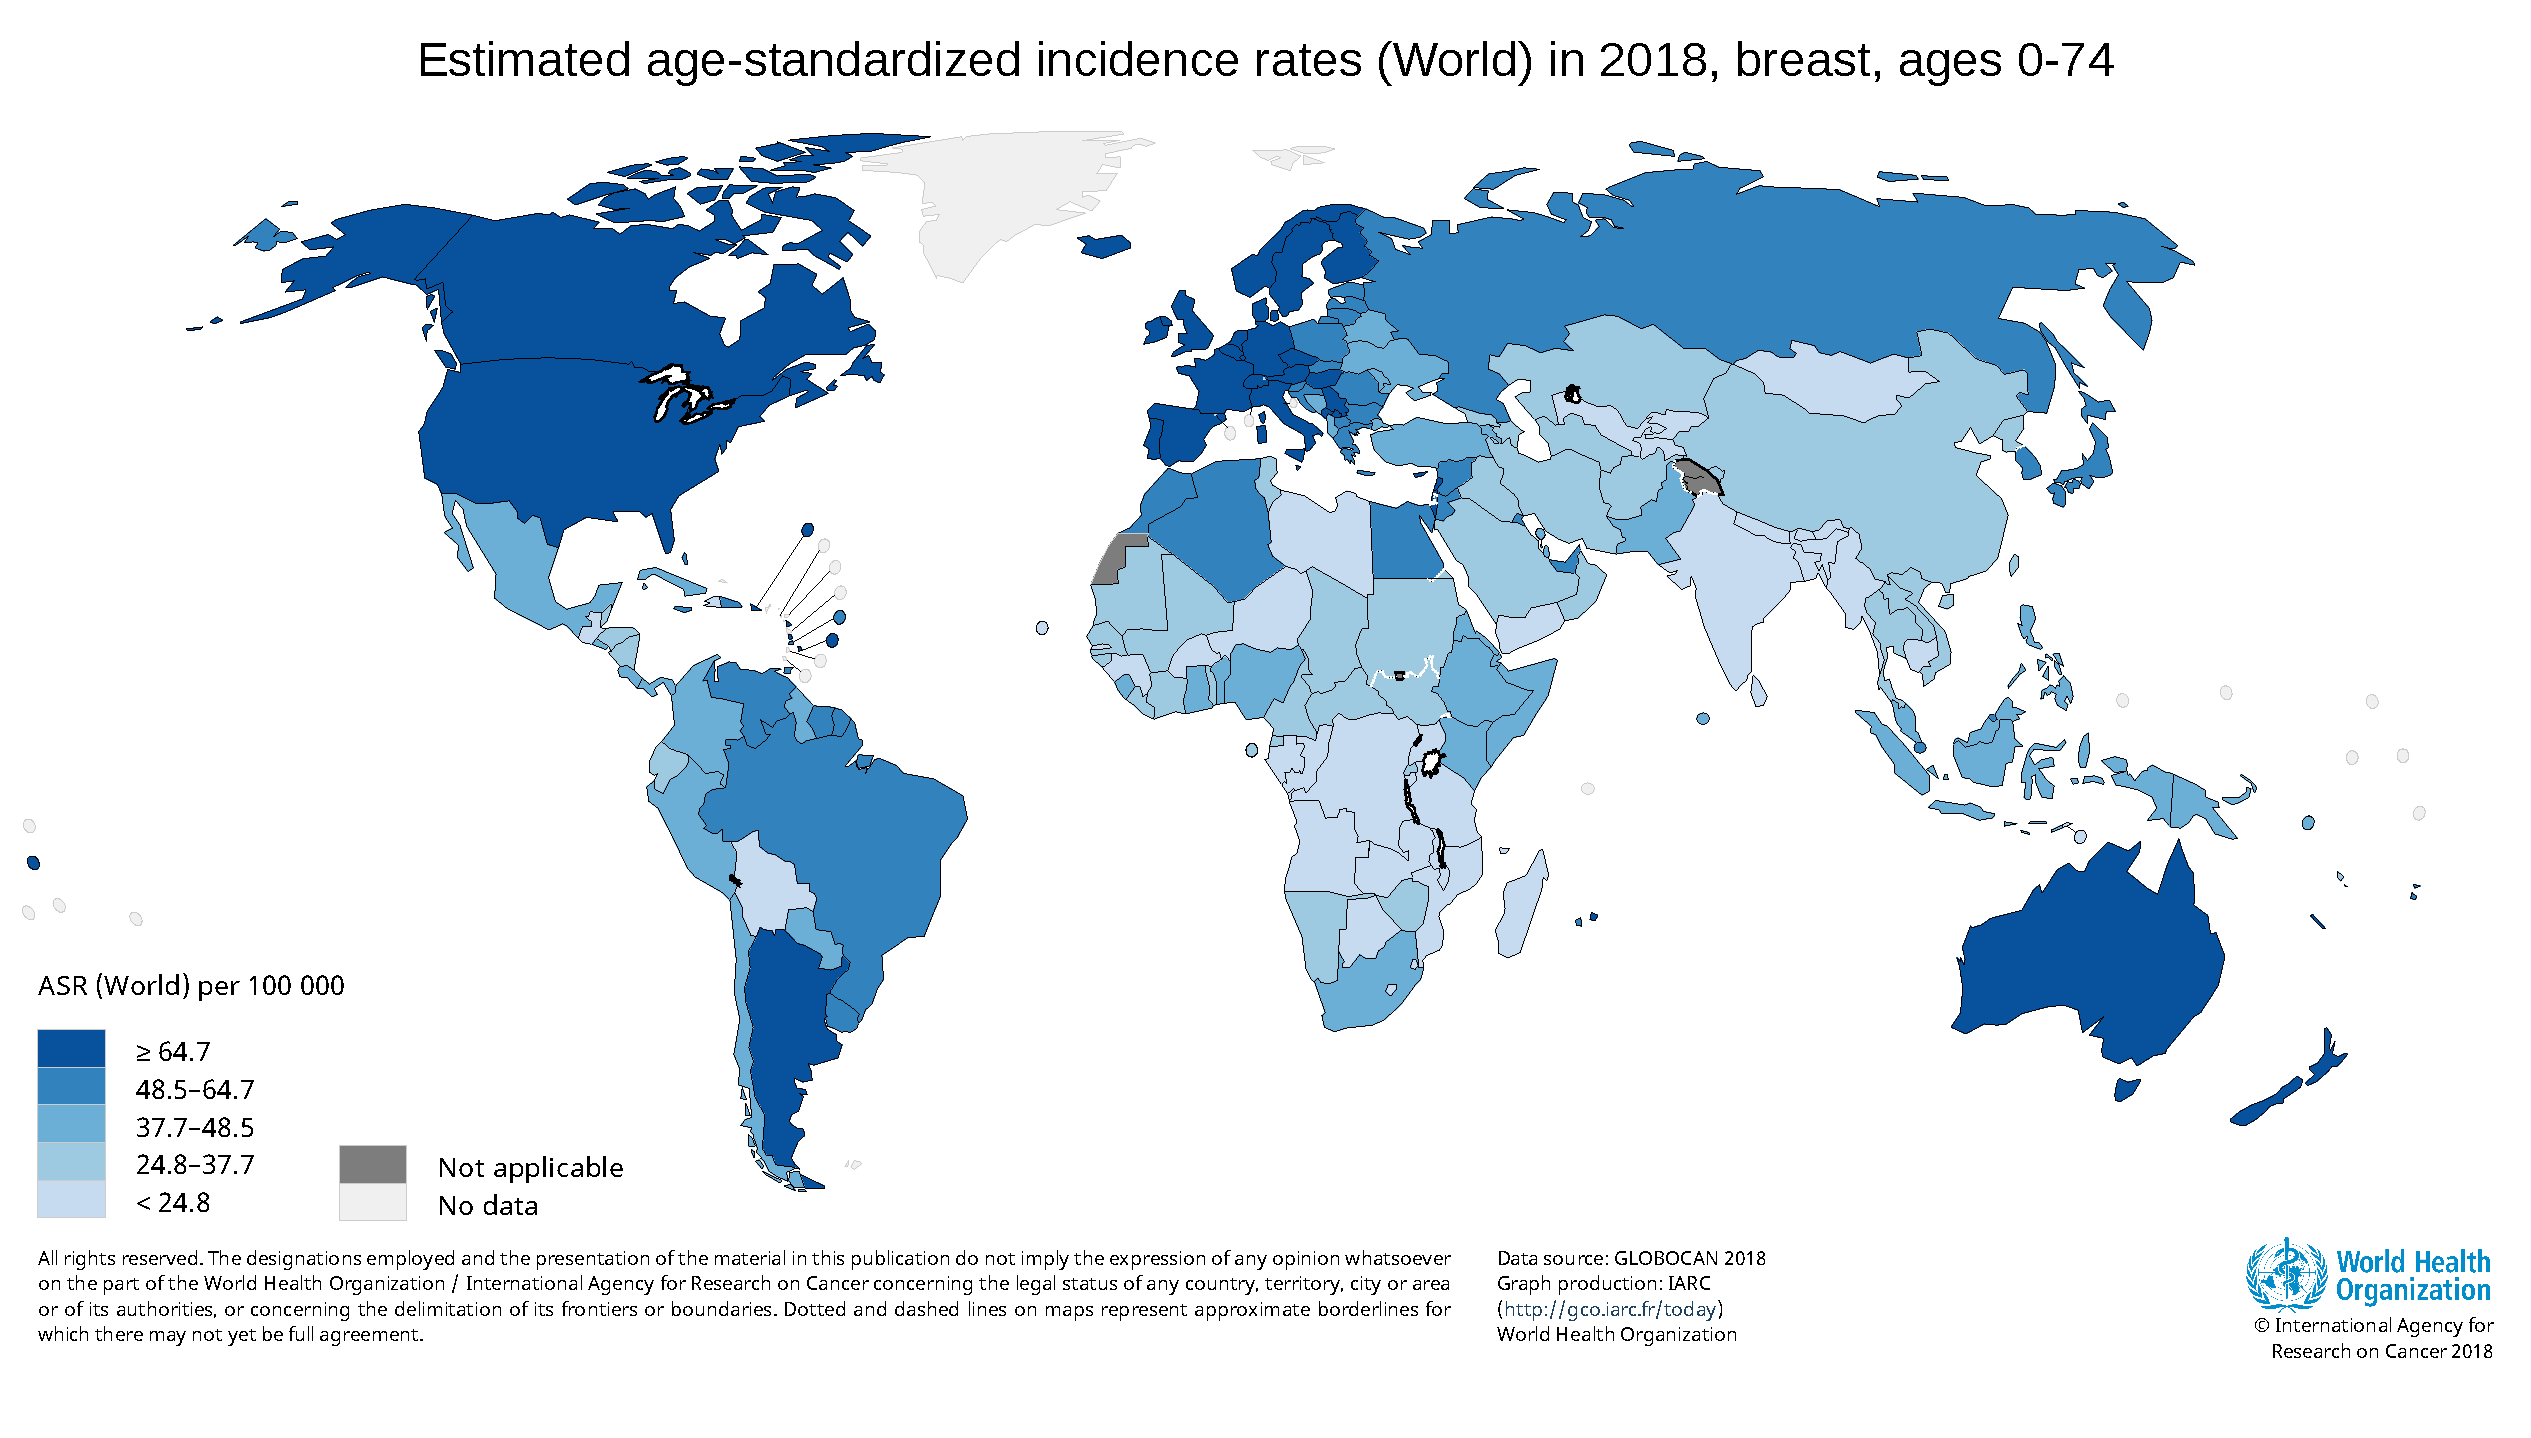
\includegraphics[width=\textwidth, trim={0 35mm 15mm 15mm}, clip]{img/who_incidence_2018.pdf}
\caption[Global Breast Cancer Incidence]{Global estimated age-standardized incidence rate (ASR) for breast cancer per 100,000 women for the year 2018.}
\floatfoot{Source: World Health Organization Global Cancer Observatory (\url{https://gco.iarc.fr})}
\label{fig:incidence}
\end{figure}

In 2018, 30,511 women in Sweden were diagnosed with cancer, of which 7,558 women were diagnosed with breast cancer and 1,391 women succumbed to the disease. This makes breast cancer the second most deadly type of cancer in Sweden behind lung cancer~\cite{socialstyrelsen-2018}. Despite the large number of total deaths, patient survival is generally very good in the short (98\% 1-year survival) to mid-term (88.5\% 5-year survival) compared to other types of cancer. However, 5-year survival cannot be considered a cure, and survival rates significantly decline in the long and very-long term (60\% 15-year survival, 50\% 20-year survival), as patients experience recurrence of their disease~\cite{Brenner:2002, Pan:2017}.

Breast cancer is the most common type of cancer in women and, in Sweden, is the most deadly second only to lung cancer. 


%%%%%%%%%%%%%%%%%%%%%%%%%%%%%%%%%%%%%%%%%%%%%%%%%%%%%%
%
%                 Risk Factors
%
%%%%%%%%%%%%%%%%%%%%%%%%%%%%%%%%%%%%%%%%%%%%%%%%%%%%%%
\subsection{Risk Factors}
\label{subsec:riskfactors}

A diverse range of factors have been identified that increase women's life-time risk of developing breast cancer. Age is the most important risk factor, as mutations accumulate in normal cells over time. In 2018 in Sweden, only 4\% of invasive breast cancers were diagnosed in women under the age of 40 \cite{socialstyrelsen-db}. Breast cancer risk, particularly in postmenopausal women, is modulated by factors that alter endogenous sex hormone levels. High baseline hormone levels, oral contraceptives, early menarche, late menopause, and most hormonal replacement therapies during menopause increase breast cancer risk~\cite{Hamajima:2012, Morch:2017, CGHFBC:2019}. Additionally, reproductive aspects such as parity, age at first childbirth, the number of children, and breast feeding have complex effects on breast cancer risk~\cite{Ewertz:1990}.

A variety of dietary and lifestyle factors have been found to increase breast cancer risk: consumption of alcohol~\cite{Romineu:2015, Garaycoechea:2018} and processed meat~\cite{Inoue-Choi:2016, Anderson:2018}, as well as active and passive exposure to tobacco smoke \cite{Dossus:2014}. Obesity and high body fat content, both measured as body-mass index (BMI) and in a BMI-independent way~\cite{Pearson-Stuttard:2018, Iyengar:2018, Bjorge:2019}, as well as lack of exercise~\cite{Friedenreich:2010, Wu:2013} are associated with higher risk. Lastly, exposure to environmental factors such as ionizing radiation, including X-radiation and gamma radiation, elevates risk.

A particularly important risk factor is a family history of cancer as approximately 5\%--10\% of breast cancers are hereditary. The mechanism of action is thought to be Knudson's two-hit hypothesis~\cite{Knudson:1971}, whereby patients have inherited a damaged copy of a risk gene from their parents (first hit), and the second copy is damaged during the person's lifetime leading to loss of heterozygosity (LoH), for example by exposure to environmental carcinogens (second hit). Approximately 25\% of all hereditary cases can be explained by high-risk variants in the \textit{BRCA1} and \textit{BRCA2} genes~\cite{Nielsen:2016}. Rare germline mutations in other high-penetrance genes cause specific forms of breast cancer, the most prominent being 
\textit{PTEN} hamartoma tumor syndrome caused by \textit{PTEN} variants, and Li-Fraumeni syndrome caused by \textit{TP53} variants. The remaining cases can be partly attributed to variants in medium to low risk genes including \textit{CHEK2}, \textit{PALB2}, \textit{RAD50}, \textit{ATM}, and \textit{BARD1}. However, a proportion of cases cannot be explained by the risk genes known to date. In Sweden, breast cancer risk variants are being explored through initiatives such as the SWEA study, and efforts to identify unknown risk variant carriers through studies such as BRCAsearch~\cite{Nilsson:2018}. In all hereditary cases genetic counseling is imperative to guide possible prophylactic measures such as mastectomy and/or oophorectomy, and to determine whether the patient's relatives may carry the risk alleles.


%%%%%%%%%%%%%%%%%%%%%%%%%%%%%%%%%%%%%%%%%%%%%%%%%%%%%%
%
%                 Diagnosis
%
%%%%%%%%%%%%%%%%%%%%%%%%%%%%%%%%%%%%%%%%%%%%%%%%%%%%%%
\subsection{Diagnosis}
\label{subsec:diagnosis}

Breast cancer is most often detected either through early detection techniques such as mammographic screening, or self-examination of the breasts by the patient. While mammographic screening has led to early detection of many breast cancers~\cite{Duffy:2020}, it is not without controversy as it can also lead to overdiagnosis~\cite{Loberg:2015}. It is predicted that a significant number of detected lesions may never become invasive during the patient's lifetime, however we currently lack the tools to detect which ones. On the other hand, current screening methods can miss lesions, for example due to lobular phenotype of the lesion \cite{Johnson:2015}, or due to high breast density \cite{VourtsisBerg:2018}.

To guide treatment decisions, tumor biopsy and surgery samples are evaluated using histopathological and/or genomic methods and classified by their morphological, clinicopathological, and genomic features. The most important classification schemes are described in the following sections.


%%%%%%%%%%%%%%%%%%%%%%%%%%%%%%%%%%%%%%%%%%%%%%%%%%%%%%
%
%                 Classification
%
%%%%%%%%%%%%%%%%%%%%%%%%%%%%%%%%%%%%%%%%%%%%%%%%%%%%%%
\subsection{Classification}
\label{subsec:classification}

Several systems exist to class tumors into prognostic and treatment-predictive subgroups. These include systems based on histopathology such as Nottingham histological grade (NHG) and TNM stage, and molecular methods based on gene expression signatures.


\subsubsection{Histopathology}

% Kumar:2009: https://books.google.se/books?id=mwD5Y0jMUZAC&pg=PA1084#v=onepage&q&f=false
Between 15\% and 30\% of breast tumors are \textit{in situ} carcinomas; that is, the tumor cell growths have not broken through the basement membrane layer. These are often detected using screening programs and consequently the exact percentage of \textit{in situ} tumors depends on the prevalence of screening in the population. Based on the site of origin one can differentiate ductal carcinoma \textit{in situ} (DCIS,~\textasciitilde80\%) and lobular carcinoma \textit{in situ} (LCIS,~\textasciitilde20\%)~\cite{Kumar:2009}. Most \textit{in situ} carcinomas are benign, but some harbor malignant potential and may or may not become invasive if left untreated. One of the major challenges is improving diagnostics to enable this distinction.

Invasive carcinomas constitute between 70\% and 85\% of all breast cancers. The majority of these are invasive ductal carcinomas (IDC, \textasciitilde79\%) of not otherwise specified (NOS) type, followed by invasive lobular carcinomas (ILC, \textasciitilde10\%). The remaining cases can be further stratified based on cytological features into tubular~(\textasciitilde2\%), medullary (\textasciitilde5\%), mucinous~(\textasciitilde2\%), papillary~(1\%-2\%), and cribriform~(0.8\%-3.5\%) cancer~\cite{Makki:2015}.


\subsubsection{Grade}

Nottingham histological grade according to the Elston and Ellis modified Scarff-Bloom-Richardson system (NHG) is a morphological marker that describes how closely tumor cells resemble normal breast epithelial cells~\cite{ElstonEllis:1991}. Generally with increasing grade, resemblance to normal cells decreases and tumor aggressiveness is thought to increase. NHG is a compound score consisting of the three morphologic components tubular differentiation, number of mitoses, and nuclear pleomorphism. The component-scores are determined individually for a tumor, added together, and categorized according to Table~\ref{tab:nhg-scoring}. NHG is a strong prognostic factor in breast cancer~\cite{Rakha:2008}, however it has long had reproducibility problems~\cite{Rakha:2010} which we also observed in study~\III.

\begin{table}[t]
\centering
\caption[Nottingham Histological Grade]{Nottingham histological grade scoring and interpretation.}
\label{tab:nhg-scoring}
\begin{tabular}{ ccl }
\toprule
Score & Grade & Interpretation \\
\midrule
3--5 & 1 & well differentiated \\
6--7 & 2 & moderately differentiated \\
8--9 & 3 & poorly differentiated \\
\bottomrule
\end{tabular}
\floatfoot{Source: Elston \& Ellis \cite{ElstonEllis:1991}}
\end{table}


\subsubsection{Stage}

Pathologic stage describes how advanced a cancer is. The TNM system is the most widely used staging system in breast cancer. It was originally proposed by Denoix in 1946~\cite{Denoix:1946} and today is maintained by the Union for International Cancer Control (UICC) and the American Joint Committee on Cancer (AJCC). The TNM system classifies cancer by the size of the tumor (T), the number of lymph nodes containing tumor cells (N), and metastatic spread (M). Each of these categories has subcategories, such as T1--T4 for increasing tumor size, that describe the extent of disease progression. In the simplest use, the stage group is then determined using only the T, N, and M subcategories according to Table~\ref{tab:stage}. Stage grouping can be made more fine grained by incorporating additional information such as prefix modifiers describing the information source and may be modified by NHG, histological receptor status, and the score of the Oncotype DX genomic assay (see Section~\ref{subsec:signatures}).

%
% Stages: https://cancerstaging.org/references-tools/deskreferences/Documents/AJCC%20Cancer%20Staging%20Form%20Supplement.pdf
%
\begin{table}[t]
\centering
\caption[TNM Staging]{Pathologic stage as defined by the 8th edition of the AJCC TNM system description using only the mandatory parameters T, N, and M.}
\label{tab:stage}
\begin{tabular}{ cll }
\toprule
Stage & TNM Categories & Interpretation \\
\midrule
\multirow{1}{*}{0}   & Tis N0 M0      & \multirow{1}{*}{pre-invasive stage} \\[4pt]
\multirow{3}{*}{I}   & T1 N0 M0       & \multirow{3}{*}{low stage} \\
                     & T0 N1mi M0     & \\
                     & T1 N1mi M0     & \\[4pt]
\multirow{6}{*}{II}  & T0 N1 M0       & \multirow{6}{*}{intermediate stage} \\
                     & T1 N1 M0       & \\
                     & T2 N0 M0       & \\
                     & T2 N1 M0       & \\
                     & T3 N0 M0       & \\[4pt]
\multirow{9}{*}{III} & T0 N2 M0       & \multirow{9}{*}{high stage} \\
                     & T1 N2 M0       & \\
                     & T2 N2 M0       & \\
                     & T3 N1 M0       & \\
                     & T3 N2 M0       & \\
                     & T4 N0 M0       & \\
                     & T4 N1 M0       & \\
                     & T4 N2 M0       & \\
                     & Any T N3 M0    & \\[4pt]
\multirow{1}{*}{IV}  & Any T Any N M1 & \multirow{1}{*}{metastatic stage} \\
\bottomrule
\end{tabular}
\floatfoot{Source: AJCC Cancer Staging Manual \nth{8} Ed. \cite{AJCC:2018}}
\end{table}


\subsubsection{Receptor Status}

The expression status of the receptor proteins estrogen receptor (ER), progesterone receptor (PR or PgR), and human epidermal growth factor receptor 2 (HER2) is routinely determined using immunohistochemistry (IHC) for breast tumors and is of prime importance for prognosis and treatment (see Section~\ref{subsec:treatment}). Tumor slides are stained for these receptors using antibodies. Stained cells are counted or estimated versus non-stained cells, resulting in a stained cell percentage. Receptor status is dichotomized into positive/negative status based on a cutoff. In Sweden for ER/PgR, a cutoff of 10\% stained cells is used, while internationally a cutoff of 1\% is common. For HER2, an additional \textit{ERBB2} gene copy-number analysis using fluorescence or silver \textit{in situ} hybridization (FISH or SISH) is recommended if the HER2 IHC result is inconclusive. Recently, a new subgroup of HER2-low has been proposed to mark tumors with low HER2 protein expression and no \textit{ERBB2} gene amplification that would traditionally be called HER2-~\cite{Tarantino:2020}. Increasing evidence suggests that a subset of these tumors may benefit from HER2 targeting agents.

By combining ER, PgR, and HER2 status, tumors can be categorized into clinical subgroups, whereby ER and PgR may be summarized into hormone receptor (HoR\footnote{A more common abbreviation for hormone receptor is HR, however this abbreviation is also commonly used for the Hazard Ratio. We therefore opted for abbreviating hormone receptor as HoR in studies \III, \IV, and in this thesis.}) status. Patients with HoR+ tumors have a better survival rate than those with HoR- tumors~\cite{Bentzon:2008}. This includes the HoR+/HER2- group, which constitutes the largest subgroup with 68\% of cases in the U.S. between 2013 and 2017 \cite{seer-db}, and generally has the best prognosis~\cite{PariseCaggiano:2014} followed by HoR+/HER2+ tumors (\textasciitilde10\%). Compared to these HoR+ groups, survival of patients with HoR-/HER2+ (\textasciitilde4\%) is significantly worse. Triple-negative breast cancer (TNBC, \textasciitilde10\%) lacks expression of all three receptors, and thus offers no molecular targets for the most common targeted agents. Consequently it has the worst prognosis, with chemotherapy being the only treatment option.


\subsubsection{Intrinsic Subtypes}

In addition to classing tumors by morphology and histology, they can be stratified by their intrinsic subtype. These define distinct groups of tumors with similar gene expression patterns and clinical characteristics. Molecular subtypes were first discovered by Perou and Sørlie \textit{et al} \cite{Perou:2000} who performed unsupervised hierarchical clustering on the global gene expression profiles of normal tissues and breast tumor tissues from 42 patients. The subtypes were quickly found to be prognostic~\cite{Sorlie:2001}. The originally reported subtypes Luminal-like, Basal-like, HER2-enriched, and Normal-like were later refined by differentiating the Luminal-like group into Luminal A-like and Luminal B-like tumors~\cite{Sorlie:2003}. More recently the Claudin-low subtype has been defined~\cite{Herschkowitz:2007}, although its status as a true intrinsic subtype has been disputed~\cite{Fougner:2020}. The subtypes have been reproduced numerous times across technology platforms~\cite{Hu:2006, Picornell:2019} and in metastatic tumors~\cite{Weigelt:2005, Tobin:2015, Prat:2016-met, Cejalvo:2017}. They also exhibit distinct methylation patterns~\cite{Holm:2010}.

The Luminal- and Basal-like subtypes were originally named due to the similarity of their gene expression patterns to normal luminal and basal epithelial cells. In the Luminal-like case this is a gene expression signature reflecting estrogen receptor activation. The Luminal A-like subtype is characterized by a normal HER2 expression profile and low activity of proliferation genes, while Luminal B-like tumors show elevated proliferation and can have \textit{ERBB2} overexpression. The Basal-like subtype is characterized by a gene expression signature including activation of basal keratins, integrin-$\beta$4, and laminin. The HER2-enriched subtype features a signature of \textit{ERBB2} overactivation~\cite{Perou:2000}. Samples of Normal-like subtype typically cluster together with true normal breast tissue samples. The existence of Normal-like as a true intrinsic subtype has been questioned as it is possibly a technical artifact caused by samples with low tumor cell content~\cite{Peppercorn:2008, Parker:2009, PratPerou:2011}. It is therefore sometimes omitted from analysis.

Since expression profiling remains a non-standard diagnostic tool, surrogate intrinsic subtypes can be derived from traditional clinicopathological biomarkers in combination with Ki67 protein status as a surrogate marker for proliferation, and NHG using the St. Gallen classification schema~\cite{Goldhirsch:2013}. NHG may also be useful in refining the classification, particularly for differentiating between Luminal A-like and B-like tumors~\cite{Curigliano:2017-deescalation, Ehinger:2017}. However, concordance between expression-based subtypes and surrogate subtypes is generally poor~\cite{Guiu:2012, Prat:2015-subtyping, Lundgren:2019}, and thus the surrogate classification remains an imperfect stopgap solution until expression profiling is integrated into the clinical routine.

In addition to aiding our understanding of breast cancer biology, the introduction of the St. Gallen surrogate subtypes is a testament to the importance and potential clinical impact of the intrinsic subtypes. In particular the intrinsic subtypes are useful in refining the traditional clinicopathological grouping by receptor status, where the groups \mbox{HoR+/HER2-,} HoR+/HER2+, HoR-/HER2+, and HoR-/HER2- show heterogeneous compositions of molecular subtypes~\cite{Parker:2009} with prognostic and treatment-predictive implications~\cite{Rouzier:2005, Rody:2007, Prat:2015-subtyping, Prat:2015, Cejalvo:2018}.


\subsubsection{Gene Expression Signatures}
\label{subsec:signatures}

Gene expression signatures provide a dimension to breast cancer classification beyond traditional clinicopathological biomarkers. Based on the expression of a defined number of genes, they capture the transient state of a tumor and are used to define phenotypes such as the intrinsic subtypes and biomarker status, and to predict risk. While a plethora of multi-gene signatures have been developed in the research setting to date, these signatures have shown little gene overlap~\cite{Fan:2006}. Wirapati \textit{et al} performed an early meta-analysis of nine expression signatures across 2,833 tumors and found concordance in terms of signature gene function~\cite{Wirapati:2008}. Their findings were later reproduced and extended by Huang \textit{et al}~\cite{Huang:2018}. More recently, within the \scanb{} study (see Section~\ref{sec:scanb}), 19 gene signatures for subtyping and risk prediction were benchmarked across a large population-based tumor series~\cite{Vallon-Christersson:2019} and found to provide additional prognostic value over traditional clinicopathological classifications in ER+/HER2- disease. However, signatures did not provide further risk stratification in the patient subgroups with ER-/HER2+ and TNBC disease that have particularly bad prognosis. 

% OncotypeDX stage I or II invasive ER+, lymph node negative breast cancer
% MammaPrint stage I or stage II invasive BC smaller than 5cm with up to three positive lymph nodes, irrespective of HR status
% Prosigna: early-stage, hormone-receptor positive disease with up to three positive lymph nodes after 5 years of hormonal therapy treatment.
% EndoPredict stage I or II ER+, HER2-, node-negative breast cancer OR up to three positive lymph nodes \cite{Dubsky:2020}
The clinical implications of risk prediction signatures have been reviewed several times \cite{SotiriouPusztai:2009, Prat:2012, Matikas:2019}, highlighting in particular those signatures that have been commercialized and/or validated in large patient cohorts. The most widely used signatures are the 21 gene signature, commercialized as the Oncotype DX assay (Genomic Health)~\cite{Fisher:1997, Paik:2004, SparanoPaik:2008}, the 70 gene signature commercialized as MammaPrint (Agendia)~\cite{vantVeer:2002}, the PAM50 Risk of Recurrence (RoR) score (which excludes the Normal-like subtype), commercialized as the Prosigna Breast Cancer Prognostic Gene Signature Assay (NanoString Technologies)~\cite{Parker:2009, Wallden:2015}, and EndoPredict (Myriad Genomics). They share approval as risk prediction signatures for early breast cancers that are at risk of developing distant metastases, and thus may be utilized to decide upon adjuvant therapy. Several clinical trials are in progress to validate this potential, including MINDACT (ClinicalTrials.gov identifier \href{https://clinicaltrials.gov/ct2/show/NCT00433589}{NCT00433589}), \mbox{TAILORx} (ClinicalTrials.gov identifier  \href{https://clinicaltrials.gov/ct2/show/NCT00310180}{NCT00310180}), and RxPONDER (ClinicalTrials.gov identifier  \href{https://clinicaltrials.gov/ct2/show/NCT01272037}{NCT01272037}))~\cite{Sparano:2006, Cardoso:2007, Wong:2012}. Early results indicate that gene expression profiling tests can indeed identify low risk patients that may be spared unnecessary treatment~\cite{Cardoso:2016, Stemmer:2017, Sparano:2018}.

Other signatures try to reproduce standard histopathological biomarkers such as receptor status~\cite{Kun:2003, Gruvberger-Saal:2004, Roepman:2009, Bastani:2013, Wilson:2014, Viale:2014, Varga:2017} and NHG \cite{Ivshina:2006, Sotiriou:2006-GG, Ma:2008}. Genomic grade signatures classify tumors into low or high grade, thus clarifying the intermediate NHG class grade 2. Commercial variants of this concept are MapQuant DX (Ipsogen) and Breast Cancer Index (Biotheranostics).

Most commercial gene expression signatures presented here are FDA-approved and were explicitly endorsed by the 2017 St. Gallen conference consensus panel as tools for guiding treatment with adjuvant chemotherapy in node-negative tumors, including MammaPrint, PAM50 RoR, EndoPredict, and Breast Cancer Index.

In Sweden, these tests are not widely used as they are expensive and the cost-benefit ratio has not yet been fully established. Instead, traditional clinicopathological variables and surrogate subtypes are being used for prognostication and definition of treatment regimens. However, increasingly guidelines now do recommend the use of a gene expression risk stratification test, and use of such tests is anticipated to increase dramatically in Sweden in the near future.


%%%%%%%%%%%%%%%%%%%%%%%%%%%%%%%%%%%%%%%%%%%%%%%%%%%%%%
%
%                 Treatment
%
%%%%%%%%%%%%%%%%%%%%%%%%%%%%%%%%%%%%%%%%%%%%%%%%%%%%%%
\subsection{Treatment}
\label{subsec:treatment}

The goal of primary breast cancer treatment is to remove all remnants of the tumor and prevent it from relapsing. The strategy currently recommended by the European Society for Medical Oncology (ESMO) is outlined in Figure~\ref{fig:primary-treatments}. Primary treatment is, in virtually all cases, surgical removal of the tumor, if possible using breast-conserving surgery (BCS). To prevent relapse in the BCS case, additional radiotherapy is crucial to eradicate possible leftover tumor deposits. For tumors that are too large for BCS, neoadjuvant therapy may be attempted to shrink the tumor to a size where BCS is feasible; otherwise, mastectomy is performed. To support primary treatment and reduce the risk of recurrence, adjuvant treatment is recommended.

% https://www.annalsofoncology.org/article/S0923-7534(19)31287-6/fulltext
\begin{sidewaysfigure}

\includegraphics[scale=0.3]{img/placeholder.png}
\caption[ESMO Primary Treatment Algorithm]{Algorithm for primary treatment of early breast cancer by the European Society for Medical Oncology (ESMO). \\
\textbf{a} Biology that requires ChT (TNBC, HER2-positive, luminal B-like), to assess response and prognosis and eventually decide on postoperative
therapies, should preferentially receive preoperative ChT. \\
\textbf{b} Aggressive phenotypes: TNBC or HER2-positive breast cancer. \\
\textbf{c} If ChT is planned, it should all be given as neoadjuvant. \\ 
\textbf{d} Concomitant postoperative RT, postoperative ET and anti-HER2 therapy \\
Abbreviations: BCS -- breast-conserving surgery; ChT -- chemotherapy; ET -- endocrine therapy; HER2 -- epidermal growth factor receptor 2; RT -- radiotherapy; TNBC -- triple-negative breast cancer.}
\floatfoot{Figure and descriptions a--d reprinted from Cardoso \textit{et al} \cite{Cardoso:2019} with permission from Elsevier.}
\label{fig:primary-treatments}
\end{sidewaysfigure}


\subsubsection{Neoadjuvant Treatment}

Neoadjuvant therapies are administered before the primary treatment. They may be used to shrink a tumor down to a size that makes it feasible to perform surgery at all, or less invasive surgery. The neoadjuvant period also provides a window of opportunity for testing how the tumor reacts to therapies before it is surgically removed, potentially proving guidance for adjuvant treatment. This concept is being utilized in clinical trials such as the I-SPY study~\cite{Barker:2009} (ClinicalTrials.gov identifier \href{https://clinicaltrials.gov/ct2/show/NCT01042379}{NCT01042379}).

\subsubsection{Adjuvant Treatment}

Adjuvant treatments are administered after and in support of primary treatment and are guided by biomarkers and clinicopathological features. The current ESMO adjuvant treatment recommendations are outlined in Figure~\ref{fig:adjuvant-treatments}~\cite{Cardoso:2019}. Tumors determined to be HoR+ are treated with targeted anti-hormonal agents such as tamoxifen, or aromatase inhibitors that block estrogen synthesis, such as letrozole. Those showing overexpression of the HER2 receptor protein receive targeted anti-HER2 treatment, for example the monoclonal antibody trastuzumab. All patients with the exception of those with ER+/HER2- (Luminal A-like) disease receive additional chemotherapy, typically anthracycline and taxane. For triple-negative tumors chemotherapy is currently the only first-line treatment option.


% https://www.annalsofoncology.org/article/S0923-7534(19)31287-6/fulltext
\begin{sidewaysfigure}
\centering

\includegraphics[scale=0.3]{img/placeholder.png}
\caption[ESMO Adjuvant Treatment Algorithm]{Algorithm for adjuvant treatment of early breast cancer by the European Society for Medical Oncology (ESMO).\\
\textbf{a} With possible exception of selected cases with very low risk T1abN0.\\
\textbf{b} Anti-HER2: trastuzumab $\pm$ pertuzumab. \\
\textbf{c} Adenoid cystic or apocrine, secretory carcinoma, low-grade metaplastic carcinoma.\\
\textbf{d} Depending on level of ER and PgR expression, proliferation, genomically assessed risk, tumor burden and/or patient preference. \\ 
\textbf{e} Except for very low-risk patients T1abN0 for whom ET/anti-HER2 therapy alone can be considered. \\
Abbreviations: ChT -- chemotherapy; ER -- estrogen receptor; ET --  endocrine therapy; HER2 -- epidermal growth factor receptor 2; N0 -- node negative; PgR -- progesterone receptor; TNBC -- triple-negative breast cancer.}
\floatfoot{Figure and descriptions a--e reprinted from Cardoso \textit{et al} \cite{Cardoso:2019} with permission from Elsevier.}
\label{fig:adjuvant-treatments}
\end{sidewaysfigure}


\subsubsection{Advanced Disease}

Despite primary and adjuvant treatment, tumors can advance or recur even after many years of a patient being disease-free. Often these tumors have developed resistance to standard treatments used in early disease, so different therapies are needed. Recent years have seen several treatment innovations in this area, mostly in combination with other therapies.

% CDK4/6: palbociclib, abemaciclib, ribociclib
In hormone therapy resistant ER+/HER2- breast cancer, CDK4/6 inhibitors are showing promise, for example when combined with selective estrogen receptor degraders (SERDs) such as fulvestrant~\cite{Gao:2020}. In hospitals participating in the \scanb{} study (see section~\ref{sec:scanb}), this type of drug has been used since spring 2017.

Several targeted drugs are being approved or showing strong promise in tumors with specific gene mutations. Approximately one-third of breast tumors have mutations in the \textit{PIK3CA} oncogene. While targeting this gene effectively has long been difficult, recent advances have led to the approval of the PI3K inhibitor alpelisib (Novartis)~\cite{Juric:2018} in \textit{PIK3CA}-mutant HoR+/HER2- disease in combination with fulvestrant~\cite{Andre:2019}. Metastatic tumors often develop therapy resistance to standard treatments such as anti-HER2 drugs prescribed in early disease. Tyrosine kinase inhibitors (TKIs) such as the recently FDA-approved tucatinib can overcome this resistance. Additionally, Poly (ADP-ribose) polymerase (PARP) inhibitors have shown promise in DNA-repair-deficient tumors such as those with \textit{BRCA1} or \textit{BRCA2} mutations.

Another emerging class of drug are antibody-drug conjugates, where traditional antibodies such as trastuzumab are conjugated with a cytotoxic agent. This combination leads to a more targeted release of the traditionally systemically-working cytotoxin by guidance to tumor cells via the antibody. Examples of these drugs include trastuzumab emtansine and trastuzumab deruztecan approved for treatment of advanced HER2+ tumors, and sacituzumab govitecan in advanced TNBC.

Lastly, immunotherapies have shown promise in many types of difficult to treat tumors. In breast cancer, PD-1/PD-L1 inhibitors such as atezolizumab and pembrolizumab are being used to treat metastatic tumors and triple-negative tumors~\cite{Marra:2019}. Beyond PD-1 checkpoint blockage approaches, tumor infiltrating lymphocytes have shown promise in select cases~\cite{Zacharakis:2018}, and other options have been reviewed by Chrétien \textit{et al}~\cite{Chretien:2019}. However, immunotherapies come with their own risks and are prone to causing a wide range of immune-related adverse events such as cytokine storms~\cite{Postow:2018} and elevated risk for developing secondary cancers~\cite{Wartewig:2017, LudinZon:2017}. Additionally it remains unclear which patients benefit from immunotherapy and there is a lack of biomarkers predictive of treatment success.


%%%%%%%%%%%%%%%%%%%%%%%%%%%%%%%%%%%%%%%%%%%%%%%%%%%%%%
%
%                 Breast Cancer Genomics
%
%%%%%%%%%%%%%%%%%%%%%%%%%%%%%%%%%%%%%%%%%%%%%%%%%%%%%%
\subsection{Molecular Landscape}
\label{subsec:breast-cancer-genomics}

Breast cancers are driven by unique genomic and transcriptomic properties. Large-scale high-throughput sequencing initiatives including The Cancer Genome Atlas (TCGA), the Molecular Taxonomy of Breast Cancer International Consortium (METABRIC), the International Cancer Genome Consortium (ICGC) \cite{ICGC:2010}, and others have thoroughly mapped the genomic landscape of both early and advanced breast cancer in the past decade~\cite{Sjoblom:2006, Curtis:2012, TCGA-Breast:2012, Nik-Zainal:2016, Pereira:2016, Staaf:2019, Campbell:2020}. Others have explored the clonal evolution of breast tumors~\cite{Nik-Zainal:2012a, Shah:2012, Yates:2015}.

On average, breast tumors have a low to medium mutation burden compared to other cancer types such as melanoma~\cite{Chalmers:2017, Alexandrov:2013, Kandoth:2013, Campbell:2020}. The landscape in early breast cancer is dominated by mutations in the genes \textit{PIK3CA} and \textit{TP53}. The oncogene \textit{PIK3CA} is mutated in \textasciitilde35\% of breast tumors, and features a wide spectrum of missense mutations that lead to overactivation of growth signalling via the PI3K-AKT-mTOR pathway. This includes the most common mutation in breast cancer, \textit{PIK3CA} H1047R~\cite{TCGA-Breast:2012, Martinez-Saez:2020}. The tumor suppressor gene \textit{TP53} on the other hand is frequently disrupted by dominant-negative point mutations, frame-shift indels, and nonsense mutations that trigger nonsense-mediated decay of the incomplete \textit{TP53} transcripts.

Copy-number alterations play a major role in breast cancer. Particularly the locus 17q11 around the oncogene \textit{ERBB2} is frequently amplified, which has lead to the adoption of HER2 testing to guide treatment with anti-HER2 therapy. Further recurrently amplified loci are 8q11, 8q13, and 8q24 on chromosome 8, as well as 17q23 and 20q13, involving genes such as \textit{MYC}~\cite{TCGA-Breast:2012}. Other loci are frequently disrupted or lost entirely, such as those involving \textit{PTEN}~\cite{Saal:2008} and \textit{RB1} \cite{Jonsson:2012}. Other SVs are common~\cite{Stephens:2009} and genomic SV hotspots exist~\cite{Fimereli:2018}, but recurrent SVs and gene fusions are rare~\cite{Edgren:2011, Robinson:2011, Banerji:2012, Fimereli:2018}. However, expressed fusions do appear to negatively impact patient survival in advanced HoR+ breast cancer~\cite{Matissek:2018}, and fusions deregulating miRNAs and snoRNAs have been reported~\cite{Persson:2017, Persson:2020}.

Other common occurrences in early breast cancer are epigenetic marks such as methylation. Promoter hypermethylation is common and leads to reduced or lost expression of important tumor suppressor genes such as \textit{BRCA1}~\cite{Esteller:2000, Glodzik:2020} and \textit{PTEN}~\cite{Zhang:2013}. Conversely, hypomethylation leads to increased expression and has for example been shown in certain Basal-like tumors in the loci containing the genes \textit{MIA}, \textit{KRT17}, and \textit{KRT5}~\cite{Bardowell:2013}.

The overall processes leading to these genomic alterations leave a mark in the genome in the form of mutational signatures that have been thoroughly described in previous studies~\cite{Nik-Zainal:2012b, Alexandrov:2013, Morganella:2016, Glodzik:2017}. All alterations impact the transcriptomic landscape of breast cancer in specific ways and distinct expression signatures have been associated with several of them, such as gross \textit{PTEN} structural aberrations~\cite{Saal:2007}.

The alteration landscape of invasive tumors varies by histological and molecular subtype \cite{Ciriello:2015}. Ductal carcinomas are characterized by SNVs and indels in \textit{TP53}, \textit{GATA3} and \textit{MAP3K1} and CNVs involving the oncogenes \textit{ERBB2} and \textit{MYC}, and others. Lobular tumors are defined by nonsense SNVs and frame-shift indels involving \textit{CDH1}, leading to loss of mRNA expression and the characteristic loss of E-cadherin protein. Alterations in \textit{PIK3CA} and \textit{PTEN} are also associated with the lobular subtype.
Tumors of HER2-enriched and Basal-like subtype have a higher SNV and indel load than Luminal-like tumors~\cite{TCGA-Breast:2012}, and harbor more SVs~\cite{Banerji:2012, Fimereli:2018}, highlighting the genomic instability inherent to these subtypes. All molecular subtypes are also associated with distinct DNA methylation patterns~\cite{Holm:2010}.

The patterns of genomic alterations shift during the evolution from early to advanced breast cancer, partly due to selection pressure from adjuvant treatment. Compared to primary tumors, metastases have a higher TMB, an elevated frequency of resistance mutations such as in \textit{ESR1} \cite{Toy:2013} as well as shifted mutational signatures that are associated with adjuvant treatment \cite{Angus:2019}. Some metastases switch molecular subtypes compared to the primary tumor they derived from, particularly from Luminal A-like towards more aggressive subtypes~\cite{Priedigkeit:2017, Cejalvo:2017, Klebe:2020}.


\section{The Human Genome and High-Throughput Transcriptome Profiling}
\label{sec:human-genome}

The sequencing of the human genome and the release of the first draft sequences in 2001 were monumental efforts that fundamentally changed our view on biology and our approach to biomedical research~\cite{Gibbs:2020}. With the evolving push towards personalized and precision medicine, the currently used human reference genome starts to show its limitations~\cite{Rosenfeld:2012} and a variety of solutions have been proposed. These range from using multiple reference genomes, for example per-population reference genomes~\cite{Chen:2020-multiref}, to constructing pan-genomes~\cite{Yang:2019-refgenome, ShermanSalzberg:2020}, to moving on from the currently predominant linear genome representations towards a graph-based genome representation that it better suited to represent complex genomic diversity~\cite{Paten:2017}.


\subsection{The Human Reference Genome}
\label{subsec:reference-genome}

Virtually all work in human cancer genomics is currently performed relative to the human genome reference sequence~\cite{HGP:2001, Venter:2001}. The sequence was the result of the herculean effort by the Human Genome Project (HGP) headed by Francis Collins, as well as the company Celera Genomics headed by Craig Venter. The HGP approach was to tile along the human genome sequence using bacterial artificial chromosomes (BACs), thus sequencing the genome step by step. Celera's approach was to turn sequencing into a computational problem. The genome was shotgun sequenced by cutting DNA into short oligonucleotide pieces, sequencing them, and computationally re-assembling them into contigs. Being competitors for a long time, ultimately the two groups combined their efforts into the human reference genome. The ``finished'' sequence of the human genome was published in 2004~\cite{IHGSC:2004}.

Two facts about the human genome reference are important to consider when using it for analyses. First, its sequence does not represent the sequence of one specific human being, although approximately 70\% of the original human genome reference sequence originated from one person. Thus it is an amalgamation of sequences derived from different human beings~\cite{Oseogawa:2001, Tuzun:2005}. Second, the 2001 and 2004 genomes were by no means complete. The genome contains vast stretches of DNA that are inherently difficult to sequence, such as centromeres, telomeres, and other highly repetitive regions. Other regions have been sequenced, but so far could not be correctly placed, and are distributed as additional contigs (``patches'') in some versions of the reference assembly. Since the release of the ``finished'' sequence in 2004, the reference assembly has been steadily improved~\cite{Church:2011}, culminating in the current GRCh38 assembly~\cite{Schneider:2017}. However, to date the sequence remains incomplete.

Another consideration is the lack of diversity in the reference genome. Global genetic diversity has been explored in a variety of large-scale studies~\cite{Altshuler:2012, Auton:2015, Choudhury:2020}. The difference between a typical human genome and the human reference genome has been estimated to be 4.1-5 million sites~\cite{Auton:2015}, which is likely an underestimation~\cite{Huddleston:2017}. This was further illustrated by Sherman \textit{et al}~\cite{Sherman:2019} who constructed an African pan-genome and found that it contained approximately 296.5Mb of sequence that has no representation in the human reference genome, resulting in these sites potentially being ignored in analyses relative to the reference genome. Similar results, albeit on a smaller scale, were found in the Icelandic population~\cite{Kehr:2017}. Consequently, lack of diversity may pose problems for precision medicine in populations with underrepresented genomic information.

Taken together, these limitations have long posed problems to analysis and clinical translation of sequencing~\cite{Rosenfeld:2012, Yang:2019-refgenome}, such as reference bias and underdetection of potentially disease-relevant genes~\cite{Ebbert:2019}, and they are being addressed in various ways. The emergence of improved technologies such as long (>10,000bp) read sequencing promises to fill the gaps in the human genome sequence in the near future. For example, only recently the map of the Y chromosome centromere was generated~\cite{Jain:2018-chry}, and the complete structures and sequences of chromosomes 8 and X were described~\cite{Logsdon:2020, Miga:2020}. Further, it allows to detect more human diversity in form of SVs that were not possible to resolve using short-read sequencing data~\cite{Huddleston:2017}. The lack of genome diversity has made clear that one single reference genome is not enough for future research and clinical purposes~\cite{Yang:2019-refgenome}. Efforts are ongoing in many countries such as Sweden~\cite{Ameur:2018, Nordin:2019, Svensson:2020}, Denmark~\cite{Maretty:2017}, and Japan~\cite{Yamaguchi-Kabata:2015, Nagasaki:2019} to develop country-specific and even region-specific resources, for example reference genomes and variation databases. Adoption of graph genomes that are directly able to incorporate genetic variation is another possibility and an active area of research~\cite{Paten:2017}.


\subsection{High-throughput Sequencing}
\label{subsec:high-throughput-sequencing}

Sequencing technology has improved remarkably since the first RNases were sequenced in the 1960s~\cite{HeatherChain:2016, Shendure:2017}. High-throughput short-read sequencing (HTS) -- also called high-throughput sequencing, next-generation sequencing (NGS), deep sequencing, second-gene\-ration sequencing, or massively parallel sequencing -- refers to the repeated parallel sequencing of short (<1,000bp) DNA or RNA fragments. Since its introduction in the 2000s it has transformed biomedical research and our understanding of disease biology. This technique can result in up to thousands of sequence determinations of the same genomic locus and has been adopted into a plethora of sequencing methodologies, the most common ones being whole-genome sequencing (WGS), whole-exome sequencing (WES), targeted-capture sequencing, RNA sequencing (RNA-seq), and methylation analysis using bisulphite sequencing or TET-assisted pyridine borane sequencing (TAPS)~\cite{Yibin:2019}. Compared to earlier profiling technologies such as microarrays, HTS has higher resolution down to single nucleotides, can measure previously unknown (\textit{de novo}) sequences, and provides greater dynamic range.

% Figure describing bulk/single-cell/spatial RNA-seq: 
% Source: https://twitter.com/BoXia7/status/1261464021322137600 (image credit Bo Xia)
\begin{figure}[t]
\centering
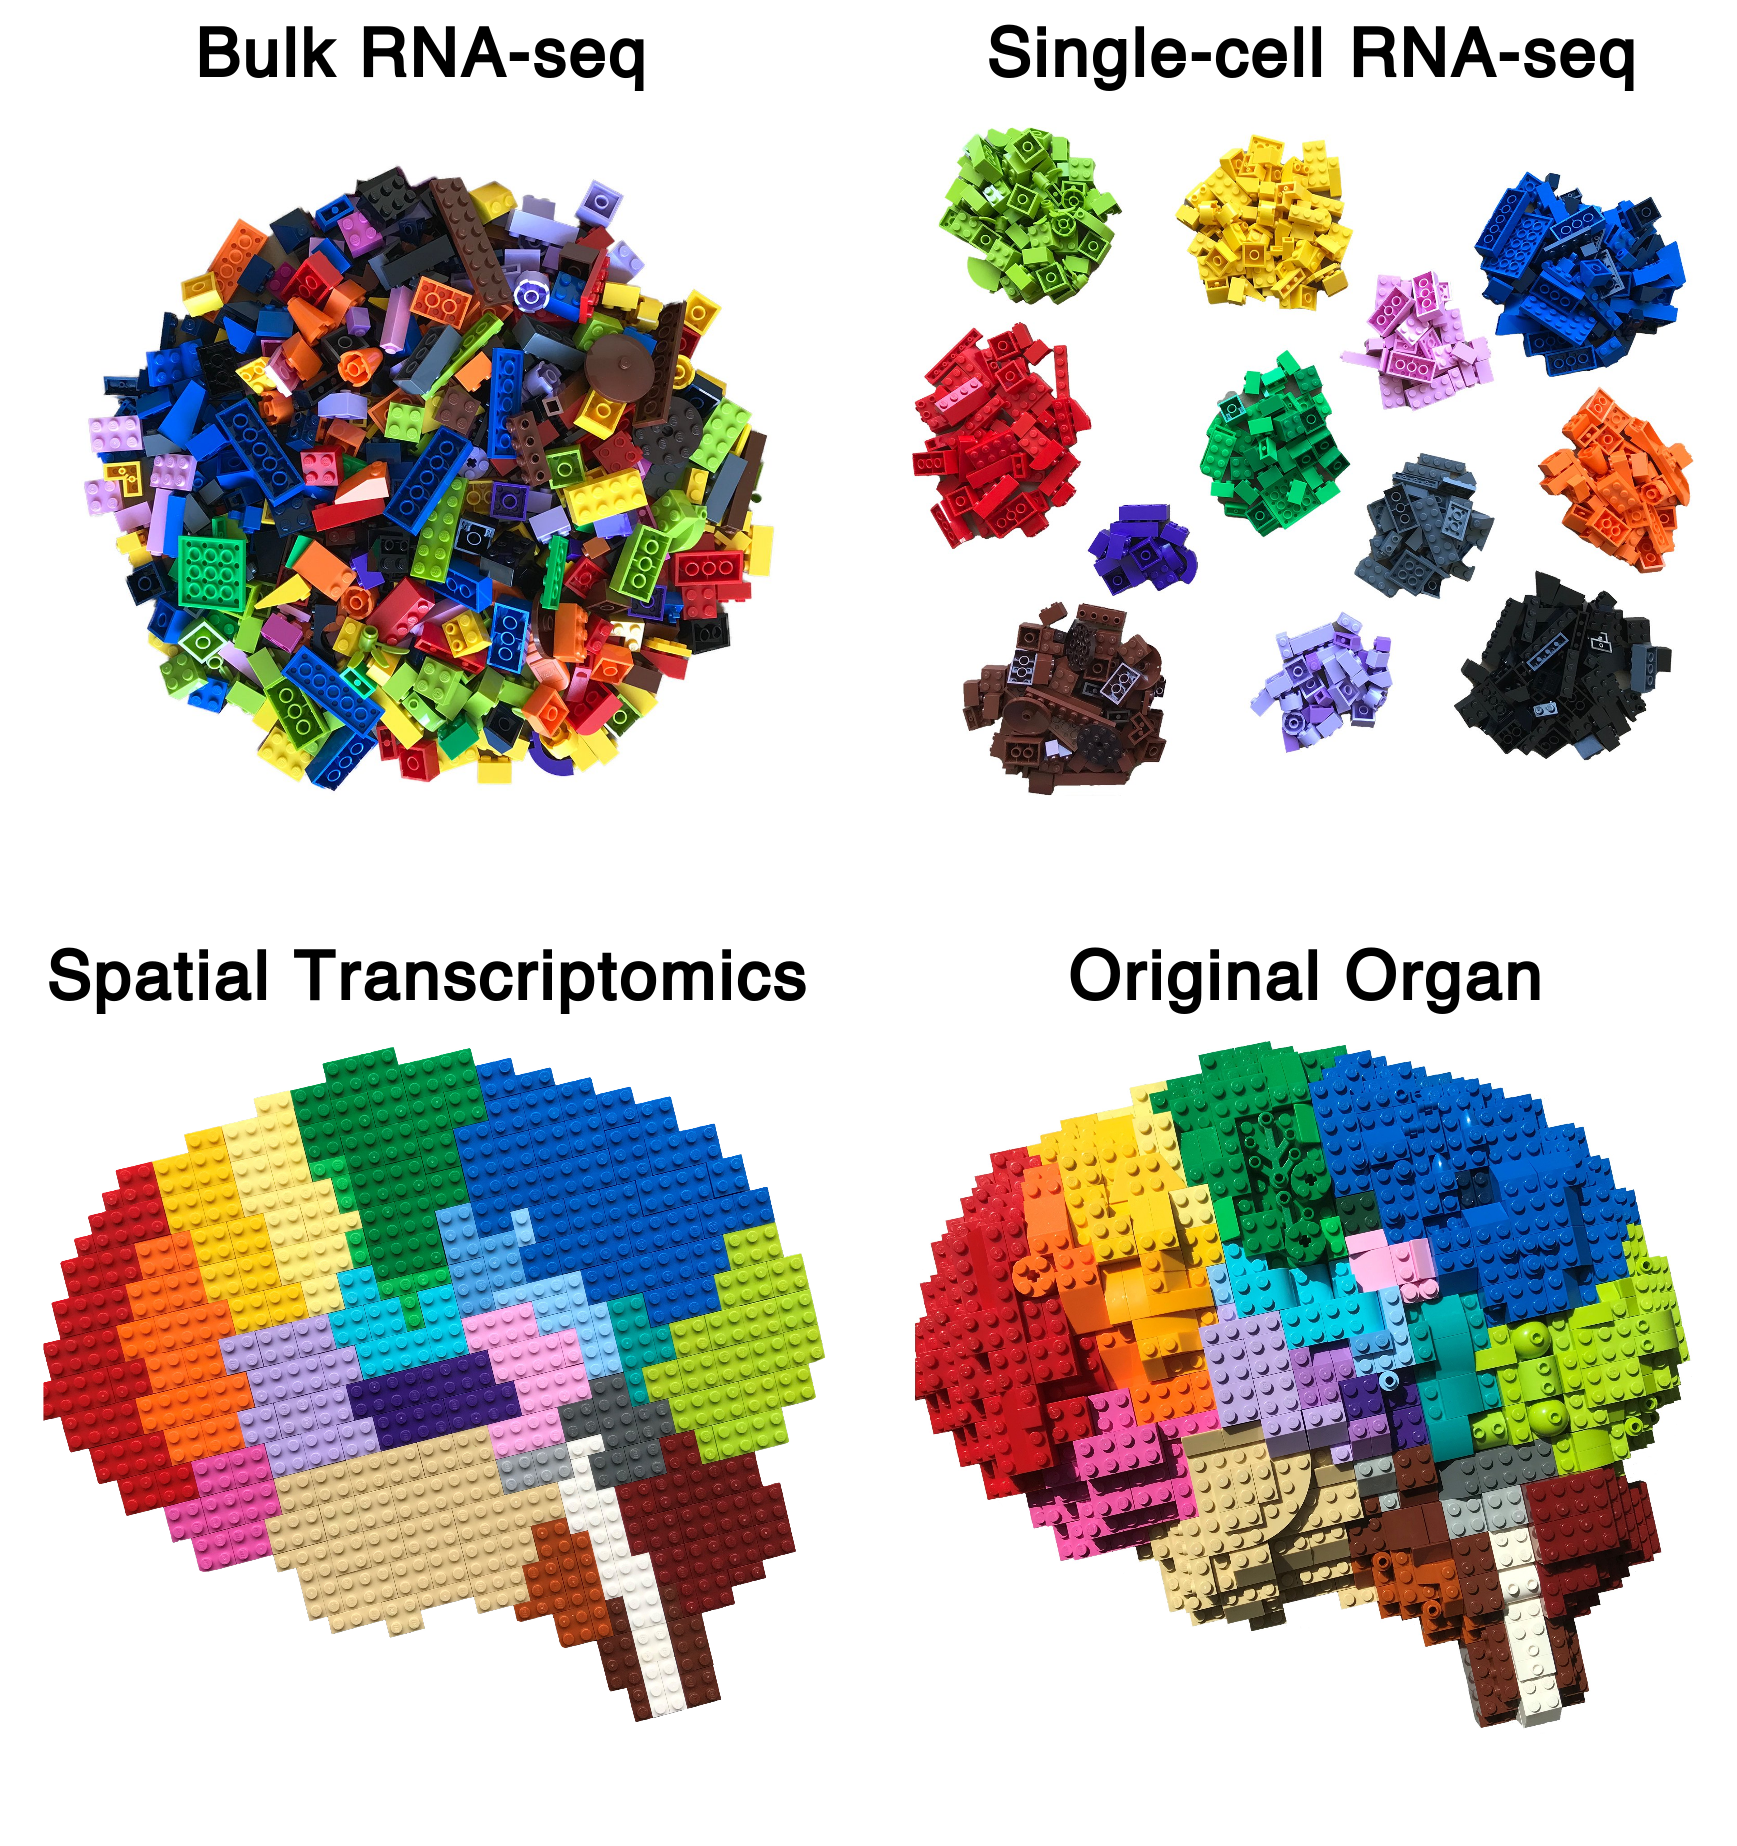
\includegraphics[width=250pt]{img/transcriptomics_experiment_types.png}
\caption[Visualization of Transcriptome Profiling Techniques]{Visualization of the transcriptome profiling techniques bulk RNA-seq, single-cell RNA-seq, and spatial transcriptomics, as well as the original tissue donor organ using toy bricks. Each brick represents one cell, and color coding depicts cells with similar expression patterns and thus similar phenotype.}
\floatfoot{Image credit: Bo Xia (\url{https://twitter.com/BoXia7})}
\label{fig:transcriptomics-techniques}
\end{figure}

A specific variant of HTS -- sequencing by synthesis -- was originally developed by the company Solexa, and later bought by Illumina. Also referred to as Illumina sequencing, it is currently the most commonly used sequencing technology with an estimated worldwide instrument market share of 80\% \cite{illumina-market-share}. All studies included in this thesis make use of data generated using Illumina RNA-seq, and the technique is described in detail in Section~\ref{subsec:sequencing-by-synthesis}.

While Illumina sequencing is currently the most commonly used technology, in the last few years third-generation sequencing or long-read sequencing has gained traction. These technologies, most prominently developed by the companies Oxford Nanopore and Pacific Biosciences, enable read lengths of tens of thousands of bases (Pacific Biosciences) to more than one million bases (Oxford Nanopore). These characteristics open up new opportunities to fill the gaps in reference genomes (see Section~\ref{subsec:reference-genome}), improve SV detection~\cite{Mahmoud:2019}, and variant calling in traditionally difficult to handle genome regions, as demonstrated in the precisionFDA Truth Challenge V2~\cite{Olsen:2020}. 


\subsection{Transcriptome Profiling}
\label{subsec:rnaseq}

Different techniques are available for probing the cancer transcriptome. Expression microarrays became available in the early 2000s and could be used to measure the expression of known genes and isoforms. Around 2010, high-throughput short-read sequencing (RNA-seq) started to evolve~\cite{Wang:2009} and has since effectively replaced microarrays as the principal method for transcriptome profiling. Unlike expression microarrays, RNA-seq is not restricted to known sequences and provides single base-pair resolution. The three most important steps in RNA-seq evolution are visualized in Figure~\ref{fig:transcriptomics-techniques}. Bulk RNA-seq was the first available technique and provides an average readout across the input material. Single-cell RNA-seq became available in the early 2010s and gives a readout on the level of individual cells. Spatial transcriptomics was developed in 2016 and enhances single-cell RNA-seq by enabling spatial resolution of mRNAs in individual tissue sections~\cite{Stahl:2016}. The focus of this thesis is bulk RNA-seq, which will be referred to as RNA-seq from here on.

In recent years sequencing has been making inroads into the clinic and it is being used to stratify patients into relevant clinical subtypes, identify treatment-predictive or prognostic genomic aberrations, and to track minimal residual disease. In many modalities the focus has been on introducing DNA-based sequencing (DNA-seq) into the clinic, mostly in order to determine genomic driver alterations. RNA sequencing has received less focus outside of the research community, although some clinical applications in mendelian diseases~\cite{Gonorazky:2019, Murdock:2020, Lee:2020}, myeloproliferative neoplasms~\cite{Schischlik:2019}, childhood cancers~\cite{Wong:2020} and others have emerged. In many cases RNA-seq accompanies DNA-seq in multi-omics approaches~\cite{Roychowdhury:2011}, and is typically used for subtyping and gene expression signatures. However, the capabilities of RNA-seq beyond this use case are now being recognized, as evident from recent reviews that have highlighted the growing importance and capabilities of RNA-seq, both from a technical and clinical view~\cite{Byron:2016, CieslikChinnaiyan:2017, Stark:2019, Marco-Puche:2019}.

RNA-seq offers many advantages over previous methods. It has a greater dynamic range and reproducibility, and can detect \textit{de novo} transcripts such as fusion genes in addition to quantifying known transcripts~\cite{Wang:2009}. In addition to isoform and gene expression it offers single-base resolution, which unlocks a range of applications, for example the possibility to detect sequence variants~\cite{Piskol:2013, Horvath:2013, Radenbaugh:2014, Wilkerson:2014, Sheng:2016, Guo:2017, Siegel:2018, Neums:2018}, coarse copy-number aberrations \cite{Patel:2014-RNA-CNA, Crowley:2015-RNA-CNA, Talevich:2018-cnvkitrna, Flensburg:2020}, and structural variants~\cite{Ma:2018-Squid, Cmero:2020}.

Through its sweet-spot between the genome and the proteome, transcriptome profiling using RNA-seq may be a powerful first-line clinical diagnostic tool. By enabling profiling of expression and genomic alterations simultaneously and within an actionable timeframe from surgery, a variety of gene expression signatures, for example for treatment response prediction, can be applied and drug susceptibility and resistance mutations can be evaluated.


\section{Bioinformatics}
\label{sec:bioinformatics}

While computational methods have been used in biochemistry since the 1960s, for example through the work of Margaret Dayhoff~\cite{EckDayhoff:1966}, the initial sequencing of the human genome and the advent of high-throughput molecular techniques such as HTS have transformed biology into a data-driven subject that requires computational knowledge. The term bioinformatics was originally coined in the 1970s by Paulien Hogeweg and Ben Hesper to describe ``the study of informatic processes in biotic systems''~\cite{Hogeweg:2011}. Since then the term has evolved to describe a vibrant interdisciplinary field that develops, curates, and applies computational methods to transform data into biological and clinical insights. Bioinformatics encompasses a wide range of subject areas, including structural bioinformatics and proteomics, HTS, sequence analysis, and biological networks. An integral part of the field's culture has been the embrace of open source software development and permissible licenses for code and, increasingly, data~\cite{Quackenbush:2003, Douglas:2011, Prlic:2012}. In spite of its importance for the life sciences, the field still struggles with acceptance in the academic and medical realm, including lack of funding for development and maintenance of even critical methods~\cite{Siepel:2019}, as well as lack of recognition and career options~\cite{bioinf-career, Lewis:2016, Dragon:2020}.

Bioinformatics is a crucial part of HTS, as the sequencing process transforms a traditionally wet-lab problem into a computational problem. Data processing is performed using computational pipelines or workflows, i.e. chains of different methods that work in concert to transform the data into the desired outcome or insight. To gain a better understanding of breast cancer and develop clinically meaningful diagnostic tools, the development of new computational methods and workflows is paramount.



%%%%%%%%%%%%%%%%%%%%%%%%%%%%%%%%%%%%%%%%%%%%%%%%%%%%%%
%
%                 Major Challenges
%
%%%%%%%%%%%%%%%%%%%%%%%%%%%%%%%%%%%%%%%%%%%%%%%%%%%%%%
\section{Major Challenges}
\label{sec:major-challenges}

Survival of breast cancer patients has improved in recent years, however many challenges remain. Screening programs have enabled the early detection of lesions and thus either the chance to remove them before potentially becoming malignant, or if already malignant, to prevent cancer from spreading. However, this has resulted in increased detection of \textit{in situ} lesions that would perhaps never develop into invasive breast cancer. Distinguishing harmless lesions from those that will become malignant is currently not reliably possible. As a consequence a significant fraction of women are likely cured by surgery and radiotherapy alone, or may only need comparably mild adjuvant therapy, but are being overtreated and thus suffer from unnecessary side effects, including long-term effects such as developing secondary cancer~\cite{Holland-Frei:9th}. In addition to its physical and psycho-social effects, overtreatment also poses a significant economic burden on healthcare systems \cite{Masood:2013} and the patients themselves. Much effort is being put into finding ways to downstage low-risk tumors to spare treatment, such as the TAILORx clinical trial and others~\cite{Gluz:2020}.
On the other end of the spectrum, patients who have lived disease-free for 15 years or more may still develop disease recurrence and ultimately succumb~\cite{Brenner:2002}. Distinguishing patients who will do well from those that will not is a major task for the future.
Current diagnostic tools are imperfect, and in addition to the cases mentioned above, they also falsely identify a small proportion of cases as low risk, when in fact they are high-risk and could perhaps benefit from more or different treatments. We partly address this challenge in study \III.

While treatment options have broadened in the last decades, resistance to drugs coupled with tumor heterogeneity continues to be a major challenge. External stimuli, such as treatments, provide selection pressure on the tumor and drive the evolution of resistant clones. Clones that harbor or develop a resistance mutation can thrive while competing clones succumb \cite{Gerlinger:2019}. Examples of clinically important resistance mutations are endocrine-resistance causing mutations in \textit{ESR1}~\cite{Toy:2013}, \textit{ERBB2}~\cite{Bose:2013, Nayar:2018}, genes of the \textit{FGF} and \textit{FGFR} families \cite{Mao:2020}, as well as activating \textit{ESR1} mutations and \textit{PTEN} loss of function mutations that lead to alpelisib resistance~\cite{Razavi:2020}. While resistance mutations are particularly prevalent in metastatic tumors~\cite{Robinson:2013, Nayar:2018}, they can already occur in treatment-naïve primary tumors~\cite{Dahlgren:2020}, as we also show in study \IV.

A major unmet need is effective treatments for the patient population with triple-negative tumors. While for other tumors targeted treatment options such as anti-hormonal or anti-HER2 therapies are available, TNBC tumors currently lack viable molecular targets and have poorer survival. In recent years several subtypes of TNBC have been identified~\cite{Lehmann:2011}, and alternative therapies such as PARP inhibitors and immune checkpoint inhibitors \cite{Vagia:2020} are in clinical trials and showing promise, possibly also in combination~\cite{Goncalves:2020}. Many of these tumors harbor germline or somatic \textit{BRCA1}/\textit{BRCA2} mutations, or exhibit ``BRCAness'', meaning they exhibit homologous repair deficiency but are not BRCA-muta\-ted~\cite{LordAshworth:2016}. These tumors can be detected using mutational and copy-number signatures such as HRDetect~\cite{Davies:2017}, and may likewise benefit from therapies such as PARP inhibitors.

The primary cause for breast cancer death is relapse of the disease in form of metastases. Detecting relapse is currently routinely being done using imaging techniques, either at regular checkup-intervals, or prompted by patient symptoms such as headache or bone pain. Since the early 2010s liquid biopsy approaches in form of circulating tumor cells (CTC) and circulating tumor DNA (ctDNA) have shown promise in tackling this problem~\cite{Olsson:2015, Garcia-Murillas:2015}. Both rely on the fact that tumors shed genetic material into bodily fluids such as blood where it can be detected in patient plasma from a simple blood draw. Prospective studies will be needed to bring these technologies into routine use for monitoring of minimum residual disease and treatment response.


%%%%%%%%%%%%%%%%%%%%%%%%%%%%%%%%%%%%%%%%%%%%%%%%%%%%%%
%
%                 Precision Medicine
%
%%%%%%%%%%%%%%%%%%%%%%%%%%%%%%%%%%%%%%%%%%%%%%%%%%%%%%
\section{Precision Medicine}
\label{sec:precision-medicine}

Precision medicine -- also called personalized medicine -- is an approach to tailor treatments to the specific genetic, environmental and lifestyle conditions of a patient. In cancer this means in particular determining and taking into account the genomic traits of the tumor and targeting its specific aberrations, as well as adjusting the therapy choices, doses, and durations depending on the clinical follow-up and predictive laboratory tests. The field is moving from designing drugs by tumor site to targeting specific genomic aberrations across different cancer types. For example a recent clinical trial of the HER tyrosine receptor kinase (TRK) inhibitor neratinib enrolled patients based on mutations in the \textit{ERBB2} and \textit{ERBB3} genes, independent of the tumor site~\cite{Hyman:2018-HER-trial}. Another trial evaluated the efficacy of the TRK inhibitor larotrectinib across cancers with TRK fusions~\cite{Drilon:2018}. A milestone for precision medicine occurred in the year 2017 when the drug pembrolizumab achieved approval by the FDA for treatment of solid tumors with microsatellite instability or DNA mismatch repair deficiency, independent of tumor type. This marked the first time a drug was approved based on genomic biomarkers alone instead of histopathology~\cite{Prasad:2018-biomarker}.

While precision medicine has many proponents, it is not without controversy~\cite{Prasad:2016}. Critics have noted that thus far few tangible success stories exist, despite high promises and expectations, and a great deal of money that has been spent in this area by funding agencies, nonprofit organizations, and corporations. Further, genome-driven oncology does not currently benefit the majority of U.S. patients~\cite{Marquart:2018}. Even for the ones it does benefit, the number of patients with measurable survival benefits varies~\cite{Prasad:2016}.

Besides matters of practical implementation and the arguments for and against precision medicine, it is important to keep its economic side in mind. Health care systems need to balance patient care with economic cost, which is a challenge in western societies due to rising cancer incidence and notoriously expensive cancer drugs~\cite{Prasad:2017-price, Tay-Teo:2019}. Genomics-guided diagnostics have the potential to drive down costs in the future by optimizing drug allocation and the ability to perform a multitude of computational tests and signatures based on data from a single laboratory test. Whether these hopes actually become reality needs to be determined by detailed economic studies, however preliminary studies indicate that sequencing benefits patients and is cost effective~\cite{Payne:2018, Marino:2018}.

As in most cases, the current reality about precision medicine lies between the extreme positions of its proponents and opponents. While the expectations on precision medicine were overly optimistic, particularly after the release of the first draft sequences of the human genome (see Section~\ref{subsec:reference-genome}) and the early days of HTS, the reality is that precision medicine is moving into the clinics. In certain modalities such as advanced non-small cell lung cancer (NSCLC), diagnostics technologies such as qPCR, dPCR, and targeted sequencing are routinely being used to test for the presence of biomarkers such as the \textit{EGFR} L858R mutation, which signals susceptibility to TKIs such as afatinib and crizotinib, and \textit{EGFR} T790M which confers resistance to these TKIs, but which can be overcome with other drugs such as osimertinib. While not all cancer patients currently benefit from genomic technologies and targeted treatments, these numbers will increase, as they already have between 2006 and 2016~\cite{Marquart:2018}. An example of precision medicine in real-life is the National Cancer Institute Molecular Analysis for Therapy Choice (NCI-MATCH) study (ClinicalTrials.gov identifier  \href{https://clinicaltrials.gov/ct2/show/NCT02465060}{NCT02465060})~\cite{Flaherty:2020} study, where patients are guided to therapies based on their genomic profiles across several tumor types.


%%%%%%%%%%%%%%%%%%%%%%%%%%%%%%%%%%%%%%%%%%%%%%%%%%%%%%
%
%                 SCAN-B
%
%%%%%%%%%%%%%%%%%%%%%%%%%%%%%%%%%%%%%%%%%%%%%%%%%%%%%%
\section{The Sweden Cancerome Analysis Network -- Breast (\scanb{}) Initiative}
\label{sec:scanb}

The Sweden Cancerome Analysis Network -- Breast (\scanb{}) Initiative (ClinicalTrials.gov identifier  \href{https://clinicaltrials.gov/ct2/show/NCT02306096}{NCT02306096}) is a precision medicine initiative started in 2009 by Prof. Åke Borg as a joint effort of researchers, physicians, nurses and other health-care specialists to improve diagnostics, treatment, survival, and quality of life for breast cancer patients. The initiative is described in detail in study \I and by Rydén \textit{et al} \cite{Ryden:2018-SCANB}. The \scanb{} study initially started enrolling patients in 2010 at seven participating hospitals in Malmö, Lund, Kristianstad, Helsingborg, Karlskrona, Halmstad, and Växjö, all located in the South Sweden healthcare region. Since then sites in Uppsala (2013) and Jönköping (2015) have joined the effort (Figure~\ref{fig:scanb-map}), and there is a standing open invitation to hospitals in the Nordics to join.

The goals of the initiative are threefold: to introduce gene expression and genomic tumor profiling into the clinical routine for breast cancer; to improve tumor classification, diagnosis, prognostication and prediction of treatment effects; and to make improvements accessible to patients through implementation within the healthcare system, clinical trials, and cooperation with the drug and biotechnology industry.

% SCAN-B map
\begin{figure}[t]
\centering
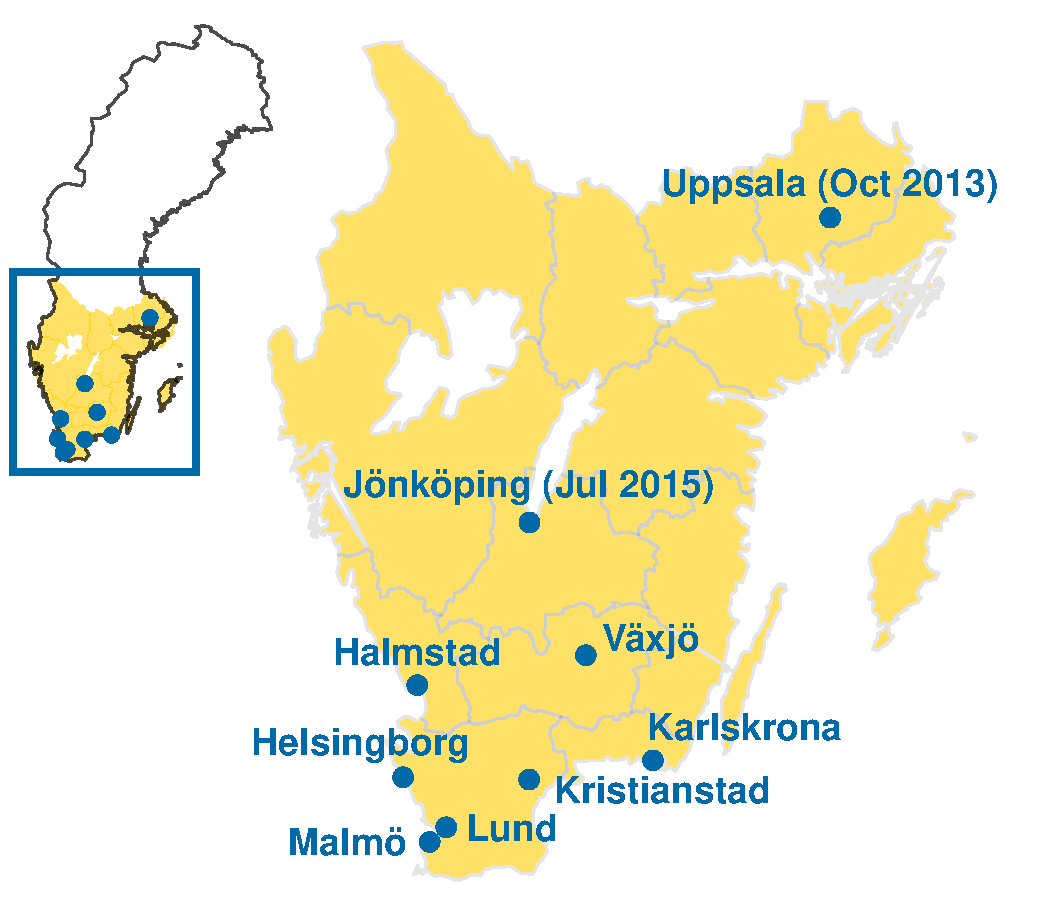
\includegraphics[width=220pt]{img/SCANB_map_v5.pdf}
\caption[Map of Sites Participating in SCAN-B]{Map of Sweden with the sites participating in the \scanb{} initiative marked: Malmö, Lund, Kristianstad, Helsingborg, Karlskrona, Halmstad, Växjö, Uppsala, and Jönköping.}
\label{fig:scanb-map}
\end{figure}

All patients with breast cancer at participating sites are eligible to enroll in \scanb{}, which started in August 2010 with the main \scanb{} study enrolling patients with primary breast cancer. In addition, since January 2019 patients with metastatic breast cancer are eligible to enroll in the \scanb{}-rec sub-study (ClinicalTrials.gov identifier  \href{https://clinicaltrials.gov/ct2/show/NCT03758976}{NCT03758976}). Each participating patient gives written informed consent, and donates a piece of their tumor as well as a pre-operative blood sample. After the surgery further blood samples are taken at defined follow-up time points. All samples are sent to the Division of Oncology at Lund University for central analysis and biobank storage. Currently the analysis process consists of performing mRNA sequencing (RNA-seq) of the tumor samples, typically within one week of surgery. This short time-span from surgery to data is critical for the eventual translation of biomarkers in a clinically-actionable manner.

Compared to earlier studies and patient cohorts, SCAN-B represents a significant advance. Patients have been treated with modern nationally standardized care regimens, such as anti-hormonal therapies and anti-HER2 therapies, and have been enrolled prospectively across a wide geography with nearly all new patients diagnosed being consented for SCAN-B. Older cohorts are often not representative since these treatments were not available at the time, or the cohorts are heterogeneous or not population-based, complicating comparisons with today's patients and thus seriously hindering their use in biomarker development. Its population-based nature and real-world conditions ensures that conclusions drawn from SCAN-B-based studies are representative and generalizable for the wider population. The importance of this was highlighted by Xie \textit{et al} \cite{Xie:2020} who analyzed 70 widely used public breast cancer gene expression datasets and found that they do not reflect the disease at a population level. Instead, high grade and ER- tumors are over-represented, potentially leading to biased conclusions. As of December 2020, more than 16,000 patients have consented to be part of \scanb{}, translating to approximately 85\% of eligible patients, and more than 13,500 RNA-seq libraries (including replicates) have been sequenced.

In addition to studies \I--\IV included in this thesis and many ongoing projects, the uses of the SCAN-B cohort thus far have covered research into many areas such as triple-negative \cite{Staaf:2019} and \textit{BRCA1}-abnormal tumors \cite{Glodzik:2020}, benchmarking of gene expression signatures \cite{Vallon-Christersson:2019}, investigation of gene fusions \cite{Persson:2017}, molecular subtyping \cite{Lundgren:2019, Sokilde:2019} and psychological resilience \cite{Axelsson:2018}, development of predictors of lymph-node metastasis \cite{Dihge:2019}, and comparisons of circulating tumor DNA (ctDNA) and circulating tumor cells (CTCs) for liquid biopsies \cite{Fornvik:2019}.


% ==================================
% CHAPTER: AIMS OF THE THESIS
% ==================================
\chapter{Aims}
\label{chap:aims}

\epigraph{``They're pretty high mountains,'' said Azhural, his voice now edged with doubt. ``Slopes go up, slopes go down,'' said M’bu gnomically. ``That's true,'' said Azhural. ``Like, on \textit{average}, it’s flat all the way.''}{--- \textsc{Terry Pratchett}\small\textnormal{, Moving Pictures}}


RNA-seq is a versatile yet underused technique for cancer diagnostics. The overarching aim of this thesis was to evaluate, explore, and improve the usability of RNA-seq as a clinical diagnostics tool within the \scanb{} project and breast cancer diagnostics.

The specific aims of the four studies included in this thesis were as follows: \\

\begin{tabularx}{\textwidth}{ rX }
\I   & To describe the \scanb{} study and its protocols and computational RNA-seq pipeline, provide an early evaluation of the enrolled patient cohort, evaluate the generated RNA-seq data by comparison of RNA-seq and expression microarrays performed on the same samples, and prototype variant calling. \\
\II  & To describe format validity problems in the widely-used RNA-seq alignment software packages TopHat and TopHat2 and develop a software tool to correct the problems. \\
\III & To assess variation within standard clinical histopathology, explore classification of clinically important biomarkers from RNA-seq-based gene expression profiles, and validate the classifications on overall patient survival in an independent cohort. \\
\IV  & To develop a computational pipeline for detection of somatic SNVs and indels from tumor-only RNA-seq data, and explore the mutational landscape of a large real-world primary breast cancer cohort in relation to patient overall survival.
\end{tabularx}


% ==================================
% CHAPTER: METHODS
% ==================================
\chapter{Methods}
\label{chap:methods}

\epigraph{Sometimes it's better to light a flamethrower than curse the darkness.}{--- \textsc{Terry Pratchett}\small\textnormal{, Men at Arms}}

\section{Patients, Samples, and Ethics}
\label{sec:patients}

All patients who contributed tumor material to the studies in this thesis were enrolled in the \scanb{} study, or the precursor study All Breast Cancer in Malmö (ABiM). As part of the enrollment process they were informed about the study by trained medical professionals, and patients provided written informed consent. Studies \I, \III, and \IV were approved by the Lund ethics review board and performed in accordance with the Declaration of Helsinki. Study \II did not include patient material or data and thus no ethics permissions were required.

% Cohort diagram from study III
\begin{figure}[t]
\centering
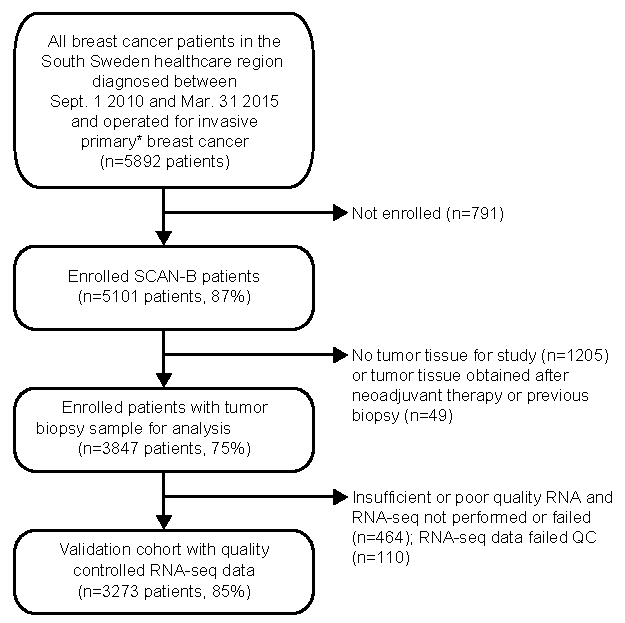
\includegraphics[width=240pt]{img/studyIII-cohort-diagram-original.pdf}
\caption[Patient Cohort Diagram for Study \III]{Patient cohort diagram for study \III. \textsuperscript{*} Non-metastatic primary unilateral breast cancer, which excluded patients with a diagnosis of synchronous (<3 months) contralateral invasive breast cancer.}
\floatfoot{Source: Adapted from Study \III, Supplementary Figure A1 (CC-BY 4.0)}
\label{fig:study3-patient-selection}
\end{figure}

The enrollment, biospecimen sampling, and analysis processes of the \scanb{} study are described in detail in study \I. Importantly, surgical tumor specimen are kept in RNAlater (Ambion) preservative after the routine pathology assessment, ensuring high quality RNA for later sequencing. Only remaining tumor material after the pathological assessment is included in SCAN-B, ensuring that SCAN-B enrollment is not a detriment to routine clinical care. ABiM samples were collected at surgery and stored fresh-frozen.

\begin{table}[h]
\centering
\caption[Patient Datasets and Experimental Setups]{Patient datasets and experimental setups used in studies \I, \III, and \IV.}
\label{tab:patients}
\begin{tabular}{ lllrrl }
\toprule
Source & Material       & Experimental Setup         & Patients & Samples & Study \\
\midrule
SCAN-B & Tumor          & RNA-seq / Microarray       &       49 &      49 & \I \\
SCAN-B & Tumor          & RNA-seq                    &    3,273 &   3,273 & \III \\
ABiM   & Tumor / Normal & RNA-seq / Targeted DNA-seq &      273 &     275 & \IV \\
SCAN-B & Tumor          & RNA-seq                    &    3,217 &   3,217 & \IV \\
\bottomrule
\end{tabular}
\end{table}

The patient cohorts and experimental setups used in this thesis are described in Table~\ref{tab:patients}. Study \I included 49 tumors that were analyzed using RNA-seq and expression microarrays. Study \III included 3,273 tumors, which were selected according to the flow diagram in Figure~\ref{fig:study3-patient-selection} to include all invasive, non-metastatic, unilateral breast tumors. For study \IV we used a cohort of 275 tumors from 273 patients (two patients with bilateral disease) assembled from the ABiM study, and re-used the cohort assembled for study \III. Applying additional quality checks reduced the number of patient tumors in the latter cohort to 3,217.


\section{DNA Microarrays}
\label{sec:microarrays}

DNA microarrays were first developed in the mid 1990s \cite{Shalon:1996} and were the dominant tool to measure RNA expression, SNPs, methylation, and other markers in the 2000s. They allowed the expression of large numbers of genes to be simultaneously measured for the first time. While RNA-seq has since become the preferred tool for expression profiling, microarrays are still widely used. Microarrays are chips with tens of thousands to hundreds of thousands of short oligonucleotide probes attached to a solid surface. The working principle is visualized in Figure~\ref{fig:microarray}. Each probe is complementary to a part of the target DNA molecule or ``feature'' to be measured. For gene expression profiling, the input mRNA is reverse-transcribed into cDNA and labelled with a fluorescent dye. The cDNA sample solution is then flooded over the chip, allowing the cDNA to hybridize to the probes, while unhybridized cDNA is washed away. Hybridization is quantified using a scanner that excites the labelled DNA using a laser and measures the resulting fluorescence. The resulting data needs to be analyzed while accounting for technical factors.

% Microarray probe hybridization
\begin{figure}[t]
\centering
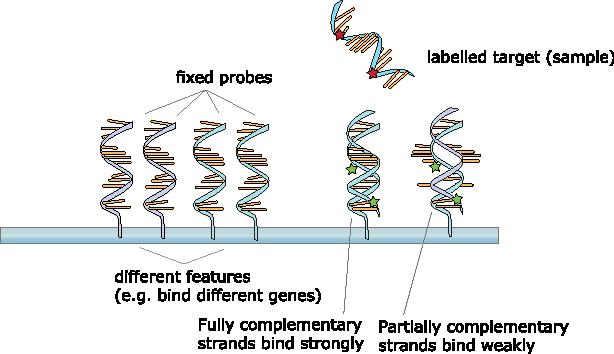
\includegraphics[width=300pt]{img/microarray_hybridization.pdf}
\caption[Microarray Working Principle]{Microarray working principle. Fluorescently labelled target sequences hybridize to complementary probes on the microarray surface. Probe-bound sequences produce a fluorescence signal when laser-excited (green stars), while unbound sequences are washed away and thus do not produce signals (red stars).}
\floatfoot{Source: \url{https://commons.wikimedia.org} (Public Domain)}
\label{fig:microarray}
\end{figure}

Microarrays have several limitations. First, they can only detect previously known sequences, since complementary probes need to be present on the chip for detection. In cancer, this means \textit{de novo} transcripts such as novel gene fusions, mutated transcripts, or unknown isoforms resulting from, for example, aberrant splicing cannot be detected. While microarrays can measure expression, they cannot resolve the more intricate features of the transcriptome such as RNA modifications, or sequence changes such as those caused by somatic mutations. Technical problems such as cross-hybridization and hybridization failure lead to high levels of background noise and missing values in the resulting data \cite{Wu:2005, Wei:2012}. High background noise and signal saturation limit the dynamic range so very low or very high expression cannot be accurately reflected. Due to variability of microarray platforms, comparison of microarray datasets from different platforms is inherently difficult and requires extensive normalization (techniques reviewed by Walsh \textit{et al} \cite{Walsh:2015}. Like many other high-throughput techniques, including RNA-seq, microarrays are prone to batch effects that influence interpretation and may have to be corrected \cite{Johnson:2007, Espin-Perez:2018}.

These technical problems pose challenges to the data analysis of microarray experiments. To compensate, microarrays typically contain control probes to estimate background noise. Using these, the estimated noise can be removed from all other measurements. Another common problem is missing values, since many downstream algorithms require complete data. This has led to the development of a variety of imputation methods to ``predict'' missing values from other samples, reviewed by Aittokallio \cite{Aittokallio:2009}. If a gene shows missing expression values in too many samples it is typically prudent to exclude it from further analysis, since incorrect imputation may lead to false conclusions.

In study \I we compared expression data resulting from the \scanb{} RNA-seq pipeline to Illumina Human HT12 v4 BeadChip microarrays covering 47,231 probes across the human transcriptome \cite{illumina-ht12-sheet}. While expression levels were comparable between the platforms, the comparison highlighted the superiority of RNA-seq compared to microarrays in terms of dynamic range and reproducibility. We also compared molecular subtyping based on three gene lists and found high concordance between the two technologies. However, this task highlighted another issue, in that probe annotations may be wrong or incomplete, but are required to map probes to their target mRNAs. For example in study \I we were able to match most but not all probes included in the Sørlie \cite{Sorlie:2003} and Hu \cite{Hu:2006} subtyping lists with our RNA-seq data.


\section{High-Throughput Sequencing}
\label{subsec:sequencing-by-synthesis}

High-throughput sequencing has revolutionized molecular biology. While third-generation technologies such as Pacific Biosciences single molecule real-time sequencing (SMRT) and Oxford Nanopore are gaining popularity, Illumina sequencing is by far the most commonly used \cite{Reuter:2015}. Depending on the setup it can be used for DNA sequencing (DNA-seq) or RNA-seq. Common DNA-seq experimental setups are WGS, WES, or targeted sequencing hybrid capture-based panels. The difference between these setups is which exact part of the genome is being sequenced. As part of study \IV, we used a custom hybrid-capture sequencing panel, while the remaining sequencing data in studies \I, \III, and \IV is based on whole mRNA RNA-seq.

% Illumina Sequencing
\begin{figure}[t!]
\centering

\includegraphics[width=\textwidth,trim=0 5cm 0 0,clip]{img/placeholder.png}
\caption[Illumina Sequencing Working Principle]{Illumina sequencing working principle using four distinct colors for the nucleotides \texttt{A}, \texttt{T}, \texttt{G}, \texttt{C}. \textbf{A.} The path from hybridization of template reads to the flow cell to cluster generation using bridge amplification. \textbf{B.} High-throughput sequencing using sequencing by synthesis with reversible terminators.}
\floatfoot{Source: Chaitankar \textit{et al} \cite{Chaitankar:2016}; reprinted with permission from Elsevier (panel C. not shown).}
\label{fig:illumina-seq}
\end{figure}

Illumina sequencing machines use a method based on sequencing by synthesis (SBS) and reversible terminators. The method was invented by Shankar Balasubramanian and David Klenerman, and first commercialized by the company Solexa, which Illumina acquired in 2007. A schematic of Illumina sequencing is shown in Figure~\ref{fig:illumina-seq}. The sequencing process is performed in a ``flow cell'' -- a compartment containing lanes through which reagents can flow in from one side, react with the surface, and are flushed out the other side. Depending on the sequencing machine model one or more flow cells can operate in parallel, with each flow cell containing multiple lanes. During sample preparation, sequencing adapters are ligated to the template cDNA molecules to be interrogated. These adapters are immobilized onto the flow cell surface using complementary bait oligonucleotides. Each immobilized template sequence is multiplied into a cluster of \textasciitilde1,000 sequences using bridge amplification (Figure~\ref{fig:illumina-seq}A). On the flow cell surface(s), many millions of clusters are generated which can then be sequenced simultaneously and in parallel. Depending on the setup, sequencing is performed in single-end or paired-end mode. In single-end mode, each molecule in a cluster is only sequenced from one end, resulting in a single read. In paired-end more, each molecule is sequenced from both ends, resulting in two reads. This provides additional information to subsequent \textit{in silico} analysis, as the expected distance between the paired reads, as well as their orientation is known. The sequencing process itself is performed in cycles, where each cycle starts by flooding the lanes with millions of deoxyribonucleotide triphosphates (dNTPs: \verb|A|, \verb|T|, \verb|G|, \verb|C|) that contain a reversible terminator that blocks polymerase activity (Figure~\ref{fig:illumina-seq}B). Each terminator is labelled with one of two or four (depending on the instrument) fluorophores that emit a different color when laser-excited. One dNTP is incorporated into each template strand on the flow cell. After that, two or four flow cell images are recorded, corresponding to the number of colors used and the terminators are removed so the next cycle can begin. Due to the presence of terminators, each cycle can only incorporate one base. The number of sequencing cycles is user-configurable, but is typically between 50 and 150 cycles, depending on the sequencing instrument. The per-cycle images are analyzed and converted into base calls by on-instrument software. In addition to the base calls themselves, Illumina sequencers assign a quality value to each call. This value is determined according to the Phred model shown in Equation~\ref{eq:phred} \cite{Ewing:1998a, Ewing:1998b}, where $P$ is the probability of calling a wrong base. A Phred score of 30 therefore equals a base call accuracy of 99.9\% (Table~\ref{tab:phred}). Base quality values are crucial for downstream analysis, and in a typical Illumina sequencing run the vast majority of bases have a Phred quality of ≥30.

\begin{equation} \label{eq:phred}
Q = -10\cdot\log_{10}(P)
\end{equation}

\begin{table}[t]
\centering
\caption[Phred Base Qualities]{Phred base qualities for defined base call accuracies.}
\label{tab:phred}
\begin{tabular}{ ccc }
\toprule
Phred Quality Score ($Q$) & Probability of Incorrect Base Call ($P$) & Base Call Accuracy \\
\midrule
10                      & 1 in 10                                & 90\% \\
20                      & 1 in 100                               & 99\% \\
30                      & 1 in 1,000                             & 99.9\% \\
40                      & 1 in 10,000                            & 99.99\% \\
50                      & 1 in 100,000                           & 99.999\% \\
\bottomrule
\end{tabular}
\floatfoot{Source: Illumina Technical Note: Quality Scores for Next-Generation Sequencing \cite{illumina-base-qual}.}
\end{table}

Multiple sample libraries can be sequencing in the same flow cell using multiplexing or pooling. During the library preparation DNA molecules are tagged using sample-specific barcode sequences. Multiple libraries are then pooled and sequenced concurrently. After sequencing the reads can be demultiplexed \textit{in silico} into sample-specific sequence files using their sample barcodes.

All sequencing data used in this thesis was generated using Illumina HiSeq 2000 and NextSeq 500 instruments. These instruments differ in their workings in that the HiSeq 2000 represents each of the nucleotides \verb|A|, \verb|C|, \verb|G|, and \verb|T| with a distinct fluorophore emitting a different color when laser-excited. The NextSeq uses a simplified system based on two colors where \verb|C| (red) or \verb|T| (green) are labelled with dedicated colors, \verb|A| is labelled with both colors, and \verb|G| is unlabelled. This system causes a reduction of the number of images that need to be taken during each sequencing cycle to two, down from four with the four-color system. While this simplified system has led to a decrease of sequencing price, it is more prone to over-calling \verb|G| bases, since a genuine base call cannot be distinguished from a situation where no signal is detected due to technical error, such as cluster degradation~\cite{two-color-chemistry}.


\section{RNA Sequencing}
\label{sec:rnaseq}

RNA sequencing using high-throughput short-read sequencing (RNA-seq) has emerged as the leading methodology for transcriptome profiling \cite{Wang:2009}. In recent years, it has effectively replaced microarrays as the principal method for transcriptome profiling since it offers many advantages over previous methods. RNA-seq has a greater dynamic range and reproducibility, detection of \textit{de novo} transcripts such as fusion genes in addition to quantifying known transcripts, as well single-base resolution. These capabilities enable a multitude of applications, such as the possibility to detect fusion genes and calling sequence variants \cite{Piskol:2013, Horvath:2013, Radenbaugh:2014, Wilkerson:2014, Guo:2017, Siegel:2018, Neums:2018}, coarse copy-number aberrations \cite{Patel:2014-RNA-CNA, Crowley:2015-RNA-CNA, Talevich:2018-cnvkitrna, Flensburg:2020}, and structural variants \cite{Ma:2018-Squid, Cmero:2020}, and the analysis of splicing and isoform switching \cite{Vitting-Seerup:2017}.

While the name suggests direct sequencing of RNA molecules, it is instead typically performed by sequencing cDNA resulting from RNA reverse-transcription. While direct Illumina short-read RNA sequencing is possible in principle, it has never matured and consequently is essentially unused \cite{Ozsolak:2009, Ozsolak:2011}. More recent sequencing technologies such as nanopore sequencing have been used to directly sequence RNA \cite{Geralde:2018, Soneson:2019, Hardwick:2019}, and even detect RNA modifications \cite{Leger:2019, Stephenson:2020}.

A general overview of the RNA-seq workflow from sample to result is depicted in Figure~\ref{fig:rnaseq-overview}. To prepare a sample for sequencing, input RNA has to be transformed into a sequencing library. All RNA-seq of SCAN-B samples included in this study were sequenced using a customized version of the stranded dUTP protocol \cite{Parkhomchuk:2009}. Selection of this protocol was made based the results of a comparison of stranded protocols from the literature \cite{Levin:2010} and an in-house comparison of the Parkhomchuk second strand dUTP approach, Illumina directional RNA ligation and the Epicentre ScriptSeq protocols. Newer libraries within the \scanb{} RNA-seq workflow have shifted to newer protocols and today use the off-the-shelf Illumina TruSeq protocol.

RNA-seq libraries can be prepared in a variety of ways. Two important properties are whether or not the library preserves information about which strand a transcript originated from (strand specificity), and whether single-end of paired-end sequencing is performed, i.e. whether a template molecule is only sequenced from one end, or both ends.

% High-level view of RNA-seq
\begin{figure}[t]
\centering
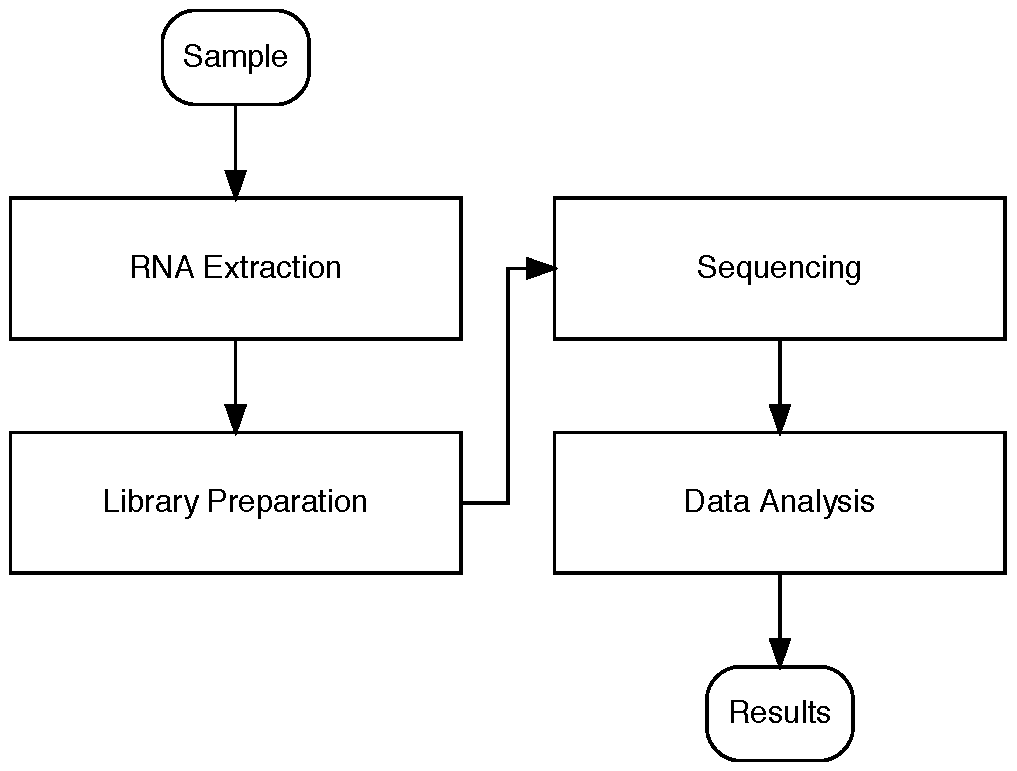
\includegraphics[width=230pt]{img/rnaseq-general-workflow.pdf}
\caption[High-Level View of the RNA-seq Workflow]{High-level view of the RNA-seq workflow.}
\label{fig:rnaseq-overview}
\end{figure}


\subsection{Library Preparation and Sequencing}

The RNA-seq data used in studies \I, \III, and \IV are based on libraries originating from a customized version of the strand-specific dUTP protocol by Parkhomchuk \textit{et al} \cite{Parkhomchuk:2009}, that is described in detail in study \I. While RNA-seq library preparation protocols have many commonalities with DNA-seq protocols, specific steps are included to ensure preservation of RNA properties. Most importantly, care has to be taken to preserve strandedness.

% dUTP library flowchart
\begin{figure}[t]
\centering
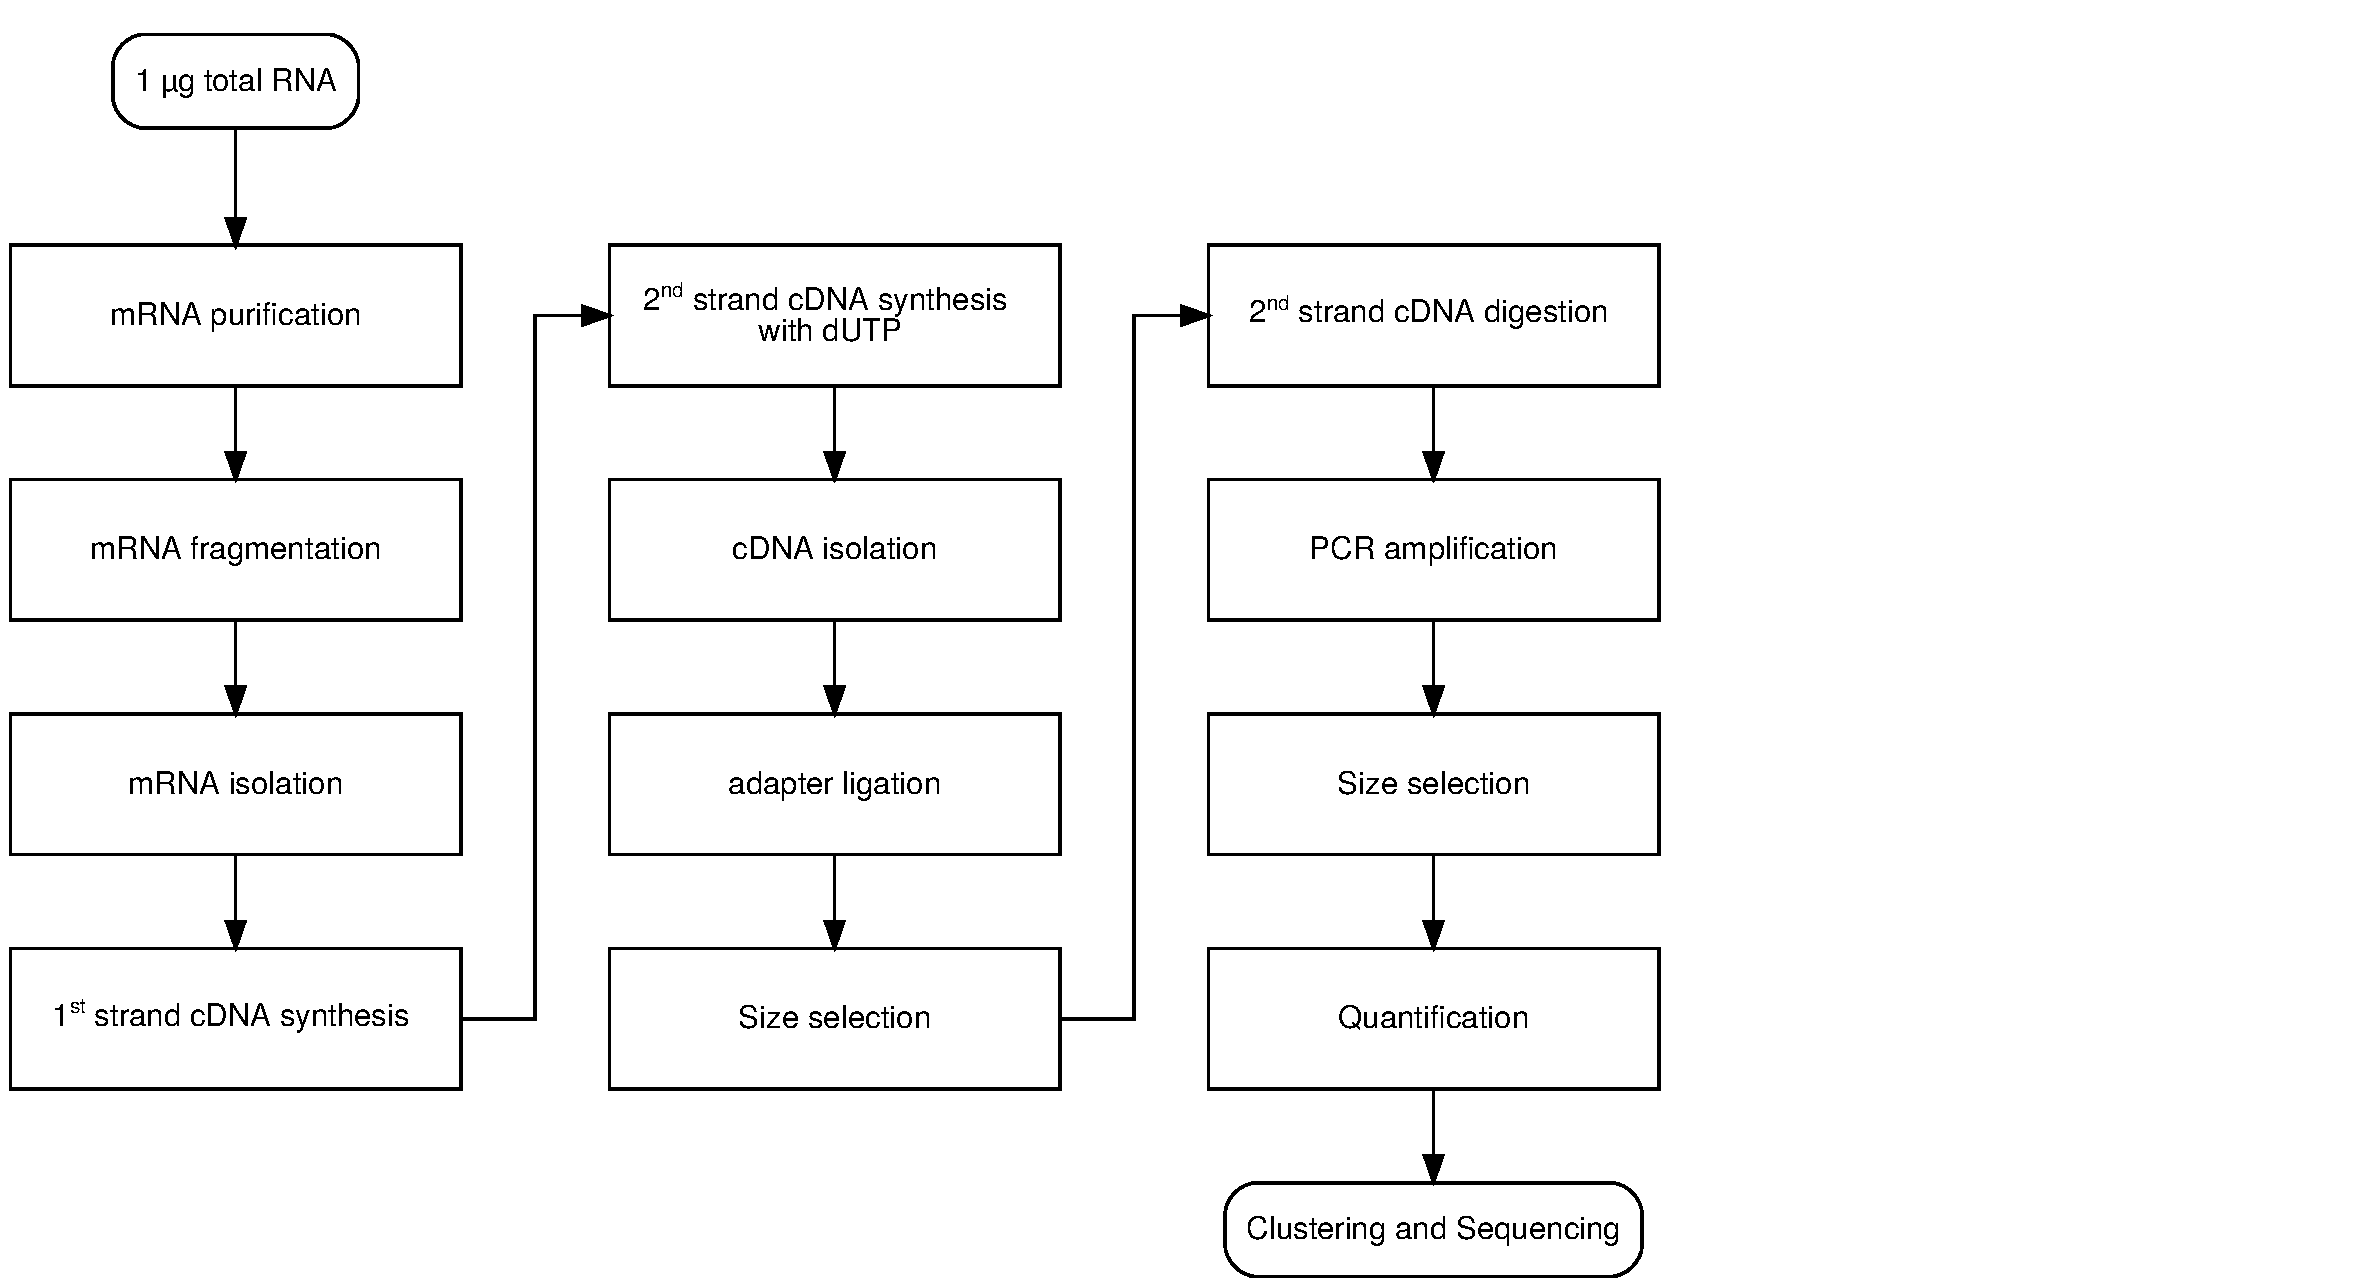
\includegraphics[width=320pt,trim=0 0 11cm 0,clip]{img/dutp-workflow.pdf}
\caption[Simplified dUTP Library Preparation Workflow]{Simplified workflow of the dUTP library preparation protocol.}
\label{fig:dutp}
\end{figure}

The customized dUTP protocol used for all \scanb{} samples included in the studies within this thesis is described in detail in study \I, and the steps are summarized in Figure~\ref{fig:dutp}. In brief, starting from 1$\mu{g}$ total RNA, mRNA is purified using poly-DT DynaBeads (Thermo Fisher Scientific), and subjected to Zinc-mediated fragmentation (Ambion). The resulting approximately 240bp fragments are isolated using Zymo spin columns (Zymo Research). Using the fragmented mRNA as input, first-strand cDNA synthesis is performed by adding random hexamer primers, reverse transcriptase, and dNTPs. Following cleanup of excess reagents, second-strand synthesis is initiated by adding polymerase and dNTPs with dUTP instead of dTTP. Resulting double-stranded cDNA is isolated using Zymo spin columns (Zymo Research), followed by 5'/3' end-repair and ligation of Illumina TruSeq sequencing adapters (Illumina), including sample barcodes. Size-selection is then performed to remove excess free adapters. To preserve strandedness, the dUTP-containing second cDNA strand is digested using uracil-DNA glycolase (UDG).

An important parameter in a sequencing setup is the average depth of coverage or number of reads to target for each samples. In a DNA-seq experiment, sequencing reads are distributed approximately uniformly along the targeted area of genome. An example target depth is 30X, meaning on average each targeted base is covered by 30 reads. Deviations from the uniform coverage assumption occur due to biases during library preparation and sequencing, for example caused by GC-rich regions \cite{Benjamini:2012, Ross:2013}. RNA-seq differs from DNA-seq in that reads are distributed approximately proportional to their expression level in the input sample, meaning that the average sequencing depth across an RNA-seq dataset is not a useful metric. Instead, the total number of sequencing reads is used to express how deep one has sequenced.

% HiSeq 2000: 2 flowcells with 8 lanes each, 16 samples multiplexes
% NextSeq 500: 1 flowcell with 4 lanes; automatic distribution across all lanes, first 16 then 24 samples multiplexed
The product of the library preparation process is a library of adapter-ligated double-stranded cDNA that is ready to be loaded onto a sequencer and multiple libraries are pooled. Within \scanb{}, on the HiSeq 2000 instrument library pools were sequenced across two flow cells in two lanes per flow cell to insure against technical failures and to reduce technical bias. The newer NextSeq 500 instrument loads one flow cell containing 4 lanes, and the library pool is automatically sequenced across all lanes. All RNA-seq samples included in studies \I, \III, and \IV were prepared using the dUTP protocol, and sequenced in paired-end mode on Illumina HiSeq 2000 or NextSeq 500 sequencers with a sequencing target of approximately 30 million read-pairs per sample.


\subsection{Computational RNA-seq Analysis}

Data processing and analysis is a key step in the RNA-seq workflow. The \scanb{} RNA-seq processing pipeline that studies \I, \III, and \IV relied on is implemented within the BASE laboratory information management system \cite{Base:2002, Base:2009} through the extension package Reggie \cite{Reggie:2016}. The pipeline follows the general computational RNA-seq workflow outlined in Figure~\ref{fig:rnaseq-workflow}, and is described in detail in studies \I and \III, as well as by Häkkinen \textit{et al} \cite{Reggie:2016}. It will be summarized here, and discussed in more detail in the following sections.

% RNA-seq computational workflow
\begin{figure}[t]
\centering
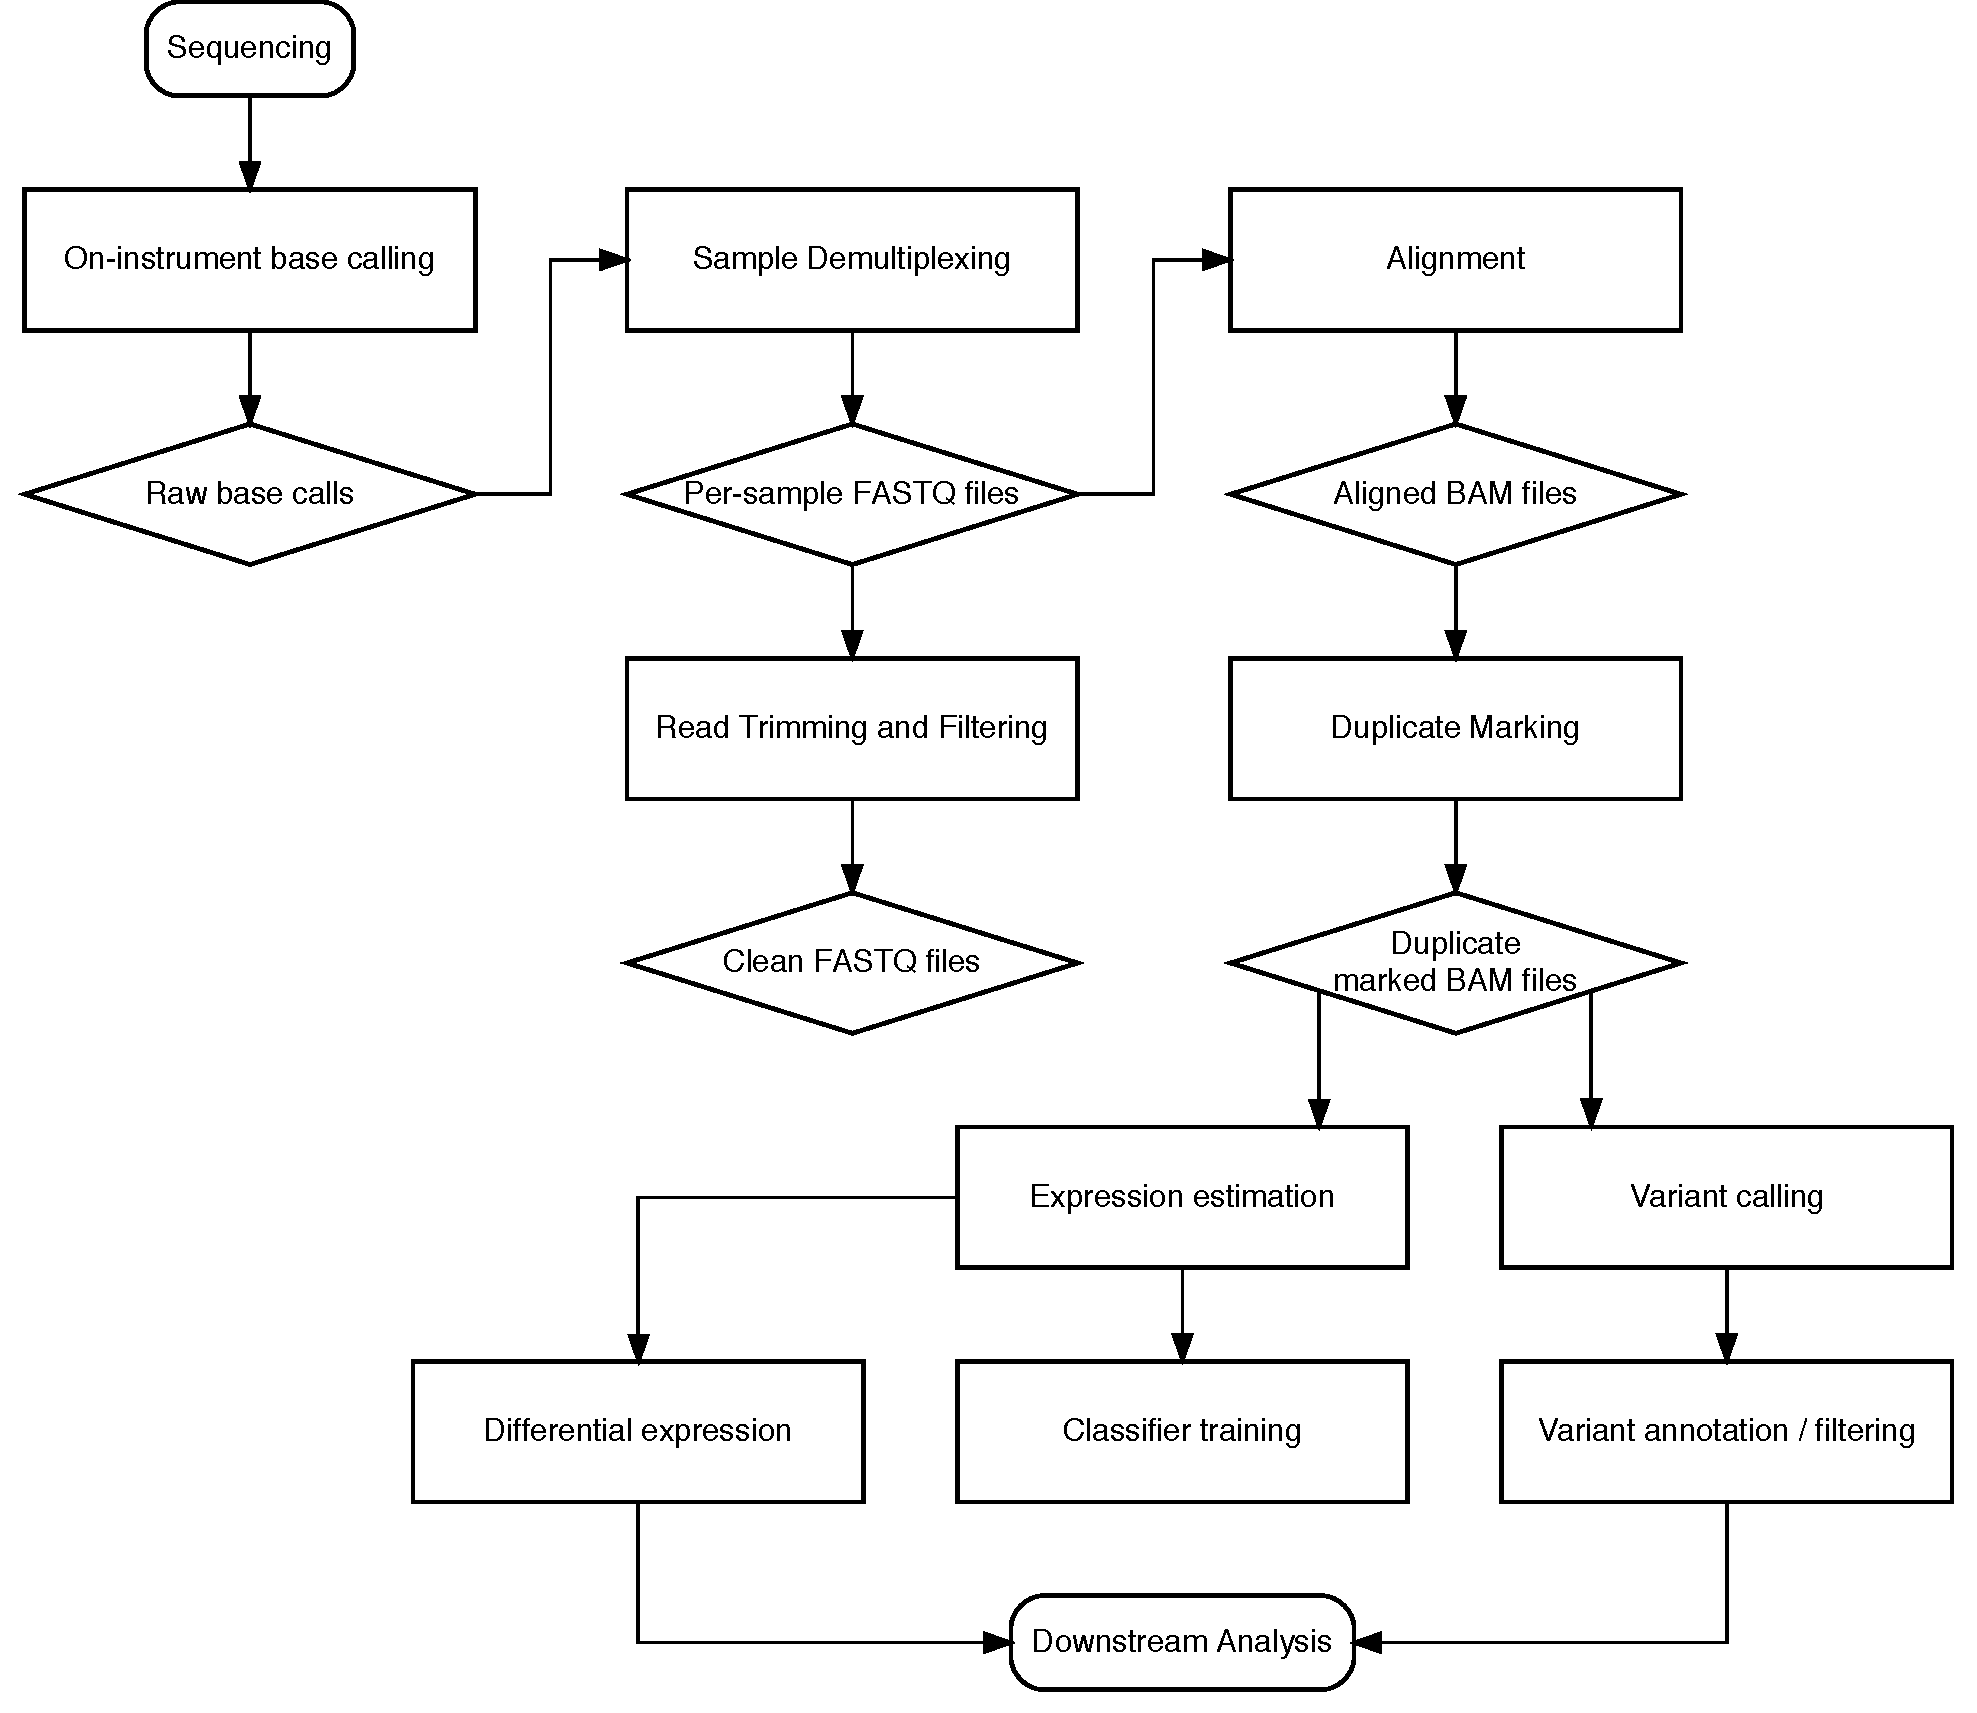
\includegraphics[width=\textwidth]{img/rnaseq-computational-workflow.pdf}
\caption[General Computational RNA-seq Workflow]{General computational RNA-seq workflow.}
\label{fig:rnaseq-workflow}
\end{figure}

In brief, the SCAN-B computational pipeline used in studies \I, \III, and \IV consisted of the following steps. Base-calling was performed using Illumina's on-instrument software. After sample demultiplexing, reads were trimmed to remove adapters and low quality 5'/3' bases using Trimmomatic \cite{Bolger:2014}. Reads that aligned to the PhiX phage genome, ribosomal DNA/RNA, or the UCSC RepeatMasker track \cite{repeatmasker} using Bowtie2 \cite{LangmeadSalzberg:2012} were removed. Bowtie 2 alignments were also used to estimate the fragment size distribution of the remaining reads. Using this information, reads were aligned to the GRCh37/hg19 (study \I) or the GRCh38/hg38 (studies \III and \IV) version of the human reference assembly and the UCSC knownGenes transcriptome model using TopHat2 \cite{Kim:2013-tophat2}. Unmapped reads were corrected using TopHat-Recondition as discussed in paper \II. Using the aligned reads, transcript expression was estimated using Cufflinks \cite{Trapnell:2010, Roberts:2011} and summed on the gene level.

More recently, \scanb{} samples are being processed with a pipeline that has been updated to use HISAT2 \cite{Kim:2019-hisat2} for alignment, and StringTie \cite{Pertea:2015} for expression estimation. These updates provide considerable improvements to both run-time and resource use. In addition, StringTie provides the ability to output read counts, which is the recommended input for differential expression profiling according to best practices \cite{Conesa:2016}.

The variant calling pipeline developed as part of study \IV was based on demultiplexed FASTQ files from the \scanb{} pipeline, but deviated from it from this point. Alignment was based on HISAT2 using a version of the GRCh38 reference assembly that included alternative sequences and decoys to optimize alignment and reduce artifactual variants caused by alignment problems. The pipeline was implemented within the bcbio-nextgen \cite{bcbio-nextgen} framework.

The individual steps involved in RNA-seq computational analysis are discussed in the following sections.


\subsubsection*{Demultiplexing and FASTQ Conversion}

Illumina sequencers convert fluorescence signals from read clusters into nucleotide base calls using Illumina's on-instrument CASAVA software. Base calls are stored in the Illumina-own BCL format. To convert BCL to the widely used FASTQ format, and to separate the pooled samples for further analysis, sequencing reads are demultiplexed into sample-specific FASTQ files. Two widely used software solutions for this task are the Illumina-own bcl2fastq and IlluminaBasecallsToFastq from the Picard suite \cite{picard}, which is used to demultiplex \scanb{} sequencing runs.


\subsubsection*{Read Trimming and Filtering}

Raw sequencing reads may be very short, contain adapter sequences, and/or low quality 5' and 3' bases, all of which may complicate subsequent analysis and in particular read alignment. Adapter contamination occurs when the cDNA template being sequenced is shorter than the requested read length and thus sequencing continues into the adapter. Low quality bases occur, for example, at the 5' ends due quality model calibration, and at the 3' end due to imperfect sequencing. Each cluster on the flow cell consists of \textasciitilde1,000 individual cDNA templates. After many sequencing cycles, synthesizing the individual reads can get out of sync causing lower confidence base calling.

Many computational pipelines, including \scanb{}, trim these potentially problematic read features to improve downstream analysis. Whether and how much trimming improves downstream analysis however, and which parameters are optimal, is often unclear and systematic evaluations of these questions are rare. An early study concluded that it is beneficial for germline variant detection, but not necessarily for expression profiling with modern alignment software such as TopHat2 \cite{DelFabbro:2013}. Similarly, a recent study concluded that trimming is not necessary for expression profiling, since modern aligners such as HISAT2 support soft-clipping \cite{Liao:2020}, which allows for low-quality read ends to remain in place in an alignment dataset, leaving it to downstream processing software to ignore or consider them. If trimming is performed, the choice of parameters that guide trimming aggressiveness have a substantial impact on analysis quality \cite{MacManes:2014}.

Sequencing datasets frequently contain unwanted reads. For example the PhiX lambda phage DNA is frequently spiked-in as a control, and RNA samples contain a large amount of ribosomal RNA (rRNA). Although RNA-seq library preparation protocols typically include rRNA depletion, or as within the \scanb{} protocol, selection of poly(A)-tailed RNA, these procedures are imperfect and rRNA may still be sequenced. Removing these sequences saves computational time and space, removes a potential of analysis errors, and improves expression estimation. Technically this is accomplished by aligning all reads against the unwanted sequences, and only selecting reads that do not align to these sequences for future analysis.


\subsubsection*{Alignment}

During read alignment, also called mapping, individual reads are placed into the correct position along a reference genome. For RNA-seq this is typically done with the help of a transcriptome annotation that provides information about splice junctions and transcript isoforms. Compared to aligners written for DNA, RNA-seq aligners are splicing-aware and can take this extra information into account during alignment. Aligners that fall into this category include TopHat \cite{Trapnell:2009}, TopHat2 \cite{Kim:2013-tophat2}, HISAT \cite{Kim:2015-hisat}, HISAT2 \cite{Kim:2019-hisat2}, and STAR \cite{Dobin:2013}. In studies \I and \III we used TopHat2 in combination with the post-processor TopHat-Recondition described in study \II to correct problems in unaligned reads. In study \IV we used HISAT2, the successor of TopHat2.


\subsubsection*{Duplicate Marking}

Duplicate reads most often occur as a product of PCR during the library preparation process (PCR duplicates) or due to the sequencer detecting the same template cluster multiple times (optical duplicates), but they can also occur naturally as true duplicates. Marking duplicate reads allows downstream analyses to ignore them, since in many cases they do not add additional information, but can bias analyses such as variant calling. Several software tools for duplicate marking exist \cite{Li:2009-samtools, Burriesci:2012, Tarasov:2015, Tischler:2014, Faust:2014} and virtually all of them follow the approach implemented by the MarkDuplicates tool from the Picard suite \cite{picard}. It works by comparing the 5' coordinates and sequences of single reads or read-pairs. Matching reads/read-pairs are ranked by the sum of their base qualities, and all but the highest scoring read/read-pair are flagged as duplicate. While the tools work similarly at the core, they differ in implementation, which influences performance and functionality. For example, biobambam supports steaming, meaning it can operate in Unix pipes, while Picard MarkDuplicates does not \cite{Tischler:2014}.

Whether or not marking duplicates in RNA-seq data is appropriate is unclear, but may depend on the specific use case.  The chance that reads with the same start/end coordinates arise from distinct molecules is typically higher in an RNA-seq experiment compared to WES/WGS due to lower library complexity. On the other hand, library preparation involving PCR results in many reads that originate from the same molecule. Parekh \textit{et al} \cite{Parekh:2016} found the impact of duplicate marking on RNA-seq differential expression in the best case improved metrics only mildly, and could otherwise even be detrimental. On the other hand, Quinn \textit{et al} \cite{Quinn:2013} found duplicate marking beneficial in RNA-seq SNP detection. Not marking duplicates in this case can severely overestimate variant allele frequencies (VAFs), potentially leading to false positive calls (see Section~\ref{subsubsec:variant-detection}). Thus, whether or not to mark duplicates is a judgement call that has to be made with taking the experimental setup, for example the number of PCR cycles, and the analysis endpoint in mind.

The need for duplicate marking can be avoided or reduced by using PCR-free library preparation protocols, or by using unique molecular identifiers (UMIs) \cite{Kivioja:2012}, where during library preparation each input molecule is tagged with an individual barcode. After sequencing, reads can then be regarded as duplicated if they share barcodes and map to the same genome coordinates \cite{Smith:2017, umis, fgbio}. This approach is common in single-cell RNA-seq \cite{Islam:2014} and HTS approaches for sensitive variant detection.

The standard \scanb{} computational pipeline as used in studies \I, \III, and \IV performs expression profiling as analysis endpoint and does implement duplicate marking, although the Cufflinks expression estimation software does not exclude duplicate reads from analysis. The variant calling pipeline developed in study \IV is distinct from the standard pipeline, but does mark duplicates as well, for the reasons outlined above.


\subsubsection*{Expression Profiling}

Expression estimation on the transcript and gene level is the most common use-case for RNA-seq. Traditionally, the input for this type of analysis are sequencing reads that have been aligned to a reference genome, although methods based on pseudo-alignment have become available since \cite{Bray:2016, Patro:2017}. With the help of a transcript annotation that describes introns and exons, the number of reads can be counted per transcript. Raw counts are biased by transcript length and number of reads per sample so counts need to be normalized to enable within-sample and between-sample comparison. Different methods for normalization are available, all with their own biases and drawbacks \cite{Dillies:2013, Conesa:2016, Li:2017, Evans:2018}. Starting from raw read counts, the measures reads/fragments per kilobase of exon model per million mapped reads (RPKM/FPKM, for single-end/paired-end data respectively) were introduced as a measure for expression that is within-sample normalized for library size and transcript length \cite{Mortazavi:2008}. This makes it difficult to compare RPKM/FPKM measurements between samples \cite{Wagner:2012}. A later measure is transcripts per million reads (TPM), which accounts for the same factors, but reverses the order of normalization operations to enable better comparability between samples. Contemporary methods for differential expression analysis largely require raw counts, since they account for transcript length and library size themselves \cite{Conesa:2016}.

In studies \I, \III, and \IV we used expression estimated in FPKM as generated by Cufflinks \cite{Trapnell:2010, Roberts:2011}. To reduce skewing of the data and ease fold-change calculations and comparisons we further transformed the values using $\log_2(FPKM+C)$, with $C=0.1$. The addition of a constant is needed to avoid zeros, since $\log_2(0)$ is undefined. 


\subsubsection*{Variant Calling}
\label{subsubsec:variant-detection}

Variant calling (detection) of SNVs and indels from HTS data is important to identify somatic cancer mutations. Since HTS has become available, dozens of methods (callers) have been developed (partly reviewed and/or benchmarked in \cite{Roberts:2013, Xu:2014, Alioto:2015, Cai:2016, Kroigard:2016, Sandmann:2017, Bian:2018, Xu:2018, Chen:2020-varcall}). An important distinction is whether a method has been developed for germline calling, somatic calling, or both. Somatic variant calling, particularly in cancer genomes, poses additional challenges due to aneuploidy and potential artifacts due to challenging read alignment. The gold standard for somatic variant detection is calling using data from matched tumor and normal samples from the same patient. This setup allows the caller to reliably differentiate between somatic and germline variants. While DNA-seq can in principle recover variants genome-wide, RNA-seq variant calling is limited to the expressed parts of the genome. Even if a variant is expressed it may be missed, due to transcriptional processes such as NMD removing the mutated transcripts from view before they can be captured for sequencing. On the other hand, RNA-seq provides exceptional sequence coverage in highly expressed genes, which may be used to detect low VAF variants that may be missed by DNA-seq.

A wide variety of somatic variant callers is available, with VarScan \cite{Koboldt:2012}, VarDict/VarDict-Java \cite{Lai:2016}, and MuTect2 \cite{Benjamin:2019} being among the most widely used. While variant calling from DNA is the most common setting and not all somatic variant callers have been tested or are recommended for RNA-seq, several approaches for RNA-seq mutation calling, mostly in combination with matched tumor and/or normal DNA, have been developed \cite{Piskol:2013, Horvath:2013, Radenbaugh:2014, Wilkerson:2014, Sheng:2016, Guo:2017, Siegel:2018, Neums:2018}. Combined variant calling of tumor RNA and tumor DNA makes it possible to discern true somatic mutations from transcriptomic effects such as RNA editing, while the use of normal DNA has already been discussed.

Often, reference datasets such as those generated by the Genome in a Bottle consortium are used for benchmarking and optimizing variant calling pipelines \cite{Zook:2016, Chapman:2020}. These are currently focused on DNA-seq and comparably well characterized tumor RNA-seq datasets are missing.

For detection of SNVs and indels we used VarScan \cite{Koboldt:2012} in study \I, while in study \IV we used VarDict-Java, a reimplementation of VarDict \cite{Lai:2016} in the Java language. We switched from VarScan to VarDict-Java based on its streamlined workflow that performs realignment around indels, does not require sequence pileups as input, and generates a wealth of sequence-based annotations, as well as internal benchmarks that were later affirmed by external benchmarks \cite{Sandmann:2017, Bian:2018, Quaglieri:2020}. MuTect2 \cite{Benjamin:2019} only became available during the course of study \IV, and has since been used for RNA-seq data \cite{Coudray:2018, Yizhak:2019}. Quaglieri \textit{et al} \cite{Quaglieri:2020} determined that 30--40 million read-pairs are necessary to detect the majority of known recurrent mutations in the tested acute myeloid leukemia TCGA samples, which matches the sequencing target of approximately 30 million read-pairs per sample used by \scanb{}.

% Error Sources
\vspace{1em}
\textit{Error Sources}

A major challenge in variant calling is the differentiation between true somatic variants and false positive calls due to technical artifacts or germline variants, particular when calling using tumor-only data. Technical artifacts can occur at different levels before, during, and after the sequencing process (reviewed in \cite{Salk:2018}). Before sequencing, prolonged time between surgery and sample preservation by flash-freezing or RNAlater may lead to DNA/RNA degradation. During library preparation, several processes may induce artifacts, most importantly PCR amplification of DNA leading to misincorporations and chimeras \cite{Brodin:2013, Kebschull:2015, PotapovOng:2017}. The sequencing process itself is imperfect and can lead to wrong base calls, particularly in challenging regions such as repeats, homopolymer stretches, and GC-rich regions \cite{Minoche:2011, Benjamini:2012, Ross:2013, Schirmer:2016}. Even after sequencing, alignment artifacts may lead to false positive variant calls.

% Annotation
\vspace{1em}
\textit{Annotation}

The wide range of error sources necessitates extensive filtering to remove false-positive calls. To enable better filtering and aid in downstream analysis, variant calls need to be annotated with additional information that allows them to be evaluated in the genomic and clinical context. Relevant information includes locational context, such as nearby genes or location in an intron or exon, population frequency through databases such as dbSNP \cite{Sherry:2001-dbSNP} and the Genome Aggregation Database (gnomAD) \cite{Karczewski:2020}. Clinical information, such as cancer driver status and whether presence of the variant signals susceptibility or resistance to drugs, for example through database such as the Catalogue of Somatic Mutations in Cancer \cite{Forbes:2015, Sondka:2018-COSMIC} or CIViC \cite{Griffith:2017}, is particularly important in cancer. An additional layer is the predicted functional impact which can be obtained from tools such as PolyPhen \cite{Adzhubei:2010}, SnpEff \cite{Cingolani:2012-SnpEff}, and the Ensembl Variant Effect Predictor (VEP) \cite{McLaren:2016}. In study \I we used ANNOVAR \cite{Wang:2010} for annotation, while in study \IV we used vcfanno \cite{Pedersen:2016} due to its speed and flexibility.

% Filtering
\vspace{1em}
\textit{Filtering}

Using variant annotations added by the variant caller and during the annotation process, variants can be filtered using various criteria. The exact settings may vary depending on the specifics of the downstream analysis. For tumor-only somatic variant calling, filtering germline variants is essential. To compensate for the lack of a matched normal sample this can be partly addressed using global germline variant databases such as dbSNP \cite{Sherry:2001-dbSNP} and gnomAD \cite{Karczewski:2020}, and national resources such SweGen \cite{Ameur:2017}. For filtering of technical artifacts a variety of variables are important, for example base quality, proximity to low complexity areas such as repeats or homopolymers, and GC content. Since valid and clinically important variants may be filtered out, variants may be ``rescued'' by evaluating their presence in databases such as COSMIC \cite{Forbes:2015} and CIViC \cite{Griffith:2017}. Even after filtering, manual refinement and curation of variant calls is often necessary to establish clinical relevance. This process is not currently standardized, however standard operating procedures have been proposed \cite{Barnell:2019, Danos:2019}.

Technical background noise makes it challenging to detect variants below 1\% VAF, although sequencing approaches exist that go below this \cite{Stahlberg:2016, Stasik:2018}. Competing technologies such as digital PCR (dPCR) allow detection of single or up to few specific variants as low as 0.001\% VAF using assay technologies such as IBSAFE/SAGAsafe (SAGA Diagnostics) \cite{Arildsen:2019, Fornvik:2019, Isaksson:2019, Pettersson:2020} with lower cost and faster turnaround time than HTS.


\subsubsection*{Quality Control and Sequencing Metrics}

High-throughput sequencing is a complicated process comprised of many individual steps, ranging from the initial nucleic acid extraction from a sample, over the preparation of sequencing libraries, to the sequencing process itself. Each step may induce errors and biases, which makes quality control at various points in the process a necessity \cite{Sheng:2017}.

Basic quality control can be performed after demultiplexing to check whether base- and read-level metrics conform to expectations. Important metrics include the number of reads per sample barcode, average base quality and read length, GC and unique kmer content, and sequencing adapter contamination. These metrics are partly generated by demultiplexing software such as IlluminaBasecallsToFastq from the Picard suite \cite{picard}, the popular software FastQC \cite{fastqc}, and others. If quality problems are detected at this stage, further analysis can be avoided and the library can be re-sequencing, or a new library can be prepared. More advanced metrics can be examined after sequence alignment and duplicate marking. Interesting metrics at this level include the percentage of uniquely aligned reads, the percentage of duplicated reads, average insert size, and for paired-end sequenced libraries the percentage of properly paired reads, defined as read-pairs with both reads aligned within the expected distance and orientation. A variety of software packages for QC at this stage exist, including RNA-SeQC and Qualimap \cite{DeLuca:2012, Okonechnikov:2016}. A comprehensive quality analysis of early \scanb{} RNA-seq datasets has been performed previously \cite{Brueffer:2013}.

An important confounding problem in RNA-seq are batch effects, where technical factors add variation and thus have systematic impact on the results. In other words, they describe a setting where variation between samples can be better explained by technical factors than by true biological variation. This is a problem in particular for quantitative analyses such as expression estimation. Several approaches have been developed for detecting and correcting batch effects in high-throughput experiments in general, and expression data in particular \cite{Johnson:2007, Leek:2012, Lauss:2013, Leek:2014, Zhang:2020}. Within \scanb{}, laboratory and sequencing processes have been optimized to minimize batch effects, and the \textit{swamp} R package \cite{Lauss:2013} is used to correlate expression data with a set of clinical variables, as well as technical variables such as dates of library preparation and sequencing. 


\section{DNA Sequencing}

DNA sequencing in various forms is the most commonly used form of sequencing. Although this study focuses on RNA-seq, we used DNA-seq to optimize properties of our RNA-seq analyses. In study \IV we used 275 samples from 273 patients that were sequenced using a custom targeted panel of 1,697 genes and 1,047 miRNAs (Agilent SureSelect) \cite{Winter:2016a}.

The computational analysis pipeline is very similar to that discussed for RNA-seq in Section~\ref{sec:rnaseq}, but simpler in many ways, and excludes expression-related analyses that are specific to RNA-seq. Sequence alignment does not need to account for a transcriptome model including splice sites, making the alignment process easier. While variant calling from DNA-seq data is not a solved problem and considerable variation between approaches still exists \cite{Hofmann:2017, Ellrott:2018, Shi:2018}, it is easier compared to RNA-seq calling, since the complexity of the transcriptome does not contribute to false positive calls.


\section{Molecular Subtype Inference}
\label{sec:subtyping}

Since the description of the intrinsic molecular subtypes Luminal A-like, Luminal B-like, HER2-enriched, Basal-like and Normal-like \cite{Perou:2000, Sorlie:2003}, multiple gene signatures have been developed for classifying tumors \cite{Sorlie:2003, Hu:2006, Parker:2009, Haibe-Kains:2012, Paquet:2015-AIMS}. The PAM50 method \cite{Parker:2009} has become the \textit{de facto} standard for classifying tumor expression profiles into intrinsic molecular subtypes. It was named after the Prediction Analysis of Microarrays (PAM) \cite{Tibshirani:2002} method that was used to determine the subtype centroids, and the list of 50 genes the signature is based on. More recent and refined subtyping schemes such as IntClust \cite{Ali:2014} comprising ten subtypes derived from gene expression and CNVs have not gained much traction yet.

Inference of molecular subtypes is performed using single sample predictors (SSPs), defined by Perou \textit{et al} as ``$\ldots$ any predictor where the algorithm and any parameter values are exclusively determined from a training set, and test cases are assessed independently'' \cite{Perou:2010}. Widespread clinical translation of subtyping SSPs has been hampered by several factors, summarized by Staaf and Ringnér \cite{StaafRingner:2015}. Notably, different methodologies were found to be only moderately concordant on a cohort level, although they stratified prognosis similar to one another. There was a lack of robustness on a single sample level, where subtype inferences with different SSPs often disagree \cite{Weigelt:2010-ssp, Mackay:2011}. The causes for this include inexact subtype definitions exemplified by the progression from the initially suggested classification gene list \cite{Sorlie:2001} to the now widely used PAM50 signature, to unclear descriptions of methodology, all taken together leading to reproducibility problems \cite{Weigelt:2010-ssp, Sorlie:2010, Weigelt:2010-reply, Mackay:2011}.

An additional problem is that previously developed SSPs, including PAM50, rely on normalization methods such as gene centering against a large heterogeneous set of samples for robust classification \cite{Lusa:2007, Sorlie:2010}. Centering scales the expression of each gene across samples in the dataset so that the mean or median expression is 0. This compensates for different expression scales caused by technical platforms different from that originally used to train the SSP, as well as batch effects between datasets. This step adds an implicit dependency on other samples and contradicts the definition of an SSP as given previously.

To improve the robustness of subtype classification, a variety of different approaches have been proposed \cite{Paquet:2015-AIMS, Franks:2018, Raj-Kumar:2019, Cascianelli:2020, Chen:2020-subtypes, Yu:2020}. Particularly the Absolute Intrinsic Molecular Subtypes (AIMS) approach suggested by Paquet and Hallett \cite{Paquet:2015-AIMS} garnered interest, as it promises true single sample prediction. During training, AIMS generates a number of binary rules in the form ``\verb|ESR1 < FOXC1|'' that capture the relative within-sample expression between two genes in a specific subtype, and thus obviating additional normalization.

We performed inference of molecular subtypes in studies \I, \III, and \IV. Study \I was still at an early stage in the \scanb{}, were subtyping had not yet been implemented on a \scanb{}-wide level. For this study we used PAM50 subtyping implemented in the \textit{genefu} R package \cite{genefu}. In time for studies \III and \IV we refined our subtyping procedure by following the approach by Parker \textit{et al} \cite{Parker:2009} using a \scanb{}-internal reference dataset that matches the original Parker \textit{et al} cohort in terms of clinical characteristics. Before subtyping tumors, gene expression of the PAM50 genes for each tumor was centered to the reference dataset in order to normalize it to the original training cohort.


\section{Histopathology}

Histopathology is the mainstay of current cancer diagnostics. In breast cancer, immunohistochemistry (IHC) is routinely used to determine the status of the biomarkers ER, PR, HER2, Ki67, and NHG. It works by staining tissue slides with protein-specific antibodies, and counting or estimating the percentage of stained cells in a representative section of the slide. Using a cutoff value, the percentage is categorized, typically into the ``low'' and ``high'' categories. Generally, this technique is prone to reproducibility problems, both from a technical and human perspective. On the technical side, dozens of factor can influence good IHC results, such as choice of antibody and method of staining \cite{MeyerholzBeck:2018}. On the human side, the same IHC staining may be interpreted differently by two pathologists, or even by the same pathologist at different times. Considerable effort has been spent to standardize IHC for routine breast cancer biomarkers in terms of antibodies, procedures, and interpretation. This has resulted in very high concordance for ER and PgR. While HER2 reproducibility is good with IHC alone, additional gene copy-number testing using \textit{in situ} methods such as FISH or SISH is recommended in borderline cases to verify \textit{ERBB2} amplification \cite{Rakha:2015}. Reproducibility for NHG is considerably lower, mostly owing to the existence of the intermediate category grade 2. Ki67 only recently entered the clinical guidelines, and standardization efforts are still ongoing \cite{Leung:2019}. While concordance is improving, it does not reach the high standards of ER, PgR, and HER2 yet.

One way to improve reproducibility is digital pathology, where the IHC slides are scanned and scoring is performed by machine learning based pattern recognition \cite{Rizzardi:2012, Mungle:2017, VanEycke:2017, Naik:2020}. However, image recognition only addresses the variation caused by the reader; the technical problem of staining variation remains. Other approaches have evaluated the possibility of using gene expression based to determine biomarker status \cite{Kun:2003, Gruvberger-Saal:2004, Roepman:2009, Bastani:2013, Wilson:2014, Viale:2014, Varga:2017}, however they are still not widely used. An important consideration for gene expression based approaches is that gene expression and protein expression are not always well correlated. Processes such as NMD can remove mRNA transcripts before translation, and epitranscriptomic modifications may impact translation rates. The mechanisms of mRNA and protein correlation have been reviewed by Buccitelli and Selbach \cite{BuccitelliSelbach:2020}.

In study \III we evaluated the concordance between stains and between readers by performing a multiple-stain, multiple-reader evaluation in a cohort of 405 breast tumors. We also proposed gene expression based approaches of determining the status of ER, PgR, HER2, Ki67, and NHG, and validated classifiers for all five biomarkers in a large population-based \scanb{} cohort.


\section{Machine Learning}
\label{sec:machine-learning}

Machine learning refers to the process of teaching a computer to perform a task based on prior learning. The field encompasses a wide range of techniques. In genomics, the two most commonly used approaches are supervised and unsupervised learning \cite{LibbrechtNoble:2015}. This nomenclature refers to whether the actual classes or ``labels'' of the input data are available to the algorithm (supervised) or not (unsupervised). Supervised methods such as Random Forests and Support Vector Machines are often used for sample classification, while unsupervised methods such as k-means and hierarchical clustering structure data solely using the intrinsic properties of the dataset and are thus well suited for exploratory analysis. Artificial neural networks with many layers (``deep learning'') can be either supervised or unsupervised, depending on how they are used \cite{Ching:2018}.

Hundreds of learning algorithms have been developed, complicating selection and evaluation. According to the ``no free lunch'' theorem \cite{Wolpert:1996}, there is no one algorithm that is clearly superior in all use cases, and an approach that works well in one problem domain may work poorly in a different one. In general it is unclear whether machine learning methods are generally superior to simpler statistical approaches such as logistic regression \cite{Lynam:2020}.

% https://twitter.com/TDataScience/status/1304799684054126599?s=20
% Model training methodology
\begin{figure}[t]
\centering
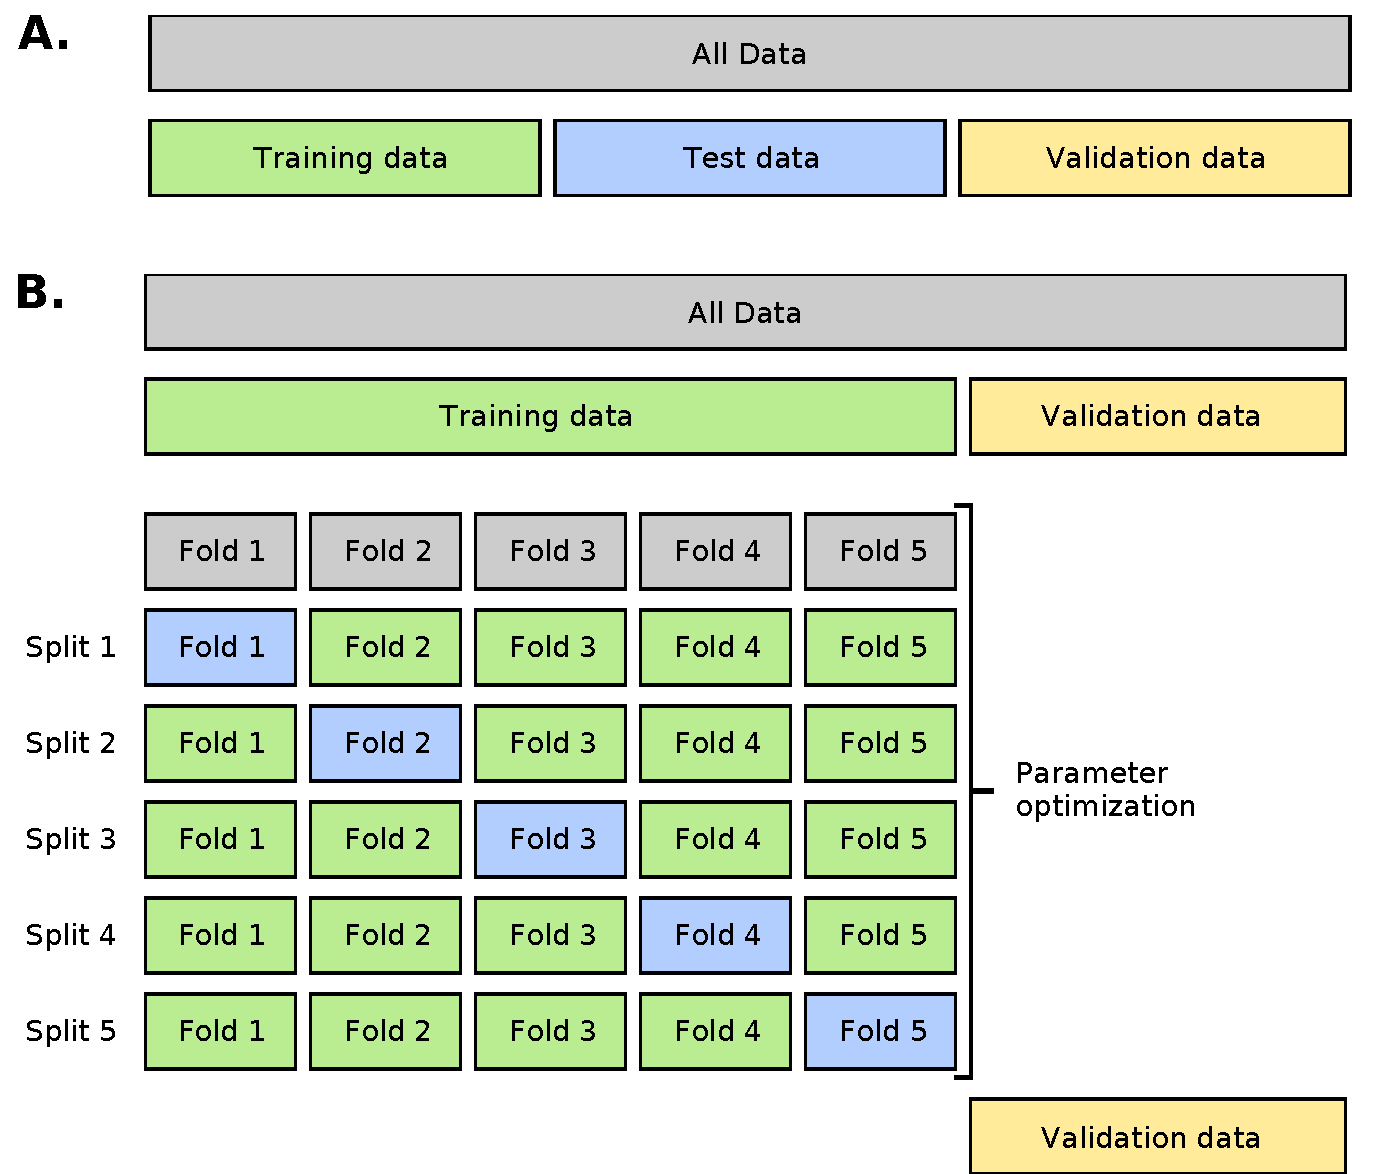
\includegraphics[width=\textwidth]{img/data_splitting.pdf}
\caption[Data Splitting for Model Training and Validation]{Data splitting for model training and validation. \textbf{A.} Standard data split into training, test, and validation datasets. \textbf{B.} Cross-validation data split into training and validation datasets.}
\label{fig:model-training}
\end{figure}

Machine learning in biology and particularly in genomics typically has to deal with the ``curse of dimensionality'', where the number of features (variables) is much larger than the number of observations (samples). Thus, a major consideration in supervised machine learning is bias due to overfitting which can reduce the generalizability of a model. Overfitting can be counteracted in multiple additive ways. The best but often most impractical way is increasing the number of samples. Generally, simpler models are less likely to suffer from overfitting than complex models. Ways to achieve simpler models are removing features or adding regularization which penalizes complex models. Splitting data appropriately for training and testing is another way to avoid overfitting. Data is typically split into three subsets: training, test, and validation\footnote{There are differences in the nomenclature for test and validation in the literature, causing the two terms to be used interchangeably.} (Figure~\ref{fig:model-training}A). A model is fitted in the training set and evaluated in the test set. Based on the evaluation the model features and parameters can be adapted before being evaluated again. This training loop can be repeated as many times as needed, although this may, again, contribute to overfitting. Alternatively, particularly when the available dataset is small, cross-validation can be used (Figure~\ref{fig:model-training}B). During cross-validation, the sample set $N$ is split into $M$ equal partitions. $M-1$ parts are used for training and the $M$\textsuperscript{th} part is used as a test set. The procedure is repeated until every partition has been used as test set.

Importantly, information leaks from the validation dataset to the model must be avoided. These can happen for example when testing a model against the validation dataset and adjusting the model based on the results. In this case the validation dataset loses its independence and further tests of the adjusted model are invalid, as the performance measures obtained from it would not be generalizable.

In studies \I, \III, and \IV we used a variety of unsupervised and supervised methods. Study \I and \IV used hierarchical clustering to group samples based on gene expression and pathway mutations. In study \III we used the supervised PAM method based on nearest shrunken centroids \cite{Tibshirani:2002} implemented in the \textit{caret} and \textit{pamr} R packages \cite{pamr, Kuhn:2008-caret} to develop classification models for the breast cancer biomarkers ER, PgR, HER2, Ki67, and NHG based on gene expression data. A centroid here is the mean expression value of all included genes. The method was initially developed for microarray-based transcription profiling and thus can handle highly dimensional data. It works by calculating a standardized centroid for each class in the training dataset by dividing the per-class centroids by the respective within-class standard deviation, and afterwards ``shrinking'' the per-class centroids towards the overall centroid by a user-configurable threshold parameter. The shrinkage step reduces the effect of noise and eliminates non-informative genes \cite{Tibshirani:2002}. To classify a new sample, the standardized centroid for this sample is calculated, and the distance to each per-class centroid is determined. The sample is then assigned the class with the shortest distance of its per-class centroid to the sample centroid. In our study we used repeated cross-validation to optimize the shrinkage parameter, train classification models, and estimate the variation across multiple different cross-validation splits. We validated the resulting classifiers in a large cohort of breast cancer samples. We strictly adhered to keeping the validation set independent and only used it to evaluate the final models.

While we developed RNA-seq variant filters in study \IV using a training and validation set, we did not aim to keep the validation set independent. Due to the complexity of the problem we instead explicitly used information from the validation set to improve the filters. As such the filters may be overfitted to \scanb{} data and not generalizable to other datasets.


\subsection{Classifier Performance Metrics}
\label{subsubsec:classifier-metrics}

% Confusion matrix
\begin{figure}[t]
\centering
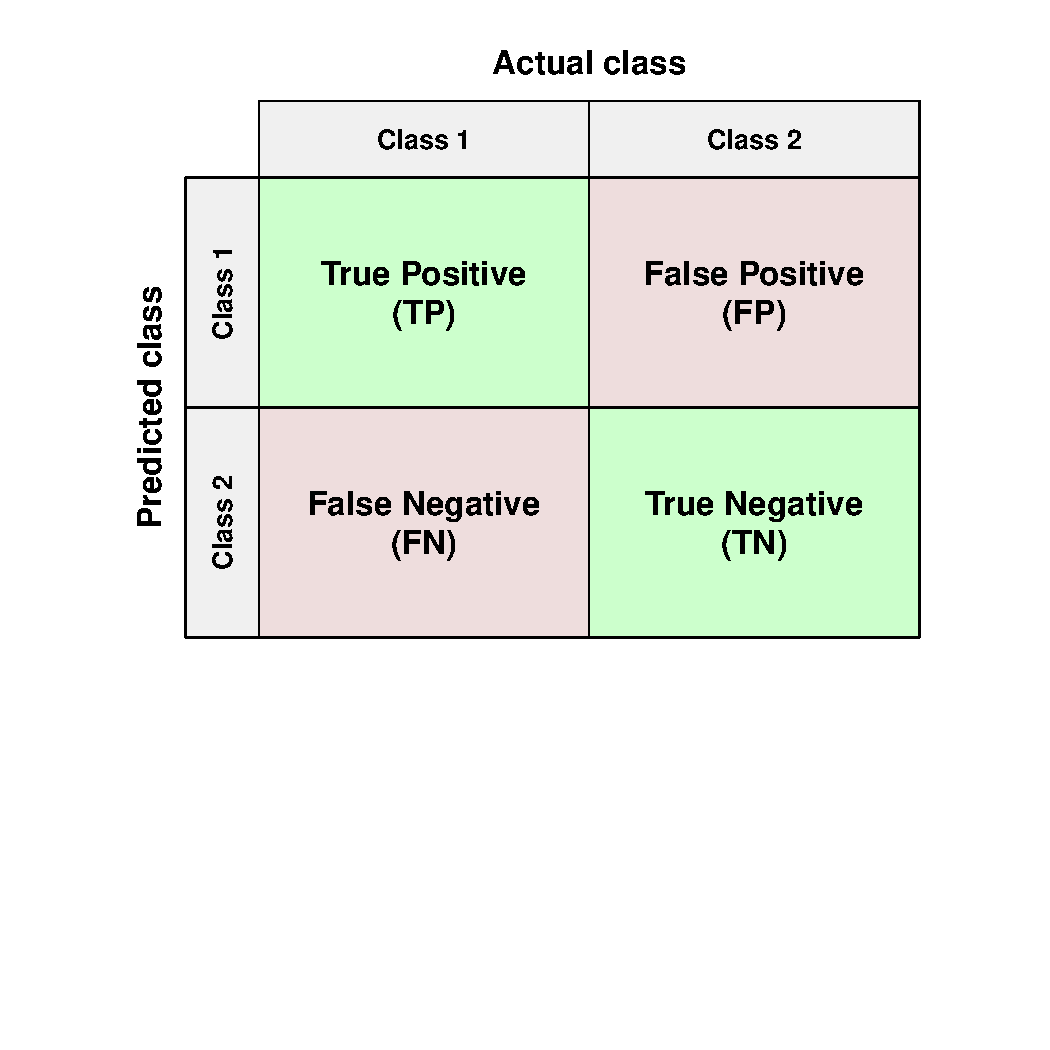
\includegraphics[width=270pt,trim=0 6cm 0 0.5cm,clip]{img/confusion-matrix.pdf}
\caption[General Confusion Matrix]{Confusion matrix for two-class problems, consisting of true positives (TP), true negatives (TN), false positives (FP), and false negatives (FN).}
\label{fig:confusion-matrix}
\end{figure}

The performance of a binary classification model can be expressed through a confusion matrix (Figure~\ref{fig:confusion-matrix}) which describes true positives (TP), true negatives (TN), false positives (FP, Type I errors), false negatives (FN, Type II errors). Based on these a variety of model performance metrics have been developed. Simple measures such as accuracy (Equation~\ref{eq:accuracy}) assess raw performance, but do not account for the fact that a classification model can ``guess'' right just by chance. More sophisticated measures such as Kappa (Equation~\ref{eq:kappa}) and Matthews Correlation Coefficient (MCC; Equation~\ref{eq:mcc}) take this chance effect into account. These metrics are commonly interpreted according to a scheme proposed by Viera and Garrett \cite{VieraGarrett:2005}, outlined in Table~\ref{tab:kappa-interpretation}, that adds intuition to the pure numbers.

A common way to visualize the performance of a classifier using different thresholds is plotting the receiver operating characteristic (ROC) curve using the metrics sensitivity and $1-$specificity. Other graphical methods that are thought to perform better than ROC for unbalanced datasets include precision/recall curves and MCC-F1 curves \cite{Cao:2020}. One can then select the threshold that maximizes the area under the curve (AUC).

Which metric to use for classifier evaluation during training includes the question which property of a classifier to prioritize. In study \III we used balanced accuracy (Equation~\ref{eq:balanced-accuracy}) \cite{Brodersen:2010} during training for this task, since it strikes a balance between sensitivity and specificity, and works well in unbalanced datasets. For performance evaluation in the validation dataset we used accuracy (Equation~\ref{eq:accuracy}), MCC (Equation~\ref{eq:mcc}), Kappa (Equation~\ref{eq:kappa}), and positive/negative predictive value (Equations~\ref{eq:ppv} and~\ref{eq:npv}).

\begin{table}[t]
\centering
\caption[Interpretation of the Kappa and MCC Statistics]{Common interpretation of the Kappa and MCC statistics according to Viera and Garrett.}
\floatfoot{Source: Viera and Garrett \cite{VieraGarrett:2005}}
\label{tab:kappa-interpretation}
\begin{tabular}{ ll }
\toprule
Kappa / MCC & Agreement \\
\midrule
$\leq0$     & Less than chance \\
 0.01--0.20 & Slight \\
 0.21--0.40 & Fair \\
 0.41--0.60 & Moderate \\
 0.61--0.80 & Substantial \\
 0.81--0.99 & Almost perfect \\
\bottomrule
\end{tabular}
\end{table}

% Summary
% http://www.john-uebersax.com/stat/agree.htm

Accuracy (ACC):
\begin{equation} \label{eq:accuracy}
ACC = \frac{TP + TN}{TP + TN + FP + FN}
\end{equation}

Balanced Accuracy (BACC):
\begin{equation} \label{eq:balanced-accuracy}
BACC = \frac{1}{2}(\frac{TP}{TP + FN} \cdot \frac{TN}{TN + FP})
\end{equation}

% http://www.john-uebersax.com/stat/kappa2.htm
% https://stats.stackexchange.com/questions/437369/fleiss-kappa-vs-cohen-kappa
Cohen and Fleiss' Kappa:
\begin{equation} \label{eq:kappa}
Kappa = \frac{(p_{o} - p_{c})}{(1 - p_{c})}
\end{equation}
where $p_{o}$ is the observed agreement, and $p_{c}$ is the chance agreement.

Matthew's Correlation Coefficient (MCC):
\begin{equation} \label{eq:mcc}
MCC = \frac{TP \cdot TN - FP \cdot FN}{\sqrt{(TP + FP)(TP + FN)(TN + FP)(TN + FN)}}
\end{equation}

Positive Predictive Value (PPV):
\begin{equation} \label{eq:ppv}
PPV = \frac{TP}{TP + FP}
\end{equation}

Negative Predictive Value (NPV):
\begin{equation} \label{eq:npv}
NPV = \frac{TN}{TN + FN}
\end{equation}



\section{Statistical Analysis}
\label{sec:statistical-analysis}

Statistical hypothesis testing deals with the question of whether or not a specific null hypothesis can be explained by the available data. They result in a probability (P-value) for obtaining the observed or more extreme results, for example the quantitative difference between two groups, if the null hypothesis were true. For better or worse, a P-value of P<0.05 is commonly interpreted as a difference being significant. Importantly, P-values only give the probability that an effect exists, but are not a measure of effect size. P-values are intricately linked with sample size in that large sample sizes can lead to small P-values even if the effect size is very small \cite{Lantz:2013}.

Based on their assumptions, statistical tests can be stratified into parametric and non-parametric tests. Parametric tests rely on the approximate normal distribution of the input data, while non-parametric tests do not. In studies \I, \III, and \IV we relied on 1-sided and 2-sided Fisher's exact tests for all hypothesis tests. Additionally we performed survival analyses in studies \III and \IV, which will be described below. All statistical analyses in studies \I, \III, and \IV were performed in R using diverse set of extension packages, most importantly the \textit{survival} package.

\subsection{Survival Analysis}
\label{subsec:survival-analysis}

Survival analysis refers to investigation of time to the occurrence of a specific event. In cancer the specific event depends on the selected endpoint, summarized in the guidelines of the Definition for the Assessment of Time-to-event Endpoints in CANcer trials (DATECAN) initiative \cite{Gourgou-Bourgade:2015}. For example the event may be patient death from any cause (overall survival, OS), or relapse of the disease (relapse-free survival, RFS).

The most common method for survival analysis is that by Kaplan and Meier (Kaplan-Meier, KM) \cite{KaplanMeier:1958}. It is a univariable method to estimate the survival function for a group of patients, for example stratified by the status of a biomarker, using patient status at last observation and the time to event. The KM method is used to calculate the fraction of patients still alive at a given time, for example after diagnosis of breast cancer. To test for significant differences in the survival curves between patient groups, the log-rank test is typically used.

To estimate the size of the effect of a variable such as biomarker status on the time to event, Cox proportional hazards models can be evaluated \cite{Cox:1972}. Cox models are often used in conjunction with KM-analysis to estimate the effect of the same variable visually analyzed using KM plots (univariable analysis). It can then be expanded to correct for additional variables, most importantly possible confounding variables (multivariable analysis). The effect is estimated as the hazard ratio (HR), which is a measure of relative risk and interpreted as follows. A HR of 1 for a variable means no risk difference between groups. A HR of 1.5 equals a 50\% risk increase relative to the comparison group, whereas a HR of 0.5 means a reduction of risk by 50\%. This interpretation depends on the adherence of the model to the proportional hazards assumption, so a change in HR of 0.1 approximately equals an increase/reduction of relative risk by 10\%. Common methods to test that this assumption is upheld are QQ plots, Schoenfeld residuals \cite{Schoenfeld:1982}, and Grambsch and Therneau's test for non-proportionality \cite{Grambsch:1994}.

In studies \III and \IV we performed survival analysis using the KM method, log-rank tests, and Cox models, and OS as endpoint. In particular we evaluated the association of predicted biomarkers and somatic mutations in various constellations with patient survival.


% ==================================
% CHAPTER: RESULTS & DISCUSSION
% ==================================
\chapter{Results and Discussion}

\epigraph{Vimes felt that a comment was called for. \\ He said: 'Arrgh.'}{--- \textsc{Terry Pratchett}\small\textnormal{, Guards! Guards!}}

\section*{Study \I \\ The Sweden Cancerome Analysis Network--Breast (\scanb{}) Initiative: a large-scale multicenter infrastructure towards implementation of breast cancer genomic analyses in the clinical routine}

The \scanb{} initiative was launched in 2010 as a population-based study to sample biomaterial from breast cancer patients for molecular research. The purpose of study \I was to describe the \scanb{} study and infrastructure, including the protocols and workflows, and to describe the clinical features of the patient population enrolled between the years 2010 and 2013. Many biomarkers and signatures for breast cancer classification have already been developed using transcriptome profiling techniques such as microarrays. We compared a sample of 49 \scanb{} tumors (six as technical replicates) processed by the \scanb{} RNA-seq pipeline with tumors profiled using Illumina HumanHT-12 v4 BeadChip microarrays, and evaluated whether array-developed techniques yield the same results when subjected to RNA-seq data. As examples for such array-based signatures we chose subtyping signatures based on the gene lists identified by Sørlie \textit{et al} \cite{Sorlie:2003}, Hu \textit{et al} \cite{Hu:2006}, and Parker \textit{et al} (PAM50) \cite{Parker:2009}. We also highlighted the potential of mutation calling in RNA-seq samples.

In this study we showed that \scanb{} enrolled 85\% of the eligible patients across the accruing sites in the early years of enrollment. By comparing the distribution of several clinical characteristics within all patients and enrolled patients we demonstrated the population-based nature of the study. In our hands, gene expression and subtyping between RNA-seq and microarrays was highly concordant. Results were highly reproducible between primary and replicate samples. In general, this study showed the feasibility of using RNA-seq as primary analytical tool within \scanb{}, its advantages over microarrays such as increased dynamic range, and the quality of the generated data. The routines and workflows described as part of this study paved the way for studies \III and \IV. In particular we demonstrated that mutation calling using the generated RNA-seq data is feasible, which lead us to explore this topic in depth in study \IV.


\section*{Study \II \\ TopHat-Recondition: A post-processor for TopHat unmapped reads}

A principal part of the RNA-seq workflow is a computational pipeline that cleans the raw sequencing reads, aligns them to the human reference genome, and performs quality assessment. TopHat and TopHat2 were popular spliced-read mappers \cite{Kim:2013-tophat2} for alignment with close to 20,000 combined citations. TopHat2 was used in studies \I and \III. All versions of TopHat/TopHat2 contain bugs that cause their output to diverge from the Binary Alignment/Map (BAM) format specification \cite{Li:2009-samtools, sam-format}. Due to the design decision of the TopHat/TopHat2 authors to write aligned and unmapped reads to separate files, and the focus of most analyses on aligned reads, these problems remained undetected and uncorrected. This can make downstream analysis challenging and is relevant not only for ongoing sequencing, but also for the hundreds of sequencing datasets processed with TopHat/TopHat2 that have been deposited in archives such as the Gene Expression Omnibus (GEO) and the European Nucleotide Archive (ENA).

While most analyses focus on aligned reads, unmapped reads have a number of uses. First of all, they can be used for quality control purposes. A high number of unmapped reads may indicate quality issues such as low quality reads or cross-species contamination of input samples or reagents \cite{Strong:2014, Glassing:2016, Sangiovanni:2019}. Recently, unmapped reads were used to improve the human reference genome by identifying sequences that are missing from the genome \cite{Eisfeldt:2019, Sherman:2019}, and to uncover missed indels \cite{Hasan:2019}. Within structural variant calling, read-pairs with one unmapped read are being used to detect and refine breakpoints by re-aligning them to the genome sequence around the putative breakpoint to better localize the exact breakpoint coordinates \cite{Olsson:2015, Cameron:2019}. Lastly inspecting unmapped reads in detail can aid in improving alignment software itself.

We developed the software TopHat-Recondition as a post-processor for TopHat/TopHat2 files that can repair them so they conform to the specification, and thereby improve compatibility with important downstream software such as the Picard suite and GATK \cite{McKenna:2010-gatk}. Through availability in the popular Bioconda software repository \cite{Bioconda:2018} and integration in the bcbio-nextgen \cite{bcbio-nextgen} RNA-seq pipeline, the software is readily available for use.

Since the publication of this study, the \scanb{} pipeline has been updated to replace \mbox{TopHat2} with its official successor, HISAT2. The BAM files written by this software do not have the same issue as those written by TopHat2, and consequently TopHat-Recondition has been retired from the pipeline. While even the original authors of TopHat/TopHat2 discourage the use of their software in favour of newer tools such as HISAT2, publications referencing TopHat2 and even TopHat are still being published, indicating they are still being used. As such, there remains a potential userbase for TopHat-Recondition beyond deposited data.


\section*{Study \III \\ Clinical Value of RNA Sequencing-Based Classifiers for Prediction of the Five Conventional Breast Cancer Biomarkers: A Report From the Population-based Multicenter Sweden Cancerome Analysis \\ Network--Breast Initiative}

The biomarkers estrogen receptor (ER), progesterone receptor (PgR), epidermal growth factor receptor 2 (HER2), Ki67, and Nottingham histologic grade (NHG) are established prognostic and predictive biomarkers in breast cancer care. Since current evaluation of these biomarkers by histopathology is imperfect, we thought to develop computational classifiers to predict these markers from tumor transcriptional profiles.

We performed a comprehensive histopathological evaluation of 405 primary breast tumors using technical replicates and readings by three pathologists to estimate inherent variability in clinical pathology and to generate reliable consensus scores for each biomarker. Using the consensus scores, we determined optimal expression cutoffs for the biomarkers with a single underlying gene (ER, PgR, HER2, and Ki67) resulting in single-gene classifiers (SGCs). We also trained multi-gene classifiers (MGCs) by fitting nearest shrunken centroid models \cite{Tibshirani:2002}, and performed cross-validation to determine optimal parameters. The performance of the SGC and MGC classification models was validated in an independent cohort of 3,273 tumors from the \scanb{} study by comparing classification results to the clinical pathology results and, importantly, to patient overall survival (52 months median follow-up time).

In this study we showed that histopathology for ER, PgR, and HER2 is highly concordant, but less concordant for Ki67 and NHG. Similarly, concordance between histopathology and the developed SGC and MGC models was high for ER, PgR, and HER2, and lower for Ki67 and NHG. Since the training labels for the models were based on histopathology, this result likely reflects the quality of the training data and the inherent variability within histopathology. Discordant results between classifiers and histopathology were associated with significant differences in patient overall survival in several biomarker and treatment groups. The MGC models have been integrated into the standard \scanb{} computational pipeline, and the classifications are part of preliminary RNA-seq-based clinical reports that can be automatically generated for each patient enrolled in \scanb{} \cite{Base:2009, Reggie:2016}. A pilot study for integrating \scanb{} reports into clinical practice was performed at Helsingborg Hospital in 2016 and included 113 patients.
% Number from http://nordiqc2017.dk/wp-content/uploads/7_SCAN-B-2017-06-08-Aalborg-med-ant.pdf

\newpage
\section*{Study \IV \\ The mutational landscape of the SCAN-B real-world primary breast cancer transcriptome}

To expand the usefulness of RNA-seq beyond gene expression we strived to develop a bioinformatics approach to call somatic mutations in tumor-only RNA-seq datasets. Using 275 samples from 273 patients for which custom targeted capture tumor and normal DNA-seq data as well as RNA-seq data was available, we developed a computational pipeline for variant calling. By comparing DNA-seq and RNA-seq data, we optimized filters for removing germline calls and technical artifacts. Using the pipeline and filters we analyzed mutations in an independent population-based \scanb{} cohort of 3,217 tumors to describe the mutational landscape and relate mutations to patient overall survival (75 months median follow-up time).

Of the RNA-seq variants resulting from our 275 sample training cohort, 60.6\% were identified as somatic in DNA, 17.0\% as germline in DNA, and 22.4\% as unique to RNA. The mutational landscape of the validation cohort was dominated by mutations in the genes \textit{PIK3CA} and \textit{TP53}. While mutation frequencies of oncogenes were comparable to previous DNA-based mutational profiling studies, we identified reduced mutation frequencies in tumor suppressor genes compared to DNA-based studies. Overall we identified mutations in genes with an existing drug targeting it in 86.6\% of cases. Importantly we identified known treatment resistance mutations in the genes \textit{ESR1} and \textit{ERBB2} in early untreated breast cancer. Mutations were significantly associated with patient survival in several patient groups. To make our dataset useful for the wider research community we developed the web portal \scanb{} MutationExplorer, available at \url{https://oncogenomics.bmc.lu.se/MutationExplorer/}.

Building on the RNA-seq mutational profiling proof of concept work in study \I, this study showed that RNA-seq mutational profiling is indeed feasible on a large scale. While tumor-only mutational profiling has several limitations, such as increased contamination by germline events, the overall mutational landscape was similar to previous studies on the DNA level. In particular the ability to detect known resistance mutations is clinically valuable and may be used to alter treatment regimens or increase surveillance for affected patients.

Similar to the work performed in study \III, the computational pipeline defined during this study has been implemented in the standard \scanb{} workflow and mutations are now called for every patient enrolled in \scanb{}. We also extracted the pipeline from bcbio-nextgen into a stand-alone Snakemake \cite{Koster:2012} workflow that we have used in an unrelated project in renal cancer \cite{Nilsson:2020}.


% ==================================
% CHAPTER: CONCLUSIONS
% ==================================
\chapter{Conclusions}

\epigraph{In a distant forest a wolf howled, felt embarrassed when no one joined in, and stopped.}{--- \textsc{Terry Pratchett}\small\textnormal{, The Light Fantastic}}

The studies included in this thesis have helped advance the implementation of precision medicine within breast cancer care in Sweden as part of the \scanb{} infrastructure. With a focus on RNA-seq, \scanb{} has built a platform for large-scale transcriptome profiling, and we have evaluated current clinical biomarker assessment, developed and benchmarked expression-based tools for biomarker prediction, and described the mutational landscape of a large population-based primary cancer cohort. These findings provide the basis for clinical translation, and allow more advanced diagnostic tools to be developed in the future, for example through integration of gene expression and mutational data.


% ==================================
% CHAPTER: FUTURE PERSPECTIVES
% ==================================
\chapter{Future Perspectives}

\epigraph{The phrase ``Someone ought to do something'' was not, by itself, a helpful one. People who used it never added the rider ``and that someone is me''.}{--- \textsc{Terry Pratchett}\small\textnormal{, Hogfather}}

\subsection*{Clinical Translation of Molecular Diagnostics}

Molecular methods -- particularly HTS -- have taken the research world by storm and are increasingly being used in clinical decision-making. It is safe to assume that this adoption will continue as prices drop, while quality, read length, and sequencing speed increase. While the technical factors steadily improve, soft factors such as skilled personnel and training in how to interpret genomic information remain a limiting factor. The old issue of the ``\$1,000 genome but \$100,000 analysis'' \cite{Mardis:2010} will continue for the time being, with analysis being difficult and demand for bioinformatics expertise being high. Leadership on all levels, not least on the clinical side, will be necessary to truly translate genomic methods such as expression-based subtyping into the clinical routine \cite{Best:2020}.


\subsection*{\scanb{}}

The \scanb{} project has come long way since its inception in 2009. Thousands of tumors have been profiled by RNA-seq, and many dozens of studies are underway that take advantage of this dataset and the \scanb{} biobank. Clinical implementation of the first genomic biomarkers is currently underway and will hopefully benefit patients in the near future. The use of true SSPs will be imperative for this purpose to achieve robust and reproducible classifications and predictions in a changing technological landscape.

The vision of precision medicine is to integrate data from as many layers as possible, for example patient characteristics, genome, methylome, transcriptome, proteome, and microbiome data, to make diagnoses/classifications/predictions as precise and accurate as possible. The completion of this vision is still ways ahead for both technological and economic reasons. Until then, RNA-seq may be a suitable proxy method that within a single analysis can profile the transcriptome and interrogate other layers such as DNA at least partially. The studies included in this thesis provide a first step in this direction. In the future we will hopefully see many more clinically meaningful tests, for example signatures for prediction of treatment response and resistance. 


\subsection*{Third Generation Sequencing}

Third generation sequencing technologies such as the Pacific Biosciences SMRT and Oxford Nanopore platforms provide exciting research and diagnostic opportunities by enabling long read sequencing. Nanopore technology is particularly exciting in the context of transcriptome profiling, as it allows for direct sequencing of RNA \cite{Geralde:2018, Soneson:2019, Hardwick:2019} and direct detection of RNA modifications \cite{Leger:2019, Stephenson:2020}. These methods may help untangle the transcriptome and its involvement in oncogenesis.


\subsection*{Bioinformatics}

The field of bioinformatics is in an interesting situation. On the one hand it is indispensable for the life sciences and will be crucial for precision medicine to become a reality. On the other hand it suffers from lack of funding for maintenance of many crucial resources and software packages \cite{Siepel:2019}. Further, lack of recognition and career options causes a drain of talent from academia to industry, or worse, other fields entirely. This problem is not necessarily unique to bioinformatics, but can be expanded to research software in general. Recently, private initiatives such as Essential Open Source Software for Science by the Chan Zuckerberg Initiative \cite{czi} have stepped in to fund several core research software projects, and research software engineering organizations have begun to form \cite{rse}. Taken together, these problems hint at failures on the side of universities and governments to provide adequate support for the field. This will need to be remedied for bioinformatics to advance and remain a reliable part of the life sciences.

From a technological point of view the adoption of graph genomes will be crucial to fully represent variation within populations and diseases such as cancer. These genome representations have the potential to alleviate reference allele bias and provide a more accurate way to represent complex structural events such as chromothripsis and non-trivial variation including the same allele between samples. For example one could envision a \scanb{} graph genome that represents the mutations in tumors of all enrolled patients.


\subsection*{Liquid Biopsies}

The development of liquid biopsy technologies, particularly using ctDNA, shows great promise for early cancer detection, detection of minimal residual disease, and monitoring of treatment response. Translation of these technologies into clinical practice as companion diagnostics will take well designed prospective clinical studies to validate their impact in improving patient treatment and survival.


% ==================================
% ACKNOWLEDGEMENTS
% ==================================
\chap{Acknowledgements}

\epigraph{It would be nice, she thought wistfully, if someone could say 'thank you' occasionally.}{--- \textsc{Terry Pratchett}\small\textnormal{, Wyrd Sisters}}

A tremendous number of people have been involved -- directly or indirectly -- in the making of this thesis.

First of all, my thanks go out to the thousands of patients who enrolled in the \scanb{} and ABiM studies and chose to donate their biological material. Their donations laid the groundwork for this thesis and through the SCAN-B biobank and dozens of ongoing and future projects will help many patients worldwide.

\textit{Lao Saal}, my main supervisor. He offered me to become a PhD student in his group, provided interesting research opportunities, supported me in my endeavours, and pushed me to push my projects further than I would have done on my own. He also did not mind my frequent ventures into the open source bioinformatics wilds.

\textit{Håkan Axelson} and \textit{Mattias Höglund}, my assistant supervisors, whose input was much appreciated.

\textit{Åke Borg}, for initiating \scanb{}.

\textit{Johan Vallon-Christersson} and \textit{Jari Häkkinen}, for answering my many \scanb{}-related questions.

The \textit{\scanb{} central laboratory} without whose hard work I would not have had data to analyze.

\textit{Niklas Loman}, \textit{Emma Niméus}, \textit{Christian Ingvar}, \textit{Håkan Olsson}, and \textit{Dorthe Grabau} for letting me shadow them in the clinic, during surgery, and in pathology. Research -- particularly the computational variety -- can be very abstract and it is easy to forget that behind every datapoint is or was a human being. Those visits served as a reminder to always keep the patient in mind.

Current and former members of the extended Translational Oncogenomics group: \textit{Yilun ``Alan'' Chen}, \textit{Anthony George}, \textit{Malin Dahlgren}, \textit{Robert Rigo}, \textit{Sergii Gladchuk}, \textit{Heena Saini}, \textit{Yoshiko Nanki}, \textit{Christof Winter}, \textit{Man-Hung Eric Tang}, \textit{Eleonor Olsson}, \textit{Barbara Lettiero}, \textit{Stefano Misino}, \textit{Willow Hight-Warburton}, \textit{Michelle Lee}, \textit{Madeline Dixon}, \textit{Marina Villamor}, \textit{Sofia Gruvberger-Saal}, and \textit{Jill Howlin}.

\textit{Daniel Filipazzi} and \textit{Anders Kvist}, for keeping the servers running as long as possible (RIP \textit{casa3}, \textit{primolo\{5--12\}}, and \textit{prime2}).

\textit{Björn Frostner}, \textit{Emelie Jalgén}, and \textit{Susanne André} for administrative support.

All co-authors for their input, ideas, and work.

\textit{Björn Canbäck}, for interesting discussions and teaching opportunities.

\textit{John och Augusta Persson stiftelse}, \textit{Maggie Stephens stiftelse}, the \textit{Royal Physiographical Society in Lund}, and the \textit{Lund University Medical Faculty PhD Student Travel Fund} for funding my conference travels.

The open source software community that makes the whole field of bioinformatics possible. In particular I would like to thank the hundreds of authors whose software contributed to this thesis, and the \textit{Bioconda} and \textit{conda-forge} communities for making this software available in a sane way.

The \textit{FreeBSD}, \textit{Biopython}, \textit{Bioconda}, and \textit{conda-forge} projects that allowed me to engage in productive procrastination.

\textit{Merrilyn} and \textit{David Hooley}, and the extended Hooley family for their support.

\textit{Gabi} and \textit{Markus}, my siblings, who bought a Commodore Plus/4 home computer in 1986 that planted the seed for my interest in computing.

\textit{Hermann} und \textit{Maria}, meine Eltern. Danke für alles.

\textit{Emma}, for keeping me sane and/or caffeinated.

Lastly I would like to thank all Medicon Village staff who maintained and refilled the coffee machines, without whom this thesis would not have been possible.

\vspace{1em}
\begin{flushright}
\textit{\myName \\ Lund, December 2020}
\end{flushright}


% ==================================
% CHAPTER: REFERENCES
% ==================================
\printbibliography[title=References,heading=bibintoc]


% ==================================
% PART II: RESEARCH PAPERS
% ==================================
\newpage
\pagenumbering{gobble}
\part{Original Studies}


% ==================================
% INSERT PAPERS
% ==================================
% Comment-out the 'includepdf' to compile faster while you are writing.
%

\newlength{\myPaperIndicatorLength}
\setlength{\myPaperIndicatorLength}{7cm}

% ------------------
% PAPER I
% ------------------
\cleardoublepage
\phantomsection
\addcontentsline{toc}{chapter}{Study \I: The Sweden Cancerome Analysis Network--Breast (\scanb{}) Initiative: a large-scale multicenter infrastructure towards implementation of breast cancer genomic analyses in the clinical routine}
\thispagestyle{empty}

\newgeometry{right=\myPaperIndicatorLength}
\vspace*{3cm}  % IMPORTANT: Increase by 2cm each time.
\marginpar{\PaperBox[minimum width=\myPaperIndicatorLength]{{\color{white} \fontsize{20}{30}{\selectfont{\bf Study I}}}}} % Change the Roman number here
\restoregeometry

\vfill
\cleardoublepage
\newgeometry{left=0mm, right=0mm, top=0mm, bottom=0mm}
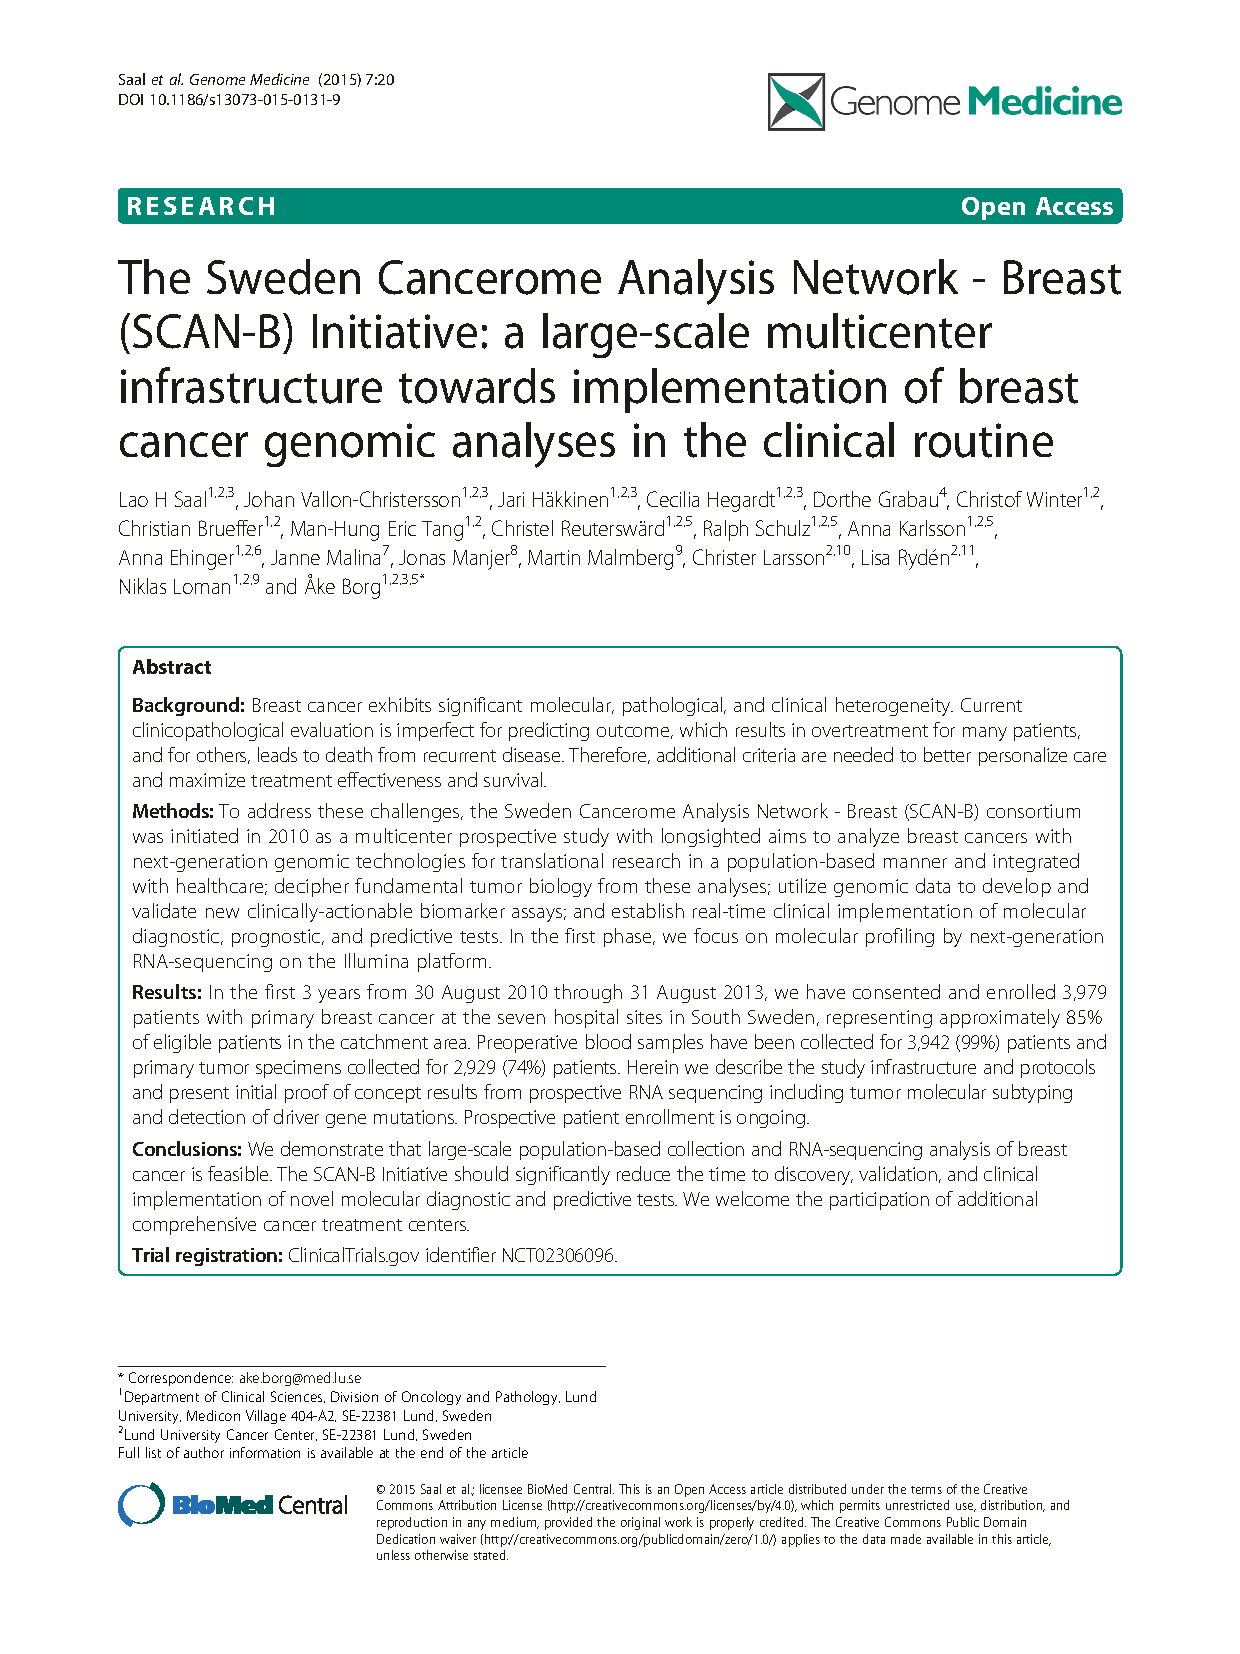
\includepdf[pages=-,width=1.00\textwidth,pagecommand={\thispagestyle{plain}}]{paper-1-SCANB-GenomeMed.pdf}
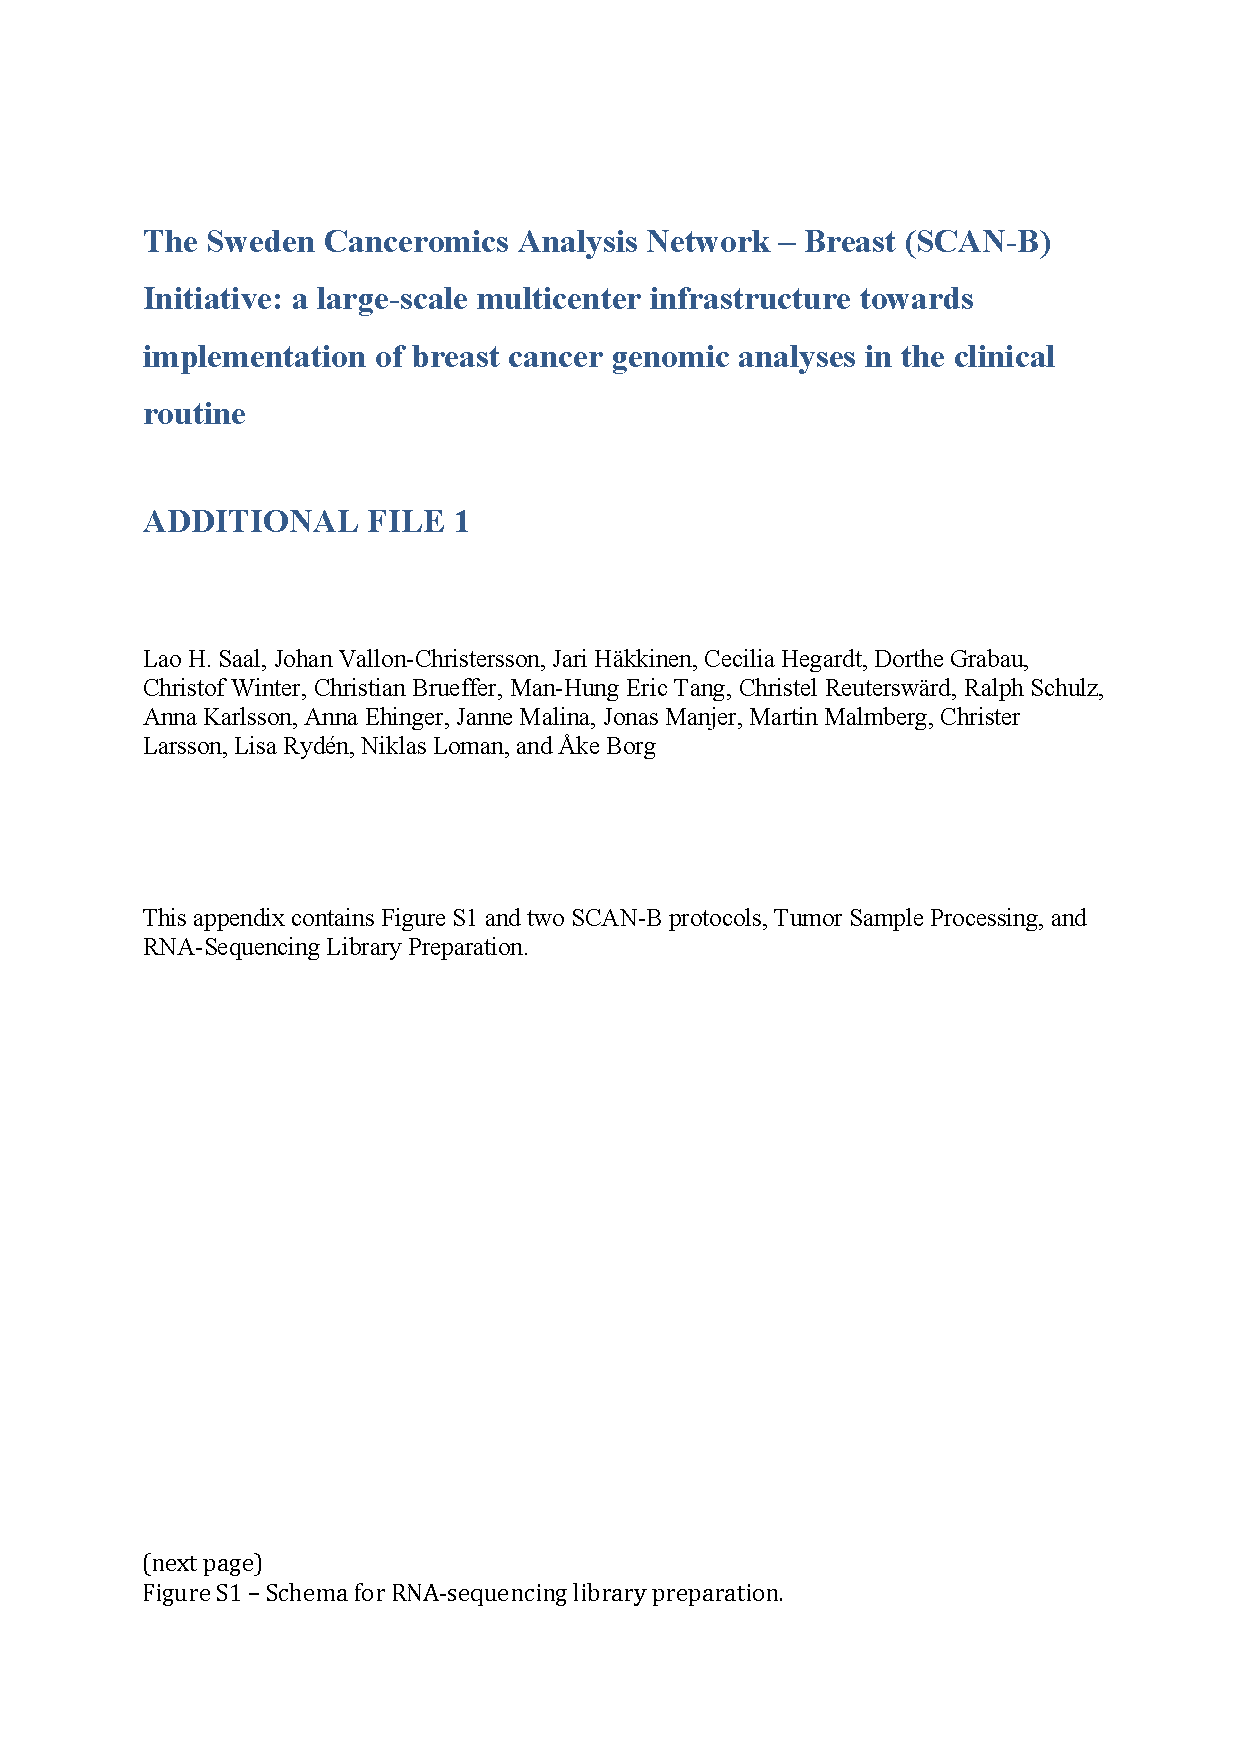
\includepdf[pages=-,width=1.00\textwidth,pagecommand={\thispagestyle{plain}}]{paper-1-supp-file1.pdf}
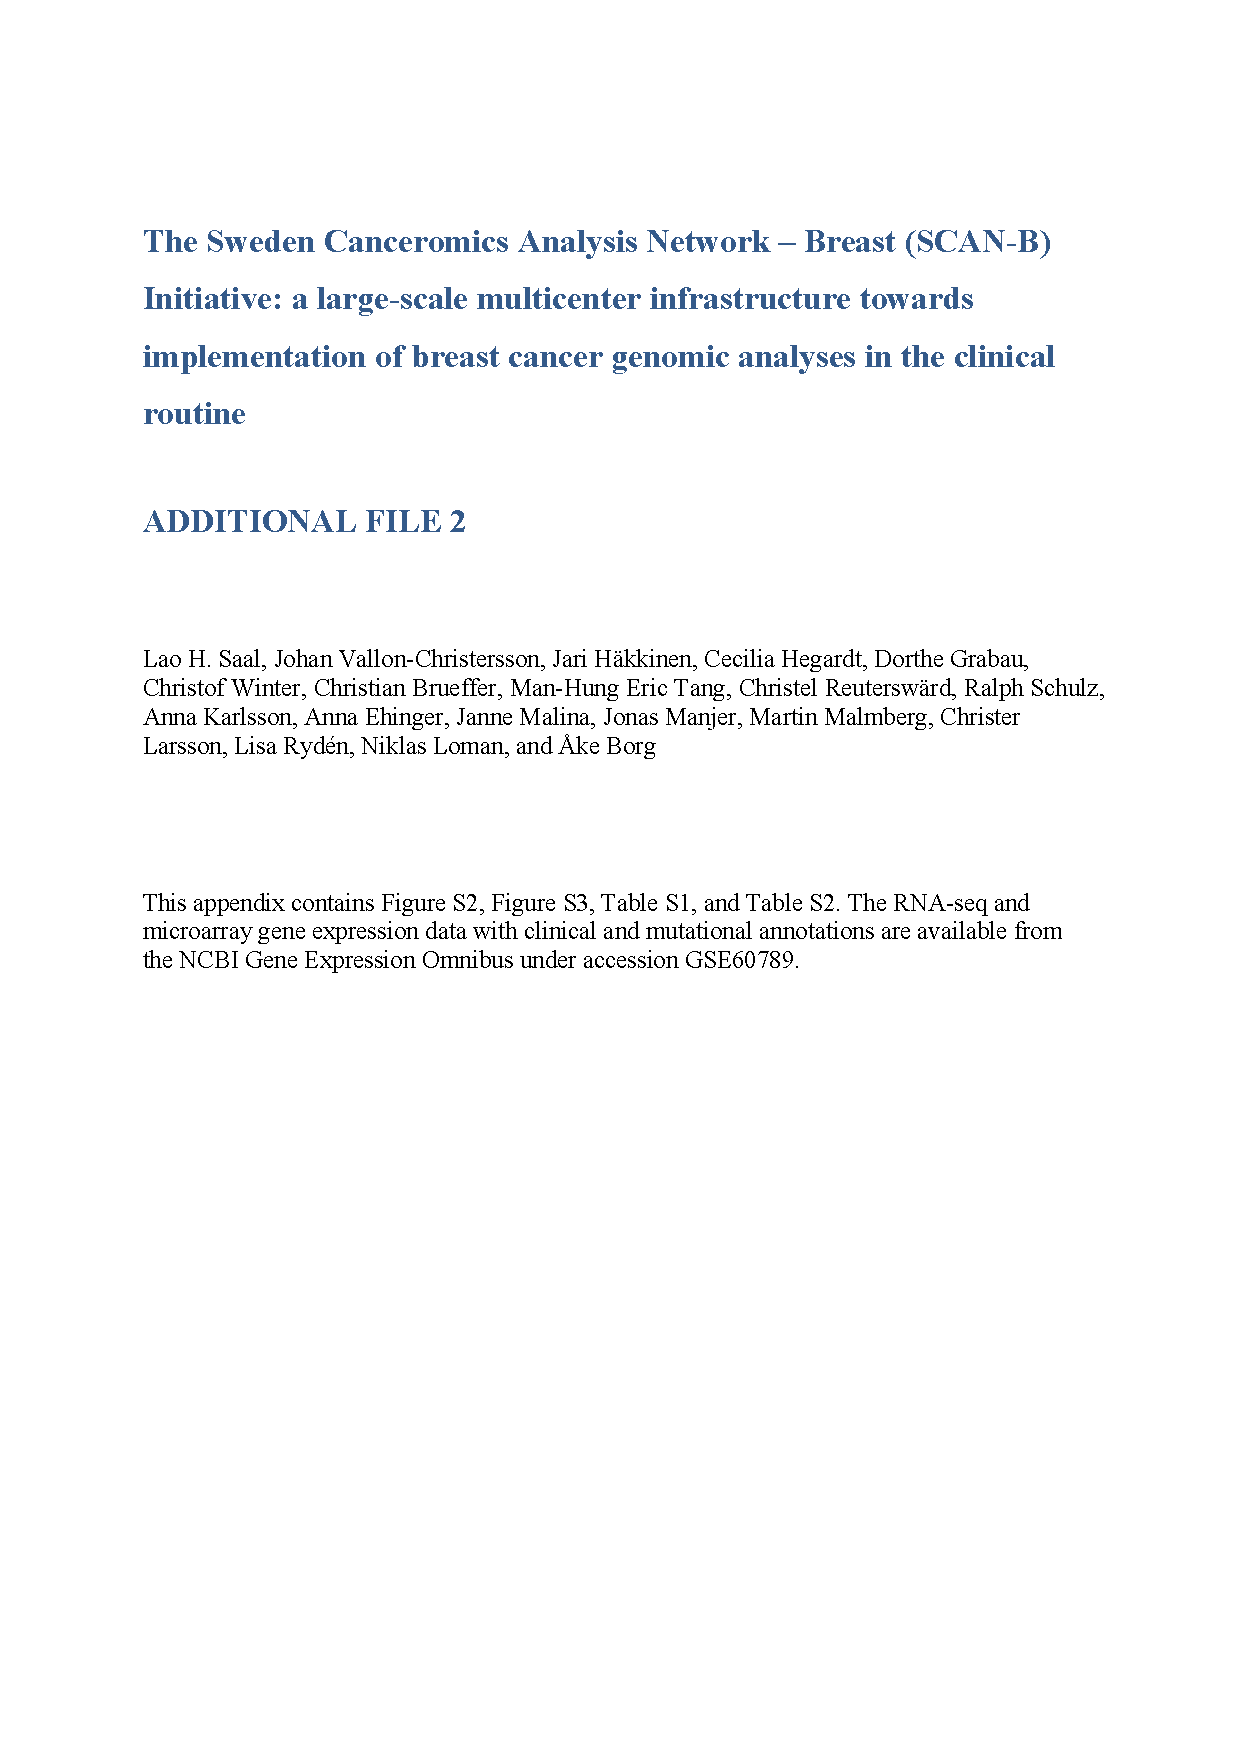
\includepdf[pages=-,width=1.00\textwidth,pagecommand={\thispagestyle{plain}}]{paper-1-supp-file2.pdf}
\restoregeometry


% ------------------
% PAPER II
% ------------------
\cleardoublepage
\addcontentsline{toc}{chapter}{Study \II: TopHat-Recondition: A post-processor for TopHat unmapped reads}
\thispagestyle{empty}

\newgeometry{right=\myPaperIndicatorLength}
\vspace*{5cm}  % IMPORTANT: Increase by 2cm each time.
\marginpar{\PaperBox[minimum width=\myPaperIndicatorLength]{{\color{white} \fontsize{20}{30}{\selectfont{\bf Study II}}}}} % Change the Roman number here
\restoregeometry

\vfill
\cleardoublepage
\newgeometry{left=0mm, right=0mm, top=0mm, bottom=0mm}
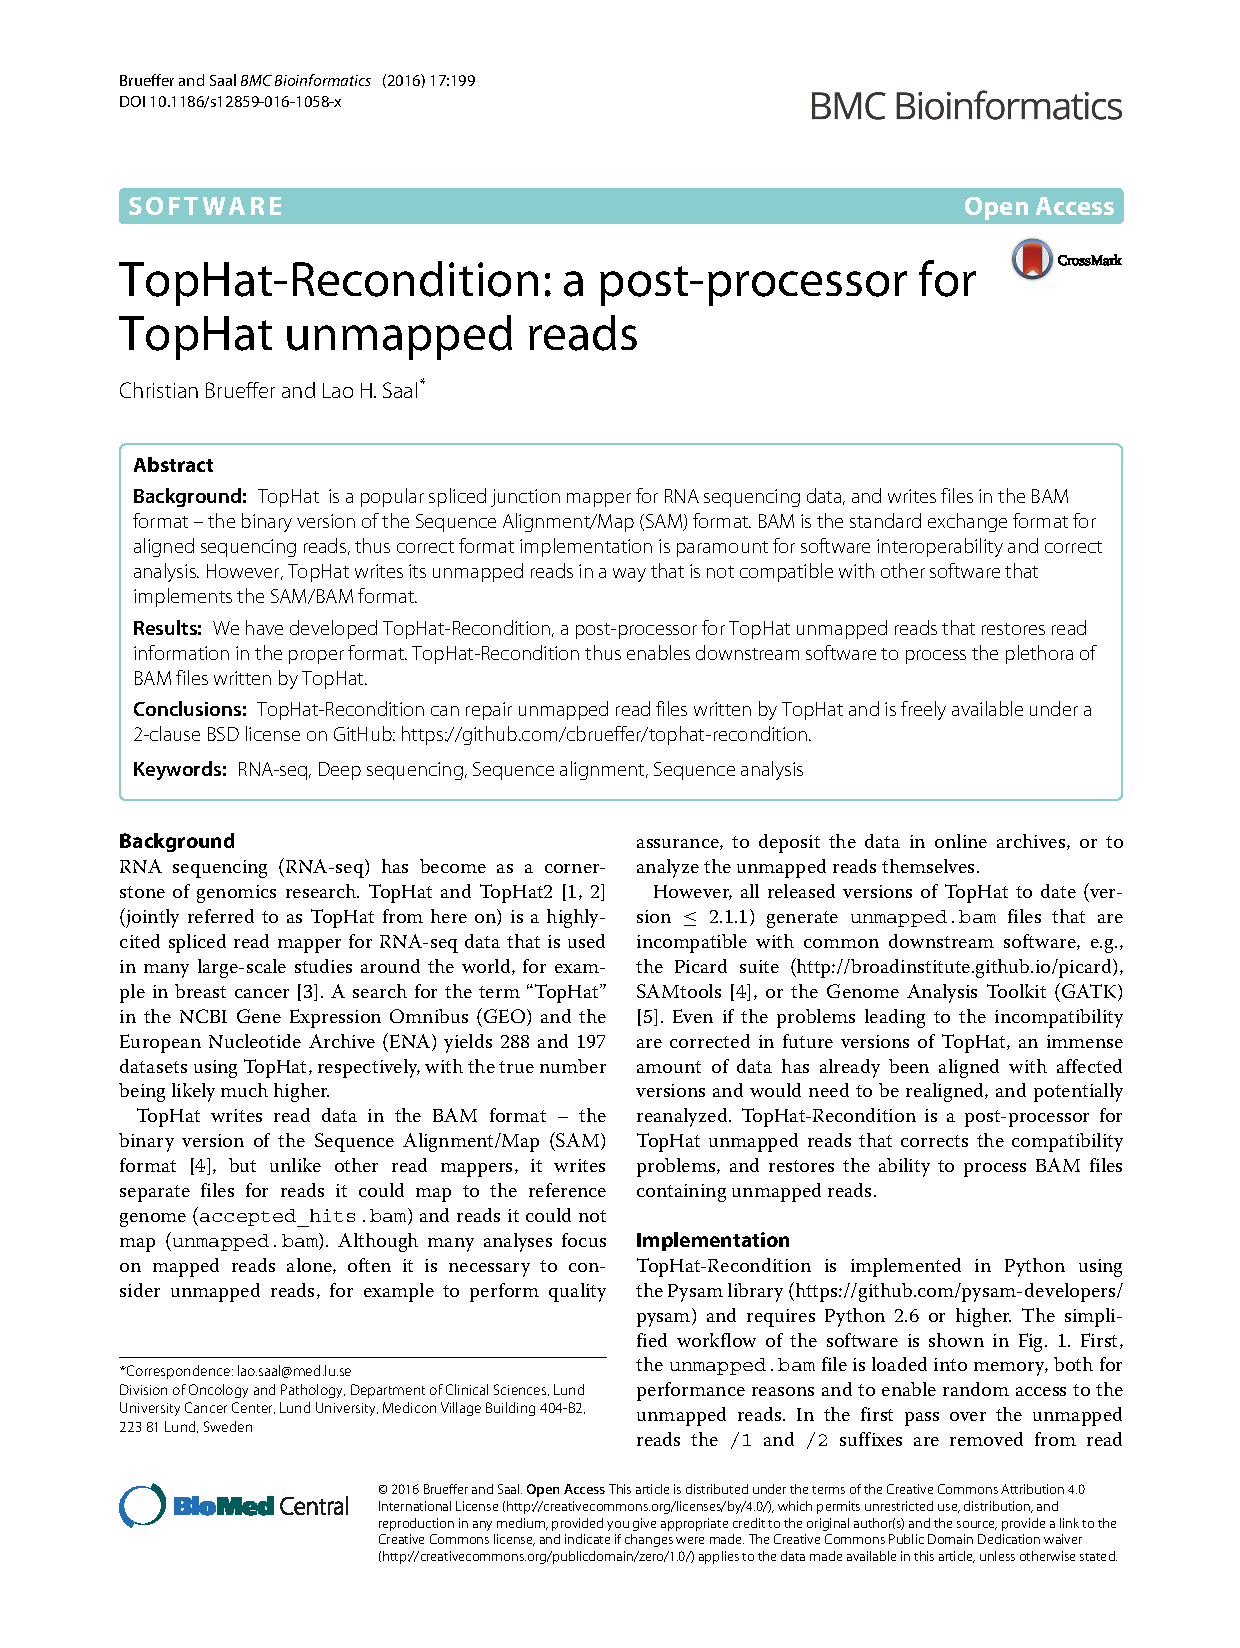
\includepdf[pages=-,width=1.00\textwidth,pagecommand={\thispagestyle{plain}}]{paper-2-TopHatRecondition-BMCBioinf.pdf}
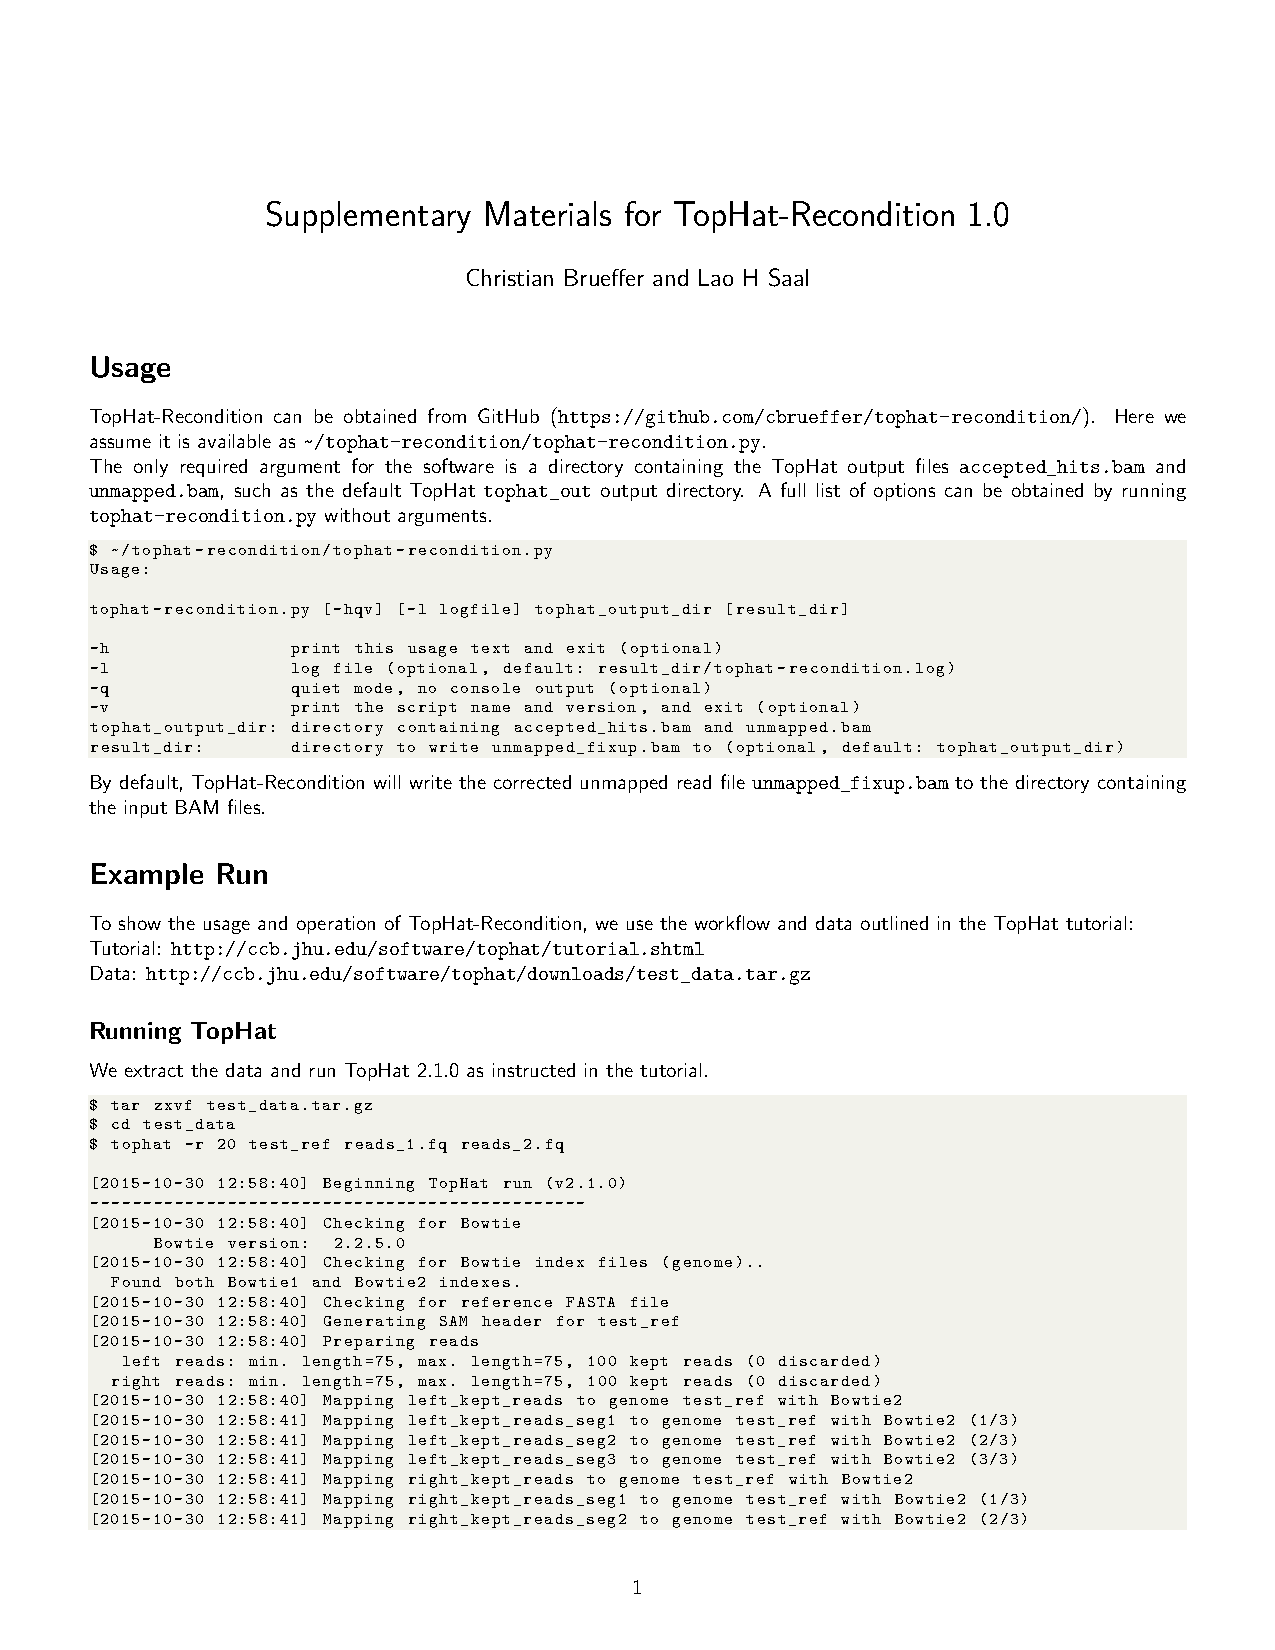
\includepdf[pages=-,width=1.00\textwidth,pagecommand={\thispagestyle{plain}}]{paper-2-supp-file.pdf}
\restoregeometry


% ------------------
% PAPER III
% ------------------
\cleardoublepage
\addcontentsline{toc}{chapter}{Study \III: Clinical Value of RNA Sequencing-Based Classifiers for Prediction of the Five Conventional Breast Cancer Biomarkers: A Report From the Population-Based Multicenter Sweden Cancerome Analysis Network--Breast Initiative}
\thispagestyle{empty}

\newgeometry{right=\myPaperIndicatorLength}
\vspace*{7cm}  % IMPORTANT: Increase by 2cm each time.
\marginpar{\PaperBox[minimum width=\myPaperIndicatorLength]{{\color{white} \fontsize{20}{30}{\selectfont{\bf Study III}}}}} % Change the Roman number here
\restoregeometry

\vfill
\cleardoublepage
\newgeometry{left=0mm, right=0mm, top=0mm, bottom=0mm}
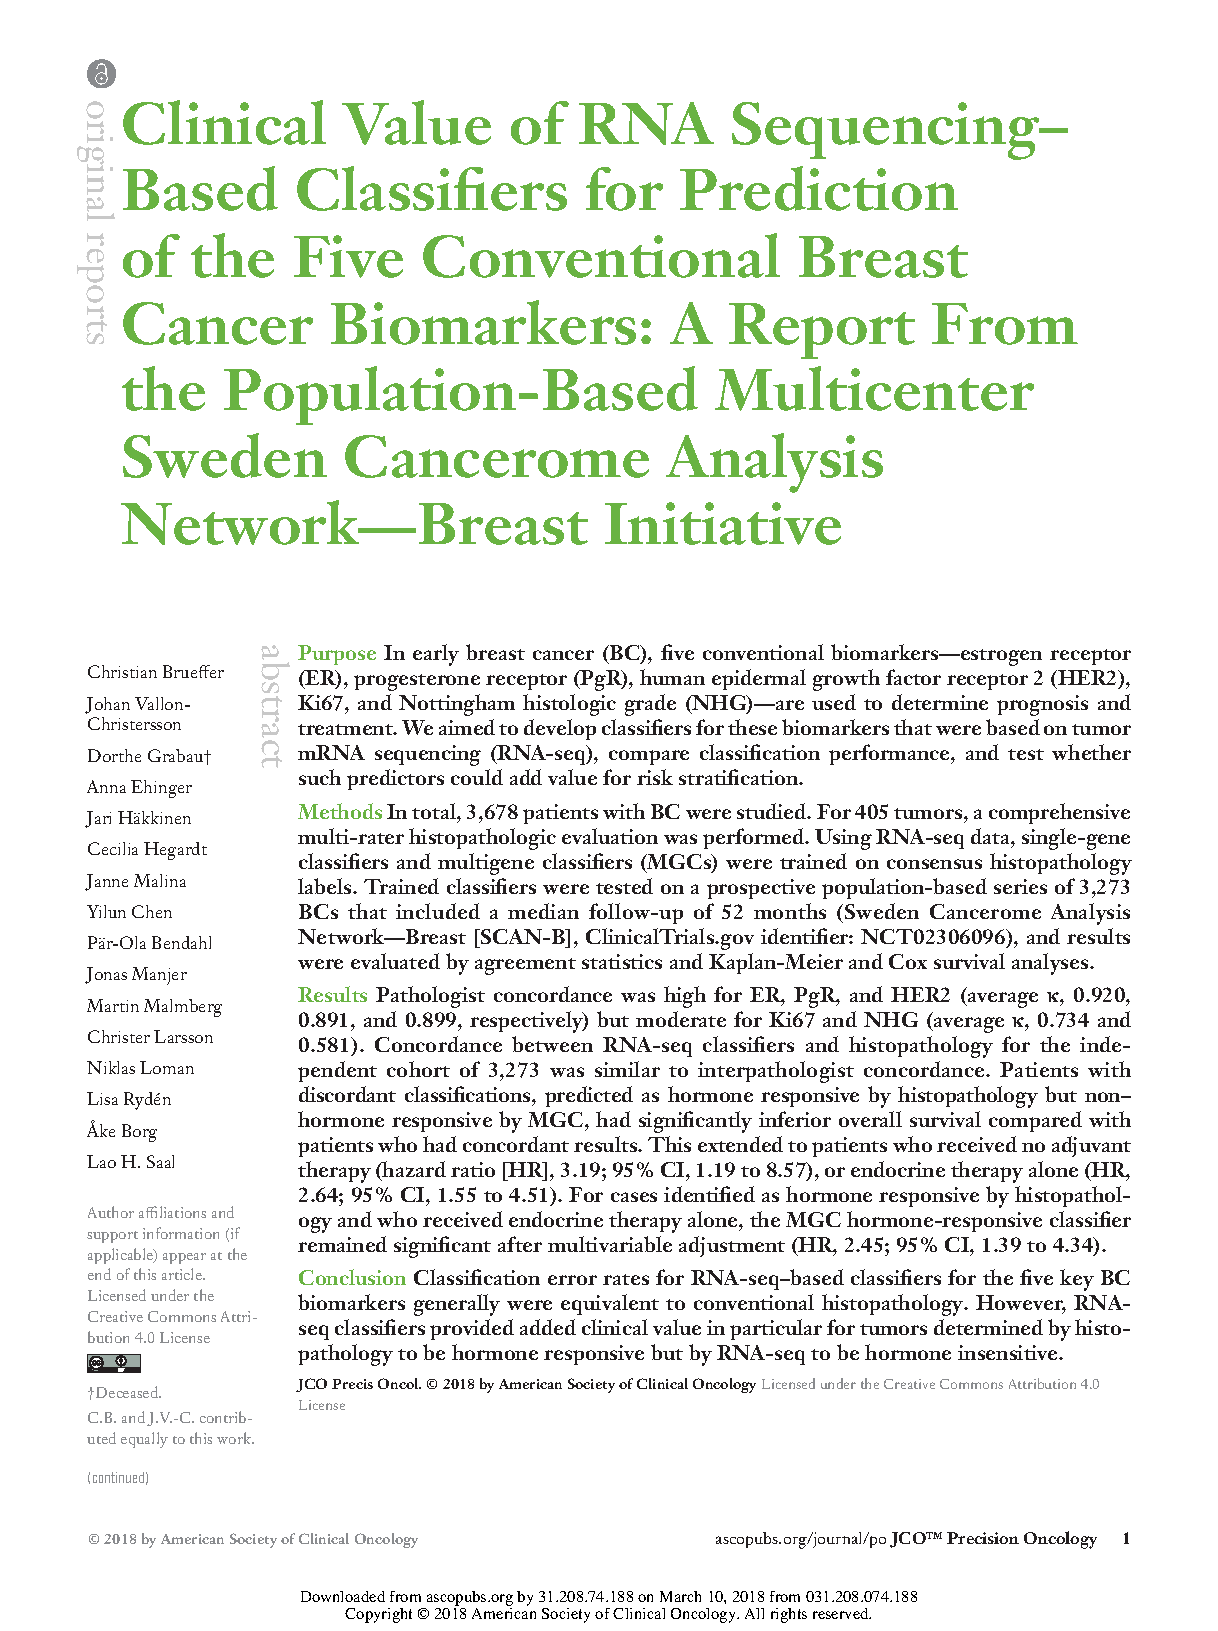
\includepdf[pages=-,width=1.00\textwidth,pagecommand={\thispagestyle{plain}}]{paper-3-BiomarkerPrediction-JCOPrecisOncol.pdf}
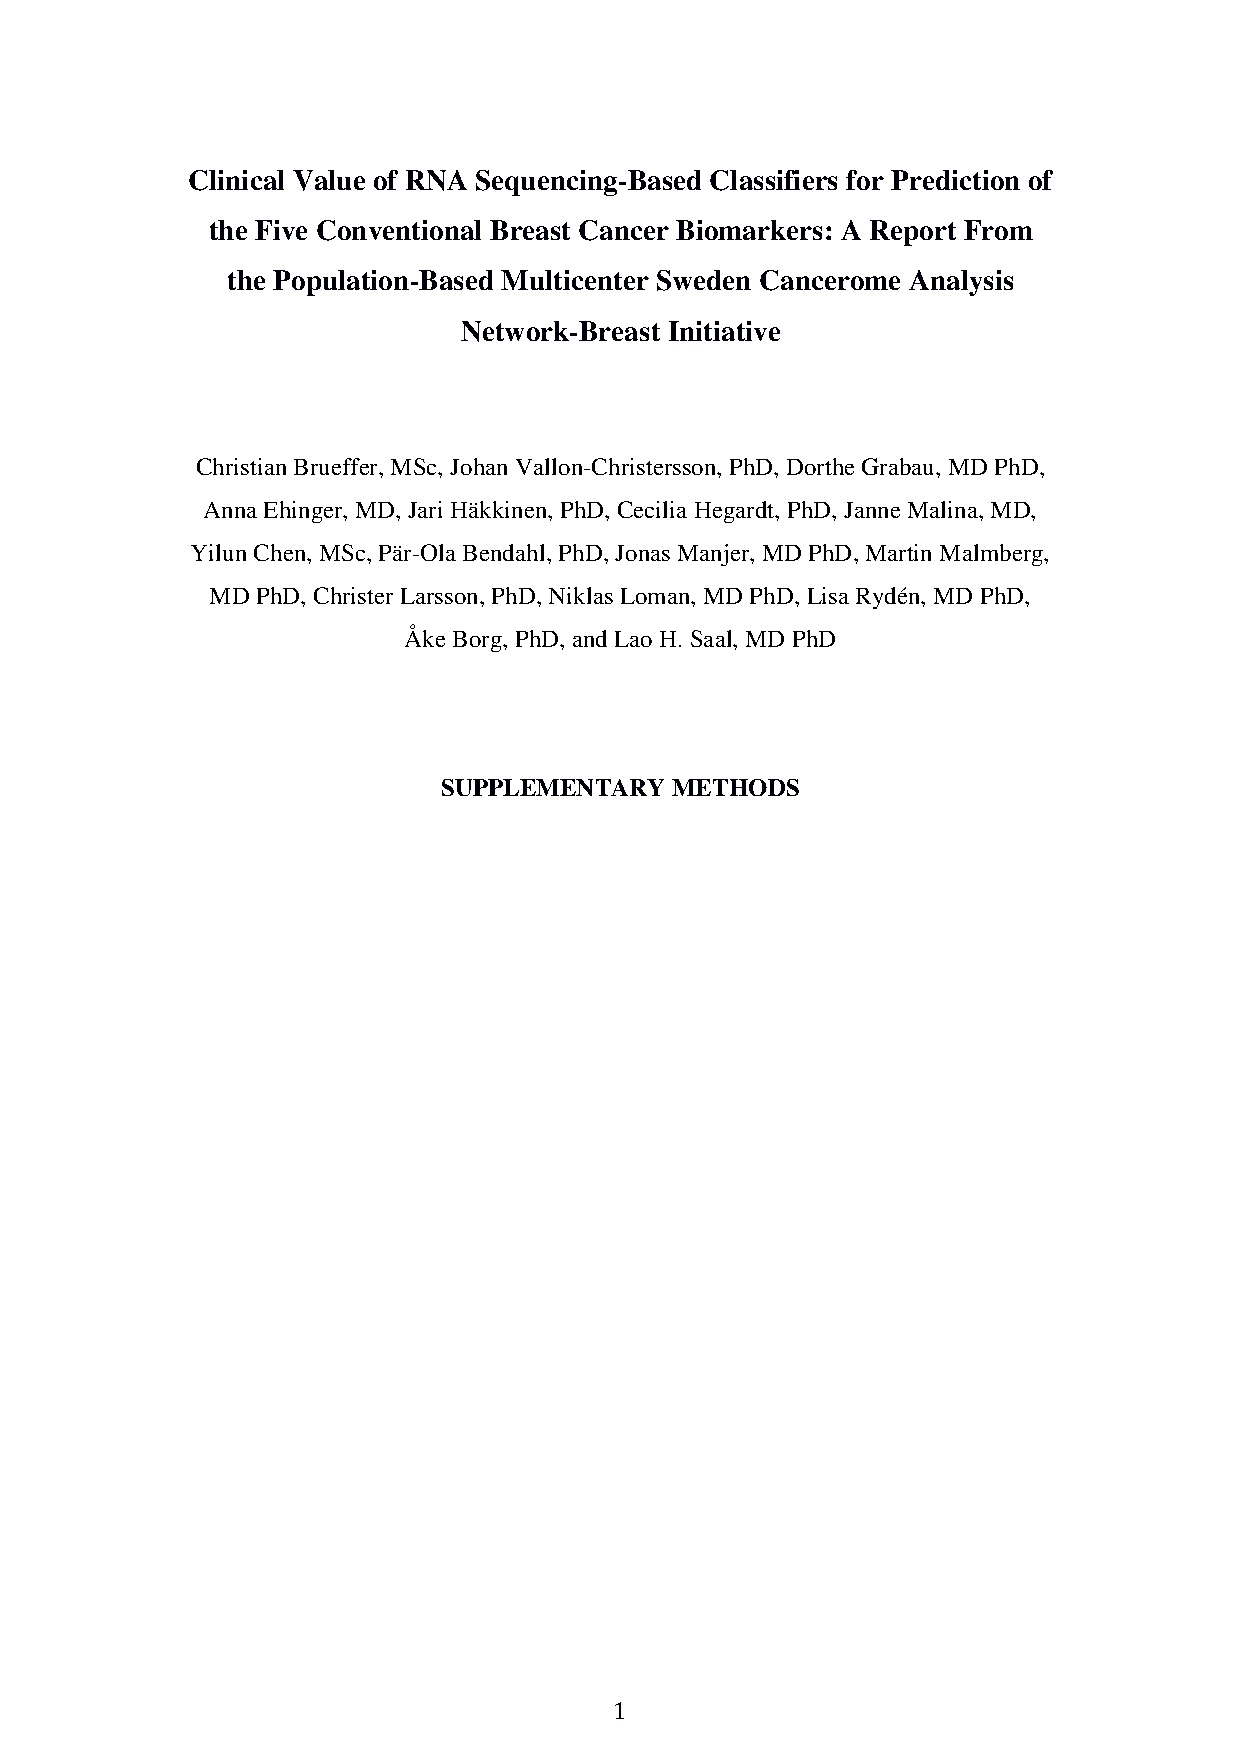
\includepdf[pages=-,width=1.00\textwidth,pagecommand={\thispagestyle{plain}}]{paper-3-supp-methods.pdf}
\restoregeometry


% ------------------
% PAPER IV
% ------------------
\cleardoublepage
\addcontentsline{toc}{chapter}{Study \IV: The mutational landscape of the SCAN-B real-world primary breast cancer transcriptome}
\thispagestyle{empty}

\newgeometry{right=\myPaperIndicatorLength}
\vspace*{9cm}  % IMPORTANT: Increase by 2cm each time.
\marginpar{\PaperBox[minimum width=\myPaperIndicatorLength]{{\color{white} \fontsize{20}{30}{\selectfont{\bf Study IV}}}}} % Change the Roman number here
\restoregeometry

\vfill
\cleardoublepage
\newgeometry{left=0mm, right=0mm, top=0mm, bottom=0mm}
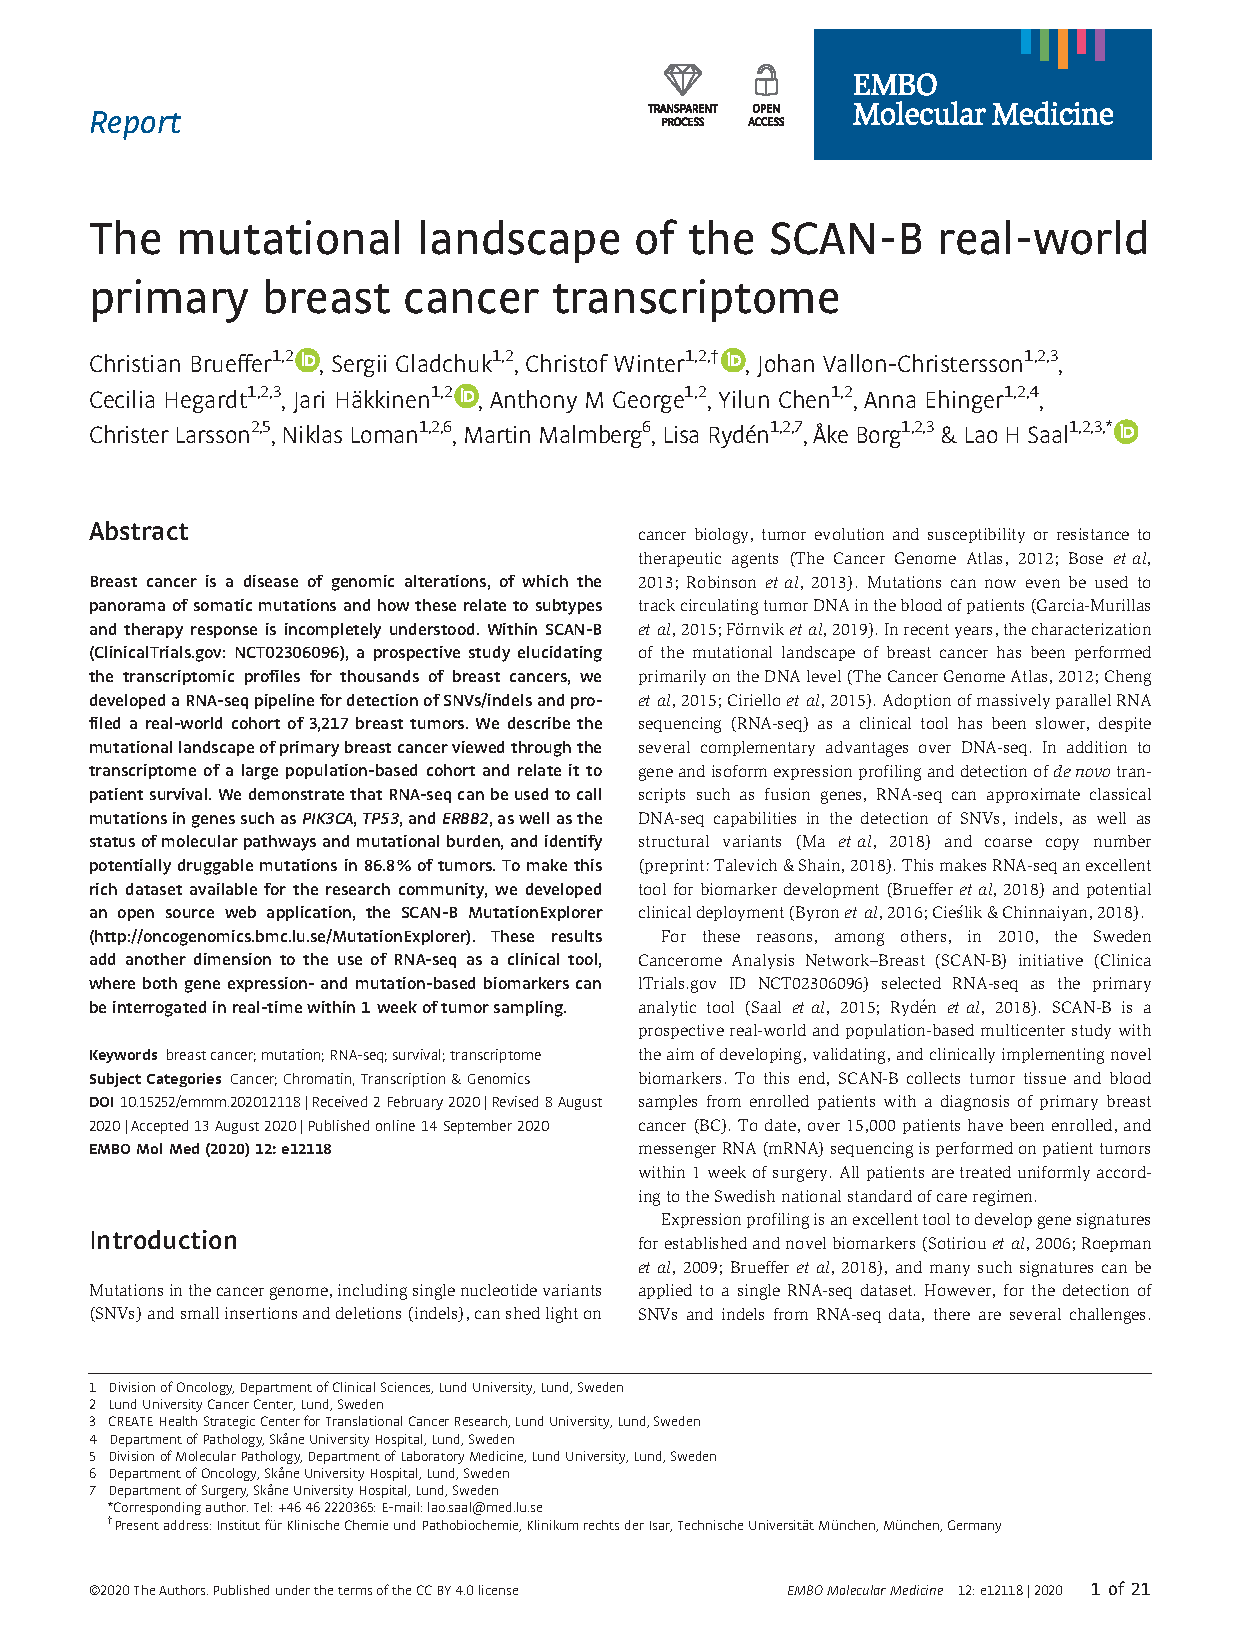
\includepdf[pages=-,width=1.00\textwidth,pagecommand={\thispagestyle{plain}}]{paper-4-MutationLandscape-EMBOMolMed.pdf}
\restoregeometry

\end{document}